\documentclass[thesis=M,english]{FITthesis}[2012/10/20]

% graphics files inclusion
\usepackage{graphicx}
% subfigures
\usepackage{subfig}
% advanced maths
\usepackage{amsmath}
\usepackage{amsthm}
\usepackage{amssymb}
% directory tree visualisation
\usepackage{dirtree}
% tikz package and the mindmap library
\usepackage{tikz}
\usetikzlibrary{arrows,mindmap,shapes.geometric}

\department{Department of Applied Mathematics}
\title{Neural Networks Based Domain Adaptation in Spectroscopic Sky Surveys}
\authorGN{Ondřej}
\authorFN{Podsztavek}
% author's name without academic degrees
\author{Ondřej Podsztavek}
\authorWithDegrees{Bc. Ondřej Podsztavek}
\supervisor{Petr Škoda}
% TODO acknowledgements
\acknowledgements{}
% TODO english abstract
\abstractEN{}
% TODO czech abstract
\abstractCS{}
\placeForDeclarationOfAuthenticity{Prague}
\keywordsEN{
	domain adaptation,
	neural networks,
	deep learning,
	astronomy
}
\keywordsCS{
	doménová adaptace,
	neuronové sítě,
	hluboké učení,
	astronomie
}
% select according to the desired license (integer 1-6)
\declarationOfAuthenticityOption{2}
% TODO optional thesis URL
%\website{}

\theoremstyle{definition}
\newtheorem{definition}{Definition}

% TODO delete
%\includeonly{domain_adaptation}

\begin{document}

\chapter{Introduction}

How to use neural network based domain adaptation to extract knowledge from the source domain of astronomical spectral data
and apply it to the target astronomical spectral data?

In this work, we would like to prove that astronomical spectroscopy can benefit from domain adapatation (DA).
Previous research has shown that DA can overcome the problem of analysis data from different distribution in one experiment.
In the first chapter~\ref{da_chapter}, we provide a summary of theory of DA, neural networks in DA and DA in astronomy.
Then, in chapter~\ref{data_chapter}, we describe current spectroscopic sky surveys
which might be source of suitable astronomical spectral data.
In experiments~\ref{exp_chapter}, we try to show the benefits of neural DA in astronomy.
Consider that our work is limited to astronomical spectroscopy and neural models.
Having said that, we will apply these methods\dots{}

\section{Problem Definition and Motivation}

The goal of this thesis is the analysis of the impact of domain adaptation in astronomical archives with a focus on neural networks
that would allow using labelled data from one ground-based telescope or space mission archive to discover knowledge in another archive.
Current astronomy has been the primary customer of scalable Big data handling and analysis requirements due to its petabyte-scale archives,
where an advanced machine learning is an indispensable part of workflows leading to new discoveries.

\chapter{Spectroscopic Sky Surveys}
\label{data_chapter}

% TODO chapter introduction

Select suitable dataset of astronomical spectra for experiments.

To understand this work we need first to introduce the spectral
data because we are interested in classifying them.

\section{Astronomical Spectroscopy}

Almost all we know about the universe outside our solar system
is based on the analysis of ligth, i.e. \textit{electromagnetic} (EM) radiation
by observing its flux, time variations, etc.~\cite{appenzeller2012}
Spectroscopy started when Issac Newton carried out the experiment of light decomposition throgh a prism in 1666.
Next, Thomas Young has shown that light behaves like a wave.
However, EM radiation exhibits also particle nature.

The particles of EM radiation are photons.
Photons has no mass but transport energy and have momentum.
Every photon has an associated frequency \(\nu\)
of the corresponding EM wave giving it a energy
by the Planck--Einstein relation:

\begin{equation}
	E = h \nu,
	\label{planck_einstein_equation}
\end{equation}

where \(h\) is the Planck constant and \(\nu\) is frequency of the photon.
Therefore, higher frequency means higher energy.
All photons in vacuum move in the speed of light \(c\).
The frequency \(\nu\) is related to the wavelength \(\lambda\):

\begin{equation}
	\nu = \frac{c}{\lambda},
	\label{frequency_wavelength_equation}
\end{equation}

where \(c\) is the speed of light.
Combining equations~\ref{planck_einstein_equation} and \ref{frequency_wavelength_equation} gives:

\begin{equation}
	E = h \frac{c}{\lambda}.
	\label{energy_wavelength}
\end{equation}

We see that energy of a photon is inversly proportional to wavelength \(\lambda\).~\cite{trypsteen2017}

Secondly, EM radiation has the wave nature. 
EM wave also propagetes in the speed of light \(c\) and transfers energy.
Again the higher the frequency the more energy it carries.~\cite{cochard2018}

EM wave can be decomposed (by a prism or a diffraction grating)
as a function of its wavelength \(\lambda\).
The complete decomposed spectrum of EM radiation is called the EM spectrum.
The visible light is only a tiny part of the complete spectrum of electromagnetic radiation.
The complete spectrum consists of \(\gamma\)~rays, X-rays, ultraviolet, visible light, infrared radiation, microwaves, radio waves (see Table~\ref{em_spectrum}).

\begin{table}
\begin{center}
\begin{tabular}{|l|r|}
	\hline
	Radiation type & Wavelength (m) \\ \hline \hline
	\(\gamma\) ray & \(10^{-12}\) \\ \hline
	X-ray & \(10^{-10}\) \\ \hline
	Ultraviolet & \(10^{-8}\) \\ \hline
	Visible & \(0.5 \times 10^{-6}\) \\ \hline
	Infrared & \(10^{-5}\) \\ \hline
	Microwave & \(10^{-2}\) \\ \hline
	Radio & \(10^{3}\) \\ \hline
\end{tabular}
\end{center}
\caption{Parts of electromagnetic spectrum}
\label{em_spectrum}
\end{table}

EM radiation is produced by either heating up matter or by exciting atoms.
The blackbody is a physical model of spectral radiation \(B(\lambda, T)\).
Max Planck derived the spectral distributon of a black body.
Heating transforms into an emission of EM radiation at all wavelengths
with an energy distribution as a function of wavelength
which only depends on the temperature and is described by Planck's law:

\begin{equation}
	B(\lambda, T) = \frac{2 h c^2}{\lambda^5}
	\frac{1}{e^{\frac{hc}{\lambda k_{\mathrm{B}}T}} - 1}
\end{equation}

where \(k_{\mathrm{B}}\) is the Boltzmann constant 
and \(h\) is the Planck constant.
This phenomenon does not depend on the composition of the body
but only on its temperature.
The Wien's displacement law gives the wavelength of maximum intensity \(\lambda_{\max}\):

\begin{equation}
	\lambda_{\max} = \frac{b}{T}
\end{equation}

where \(b\) is the Wien's displacement constant.
Accordingly, we can derive the temperature \(T\) of an object
with known wavelength of maximum intesity \(\lambda_{\max}\):

\begin{equation}
	T = \frac{b}{\lambda_{\max}}.
\end{equation}

where \(b\) is the Wien's displacement constant.~\cite{cochard2018}

We consider stars to be black bodies
because they are objects hotter than its environmenti
and emit electromagnetic radiation.
Therefore, all EM radiation of a star is determined only by its temperature.
The other way around, with the Wien's displacement law
we can estimate the absolute temperature \(T\) of a star.~\cite{trypsteen2017}

The undisturbed profile of a continuum level \(I(\lambda)\)
represents roughly the temperature dependence on
blackbody radiation characteristics \(B(\lambda, T)\).

% TODO show image continuum

Secondly, EM radiation can be emitted by exciting atoms.
Therefore, EM radiation carries information about stars and planets
made of matter across the universe.
The energy carried by EM radiation interacts with matter in following ways:

\begin{itemize}
	\item \textit{emission} occurs when EM radiation propages throught a gas
		because the atoms of the gas might exite ane emit EM radiation;
	\item \textit{absorption} happens when a gas absorbs some wavelengths
		of the EM radiation.
\end{itemize}

Fraunhofer was also one of the first to observe dark lines in the solar spectrum
and David Brewster postulated that the dark lines correspond to absoption from gas in the way of light travelling towards us.
Robert Wilhelm Bunsen and Gustav Kichhoff showed that each chemical element has its own set of spectral lines
and Kichhoff established the three famous laws describing the three types of spectra:

\begin{itemize}
	\item the spectrum of a conventional light bulb is a continuous rainbow (called \textit{continuos spectrum});
	\item if a cloud of gas lies between a detector and a bulb,
		the cloud can absorb specific wavelength making what an \textit{absorption-line spectrum};
	\item if a cloud emits light itself its spectrum is called an \textit{emission-line spectrum}.
\end{itemize}

Real astronomical spectra are usually a combination of these types.
Therefore, spectrocopy can be used for chemical analysis of matter.
Then, at the beginning of the twentieth century,
the invention quantum mechanics help us to understand the origin of spectral lines.

We model matter as made of atoms.
An atom has a specific number of electrons
which are place in particular orbits of the atom.
Electrons in an orbit have a specic energy level.
We know from quantum mechanics that an electron can change energy level by an exchange of energy in form of a photon.
The energy transfer is not continuous.
The energy has to precisily correspond to the difference in the energy levels.
Therefore the change produces a EM radation with an energy \(E\) in the wavelength \(\lambda\)
according to Planck--Einstein relation~\ref{energy_wavelength}.
Therefore, the specific set of energy levels of a atom detemines
if photons are either absorped or emitted by it.
This is a direct consequence for spectroscopy.~\cite{cochard2018}

The fact that each atom,
ion or molecule possesses a unique set of energy levels
causes emission and absorption lines at specific wavelengths in spectra.
Spectral lines correspond to the wavelengths of light absorbed by chemicals on the surface of the star.
Therefore, positions of emission and absorption lines can tell us objects composition.
We display spectra as bands of light that is a projection of light
that passes through a prism on a wall (see Fig.~\ref{solar_spectrum})
called \textit{two-dimensional} spectra.~\cite{cochard2018}

\begin{figure}
% source https://solarsystem.nasa.gov/resources/390/the-solar-spectrum/
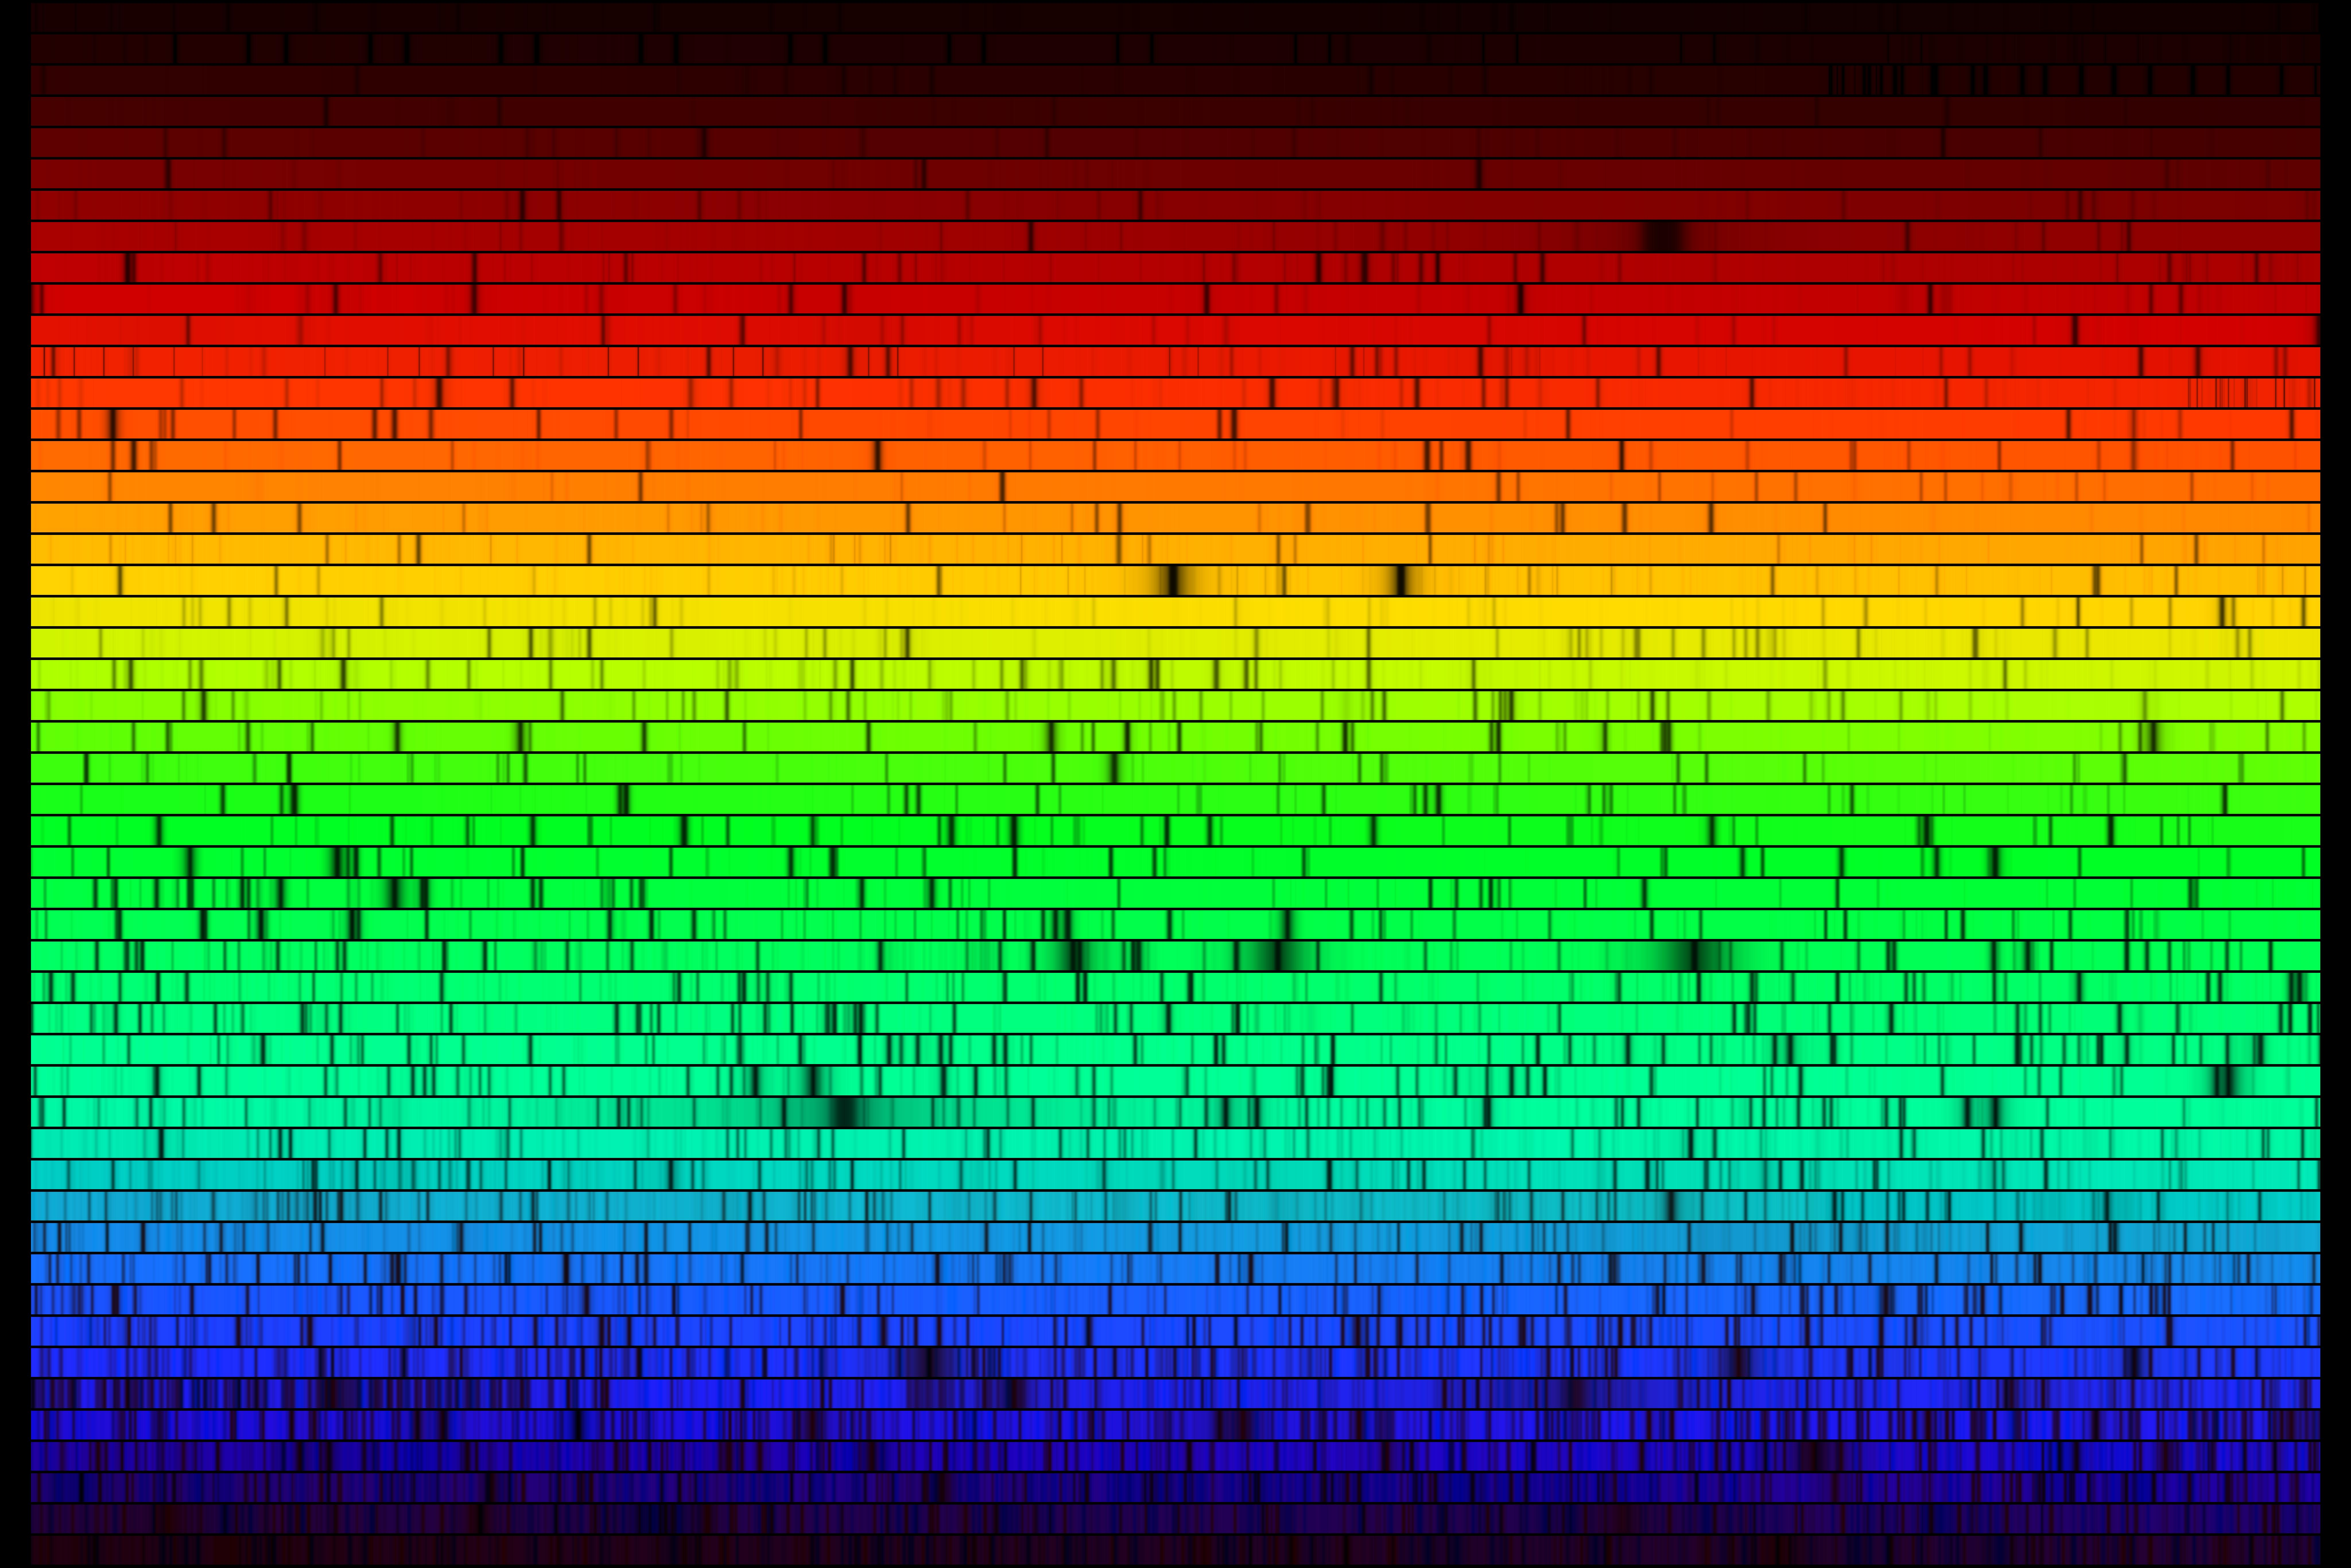
\includegraphics[width=\textwidth]{img/solarspectrum.jpg}
\caption[The Solar spectrum]{
	The specturm of the Sun. (Image by \href{https://solarsystem.nasa.gov/resources/390/the-solar-spectrum/}{NASA}.)
}
\label{solar_spectrum}
\end{figure}

A more reasonable way is to display spectra as graphs of intensities of the light as the vertical axis and wavelengths as the horizontal axis:
called a \textit{one-dimensional spectral profile}.~\cite{cochard2018}
This representation of a astronomical spectrum can be seen as a one-dimensional image.~\cite{bennett2005}

% TODO one-dimensional spectrum

% TODO Christian Doppler discoverd the Doppler effect that allowed to measure the motion of celestial objects using Doppler shift in its spectrum.

Joseph von Fraunhofer was the first to observe spectra of stars by using spectroscope in combination with telescope.
Nowadays, new technologies have advanced spectroscopic observations
(CCD detectors, optical fibers and computing power).~\cite{cochard2018}
Telescopes are giant eyes that can collect much more light that an eye of a human.
A telescope is composed of mirror that lead light into a spectrograph.
A spectrograph contains a diffraction grating and a \textit{charge-coupled device} (CCD) camera.
Diffration grating was invented by Fraunhofer based on the wave nature of light.
Diffration grating can disperse the light collected by a telescope into a spectra
while allowing greater dispersion than prisms.
on gratings are one of the essential parts of modern spectroscopes
Then the dispersed specturm reveals objects composition, speed, temperature
and more.~\cite{bennett2005}

Photons carry information about observed objects
to a pixel of a CCD camera in a telescope.
CCD cameras require the particle nature of light (electromagnetic radiation).~\cite{trypsteen2017}

The most important parameters of a telescope are
\textit{resolving power}, \textit{signal-to-noise ration}
and \textit{signal-to-noise ration}.

Resolving power \(R\) experess capacity of a telescope to oberve details of a spectrum.
Resolving power is defined as:

\begin{equation}
	R = \frac{\lambda}{\Delta \lambda}
\end{equation}

where \(\lambda\) is considered wavelength
and \(\Delta \lambda\) is the smallest visible detail.

% TODO is it a parameter of a telescope or spectrum?
\textit{Signal-to-noise ratio} (SNR) is a parameter of our instrument.
We can trust our measurment when signal is high in compared to nise.~\cite{cochard2018}

\textit{Full width at half maximum} (FWHM) is the measurement of the width of a spectral line
at the half of its maximum intensity measured from the continuum.
FWHM is determined by the width of a slit which makes the broadening of a line.
A perfect instrument would have an infinitely thin line.

\section{Quasi-Stellar Objects}

Quasi-stellar (star-like) objects (also known as \textit{quasars} and abbreviated \textit{QSO}) are the most luminious \textit{active galactic nuclei} (AGNs).~\cite{beckmann2013}

The physical model is a supermassive black hole surrounded by a gaseous accretion disk.
A QSO generates energy by stress and friction in the disk outside ot the black hole because no light can escape the \textit{event horizont}.
The energy is in form of electromagnetic radiation and is the strongest in the ultraviolet band.
Moreover, QSOs exhibit big cosmological redshift.

QSOs were common in the early universe probably because galaxies have run out of matter: they stop to be so lumionious.
Therefore, QSOs help us to study the early universe.

There are different types of QSOs: radio-loud, radio-quiet, broad absorption-line, type II, red, optically violent variable, weak emission-line.

\begin{itemize}
	\item Physical definition of QSOs.
	\item Definition of QSOs according SDSS DR14Q.
	\item Why QSOs are suitable for experimenting with DA?
		QSOs have big redshift and CNNs are shift invariant.
		Searching for QSOs in different archives.
\end{itemize}

\begin{figure}
\begin{center}
\subfloat[Best image of bright quasar 3C 273][
	Best image of the bright quasar 3C 273
	(Image by \href{https://www.spacetelescope.org/images/potw1346a/}{ESA/Hubble} is licensed under CC BY 4.0)
	]{
	% TODO give credit https://www.spacetelescope.org/images/potw1346a/
	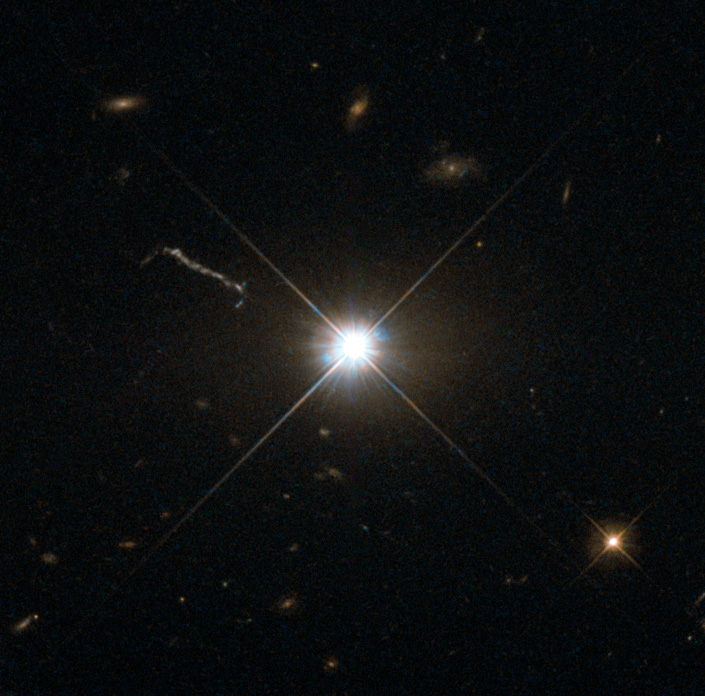
\includegraphics[height=0.45\textwidth]{img/potw1346a.jpg}
	}
\subfloat[Jet]{
	% TODO give credit https://chandra.harvard.edu/photo/2000/0131/index.html
	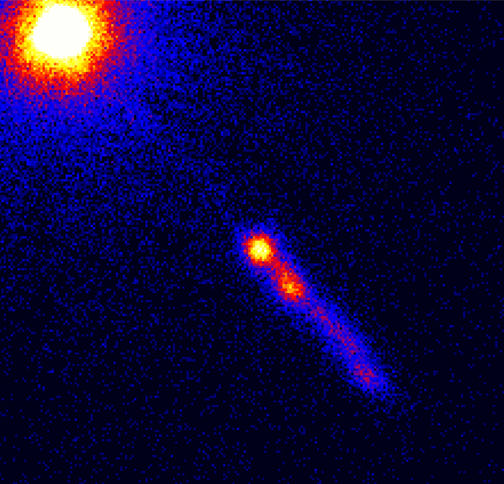
\includegraphics[height=0.45\textwidth]{img/0131_xray.jpg}
	}
\end{center}
\caption{
The first ever discover quasar 3C 273.
}
\label{3c_273}
\end{figure}

\begin{figure}
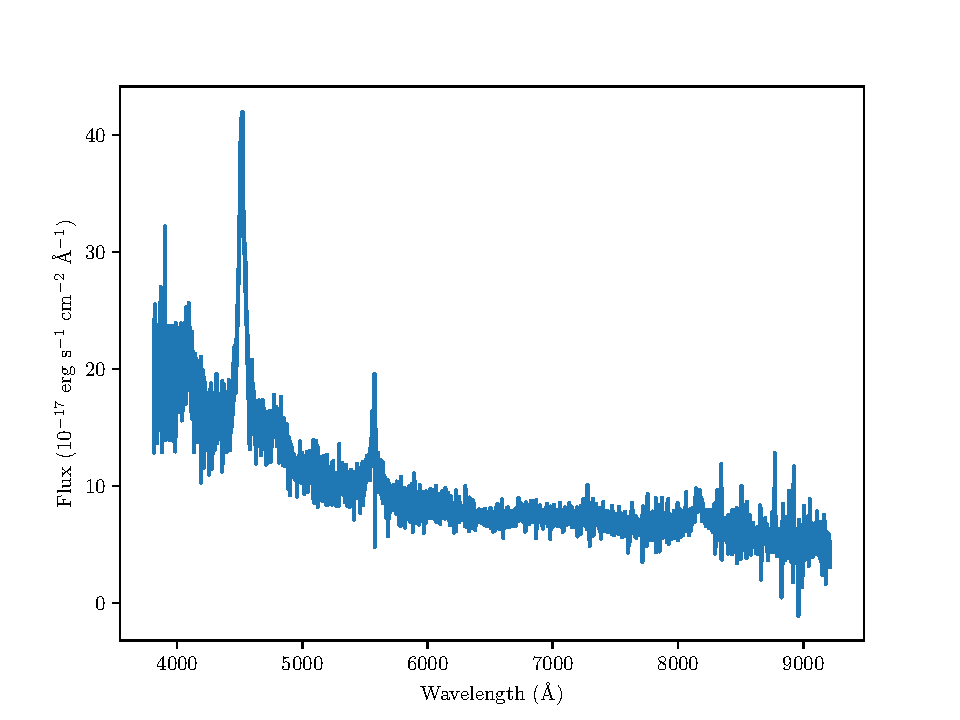
\includegraphics[width=\textwidth]{img/spec_3c_273.pdf}
\caption{Spectrum of the QSO 3C 273}
\label{3c_273_spectrum}
\end{figure}

\section{Large Spectroscopic Surveys}
\label{large_spec_surveys}

Since the discovery of first QSO,
there has been a huge progress in spectroscopy allowing observing
vast amount of spectra and QSOs.
It started with Bright Quasar Survey, Large Bright Quasar Survey (LBQS)
and 2dF Quasar Redshift Survey.
Their big successors are the \textit{Sloan Digital Sky Survey} (SDSS)
and the \textit{Large Sky Area Multi-Object Fiber Spectroscopic Telescope} (LAMOST)
that already contain millions of spectra.
We choose LAMOST and SDSS surveys for our experiments
because they offer large volume of data suitable for machine learning
and training neural networks for domain adaptation.

In the two following subsections,
we introduce the paramaters of their instruments,
their recent data releases and corresponding catalogs of QSOs.

\subsection{Sloan Digital Sky Survey}
\label{sdss}

SDSS is in opeation since 2000
and its telescope is designed to provide both a photometrically
and astrometrically calibrated imaging survey
and a spectroscopic survey of galaxies and QSOs.~\cite{york2000}

The SDSS survey uses a 2.5~m telescope located at the Apache Point Observatory, New Mexico (see~Figure~\ref{sdss_telescope}).
The telescope has 3\(^{\circ}\) fild of view due to the mirror.
The original spectrograph of the telescope was able to obtain 640 spectra
with a wavelength coverage 380--920~nm simultaneously
with spectral resolution \(R \sim 1\,800\).~\cite{gunn1998, york2000}

\begin{figure}
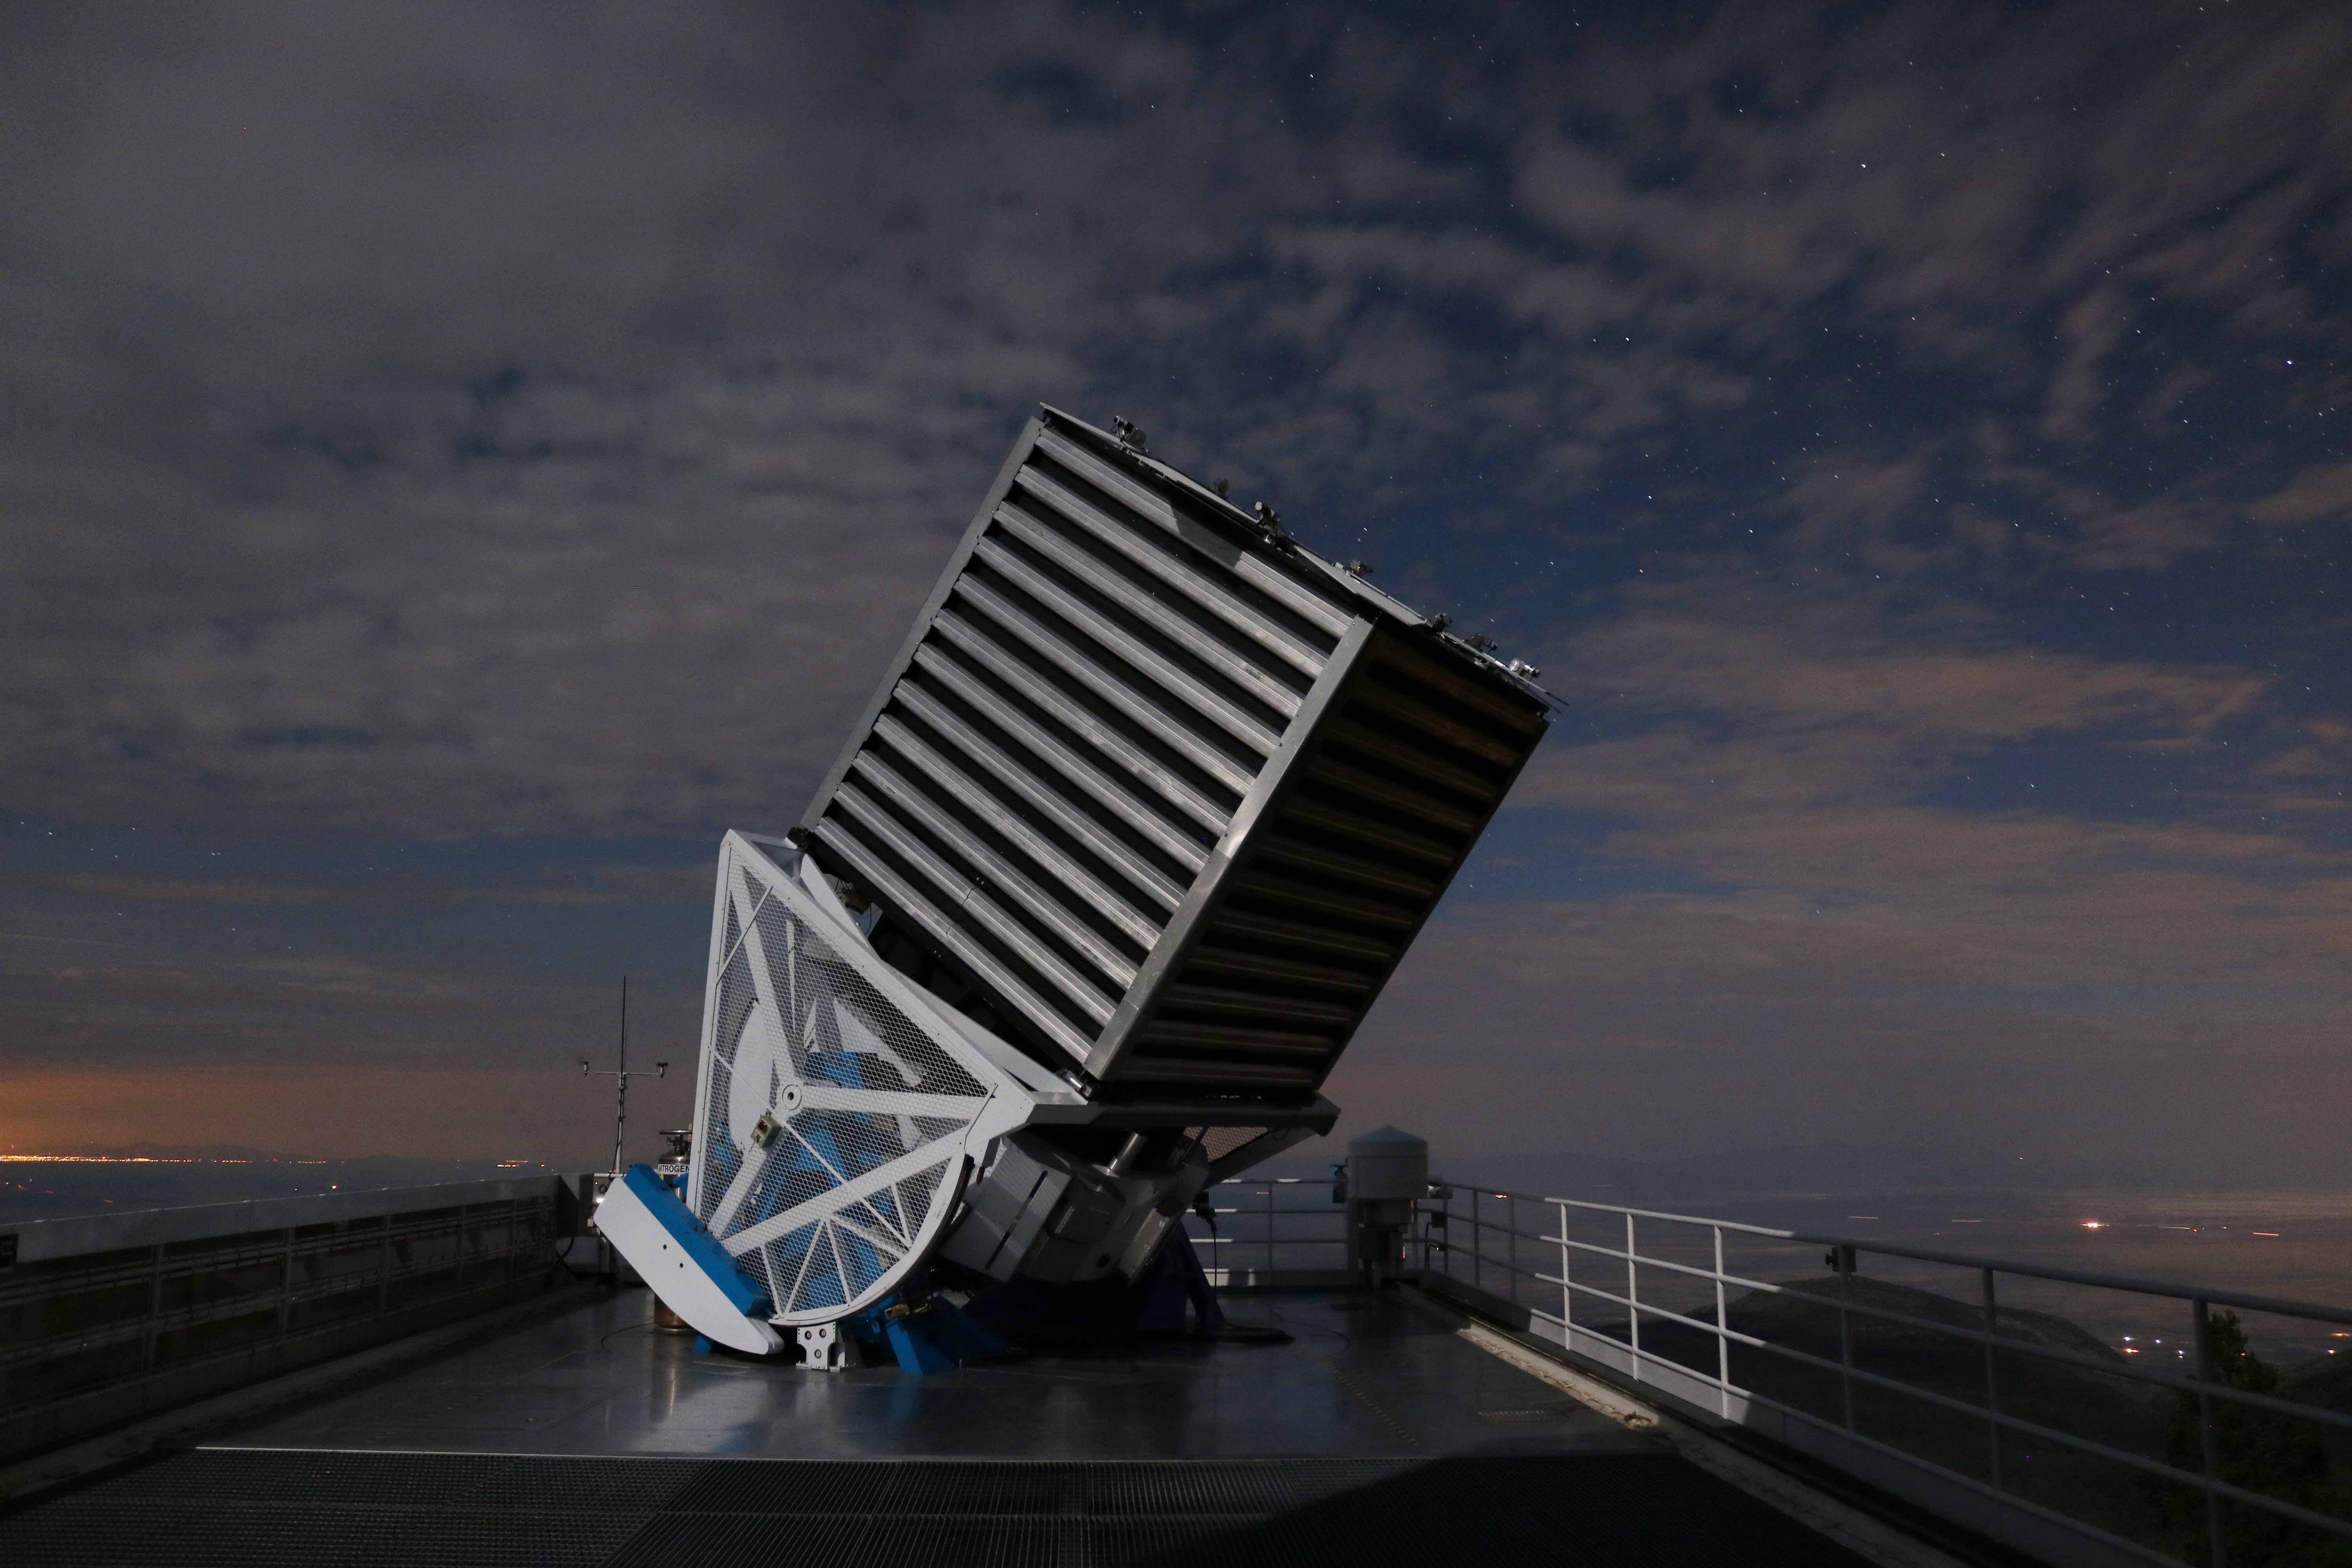
\includegraphics[width=\textwidth]{img/sdss_gaulme.jpg}
\caption[The SDSS telescope]{
	The SDSS telescope at night.
	(Image by Patrick Gaulme is licensed under CC BY 4.0.)
	}
\label{sdss_telescope}
\end{figure}

In 2009, the original spectrograph was upgraded for \textit{Baryon Oscillation Spectroscopic Survey} (BOSS).
The upgraded BOSS spectrograph covers a wavelength range 356--1\,040~nm
with resolving power \(R \sim 2\,000\)
and is capable to 1\,000 spectra at once.~\cite{smee2013}

Its recent SDSS Data Release 14 (SDSS DR14) which corresponds to the latest catalog of QSOs
contains more than one-third of the entire celestial sphere.
The total number of optical spectra is 4\,851\,200.

The SDSS Data Release 14 Quasar (SDSS DR14Q) catalog described in~\cite{paris2018}.
The SDSS DR14Q catalog contains 526\,356 quasars (contamination is estimated to be about 0.5\%).
SDSS provides calibrated spectra covering the wavelength range 3\,610--10\,140~\AA{} at a spectral resolution 1\,300 < \(R\) < 2\,500 for all the quasars.

% TODO define luminosity
The catalog defines a quasar is an object with a luminosity \(M_i[z = 2] < -20.5\)
and either displaying at least one emission line with FWHM > 500~km~s\(^{-1}\) or,
if not, having interesting absorption features.

\subsection{Large Sky Area Multi-Object Fiber Spectroscopic Telescope}
\label{lamost}

LAMOST survey was launched in 2012
and has two primary scientific goals to explore both extragalactic
and intragalactic phenomenons.
Therefore, unlike SDSS LAMOST also observes large volume of stars.
However, the other scientific goal of LAMOST is the extragalactic spectroscopic survey of the large scale structure of the universe and the physics of galaxies.
The goal includes spectroscopic survey of nearly 10 millions galaxies and \textit{quasars}
that will contribute to the study of the accretion process of massive black holes in AGNs besides other things.~\cite{cui2012}

The LAMOST is located in Xinglong Station of national Astronomical Observatory, China.
The telescope is a special telescope with a primary mirror made of 37 hexagonal spherical mirros of total size 6.67~m times 6.05~m.
The large primary mirror makes the field of view of 5\(^{\circ}\).
The focal surface has 4\,000 fibers connected to 16 spectrographs with 32 CCD cameras.
Therefore, the telescope is capable of observing up to 4\,000 spectra simultaneously
in a wavelength coverage of 370--900~nm with spectral resolution \(R = 1\,000\) or \(R = 1\,500\) depending on gratings and camera positions.~\cite{cui2012}

LAMOST Data Release 5 v3 (LAMOST DR5) released in June 2019
contains 9\,026\,365 optical spectra.
LAMOST released three catalogs of QSOs
(DR1~\cite{ai2016}, DR2\&3~\cite{dong2018} and DR4\&5~\cite{yao2019})
that in total contains 42\,552 spectra of QSOs.

\subsection{Comparison of the Spectral Data}

Now, we compare the SDSS and LAMOST survey
to prove their suitability for domain adapation.
The surveys are mainly different in term of instruments, sky coverage and target strategy.

Concerning the instrument we summarise the main parameters of telescopes
of the surveys in Table~\ref{telescopes_parameters}.
We see that LAMOST has lower resolution and shorter wavelength coverage than SDSS.
However, SDSS has smaller field of view.

\begin{table}
\begin{center}
\begin{tabular}{|l|r|r|r|}
	\hline
	Parameter of a telescope & SDSS & BOSS & LAMOST \\
	\hline \hline
	Wavelength coverage (nm) & 380--920 & 356--1\,040 & 370--900 \\ \hline
	Spectral resolution \(R\) & 1\,800 & 2\,000 & 1\,250 \\ \hline
	Field of view & \multicolumn{2}{|c|}{3\(^{\circ}\)} & 5\(^{\circ}\) \\ \hline
\end{tabular}
\end{center}
\caption{Parameters of telescopes}
\label{telescopes_parameters}
\end{table}

Sky coverage is very connected to the targeting strategy or scientific goals.
Figure~\ref{sky_coverage} displays sky coverage of both SDSS and LAMOST.
We see that SDSS does not observe our Milky Way galaxy.
On the other hand LAMOST observes everywhere on the notrh hemisphere
but is not able to obserce close to zenit due to its construction limits.

From the perspective of coverage of QSOs depicted in Figure~\ref{qso_coverage}
LAMOST did not observe QSOs in some part of sky
where QSOs are abundant according to SDSS.

% TODO 90 is not complete in charts
\begin{figure}
\begin{center}
\subfloat[][]{
	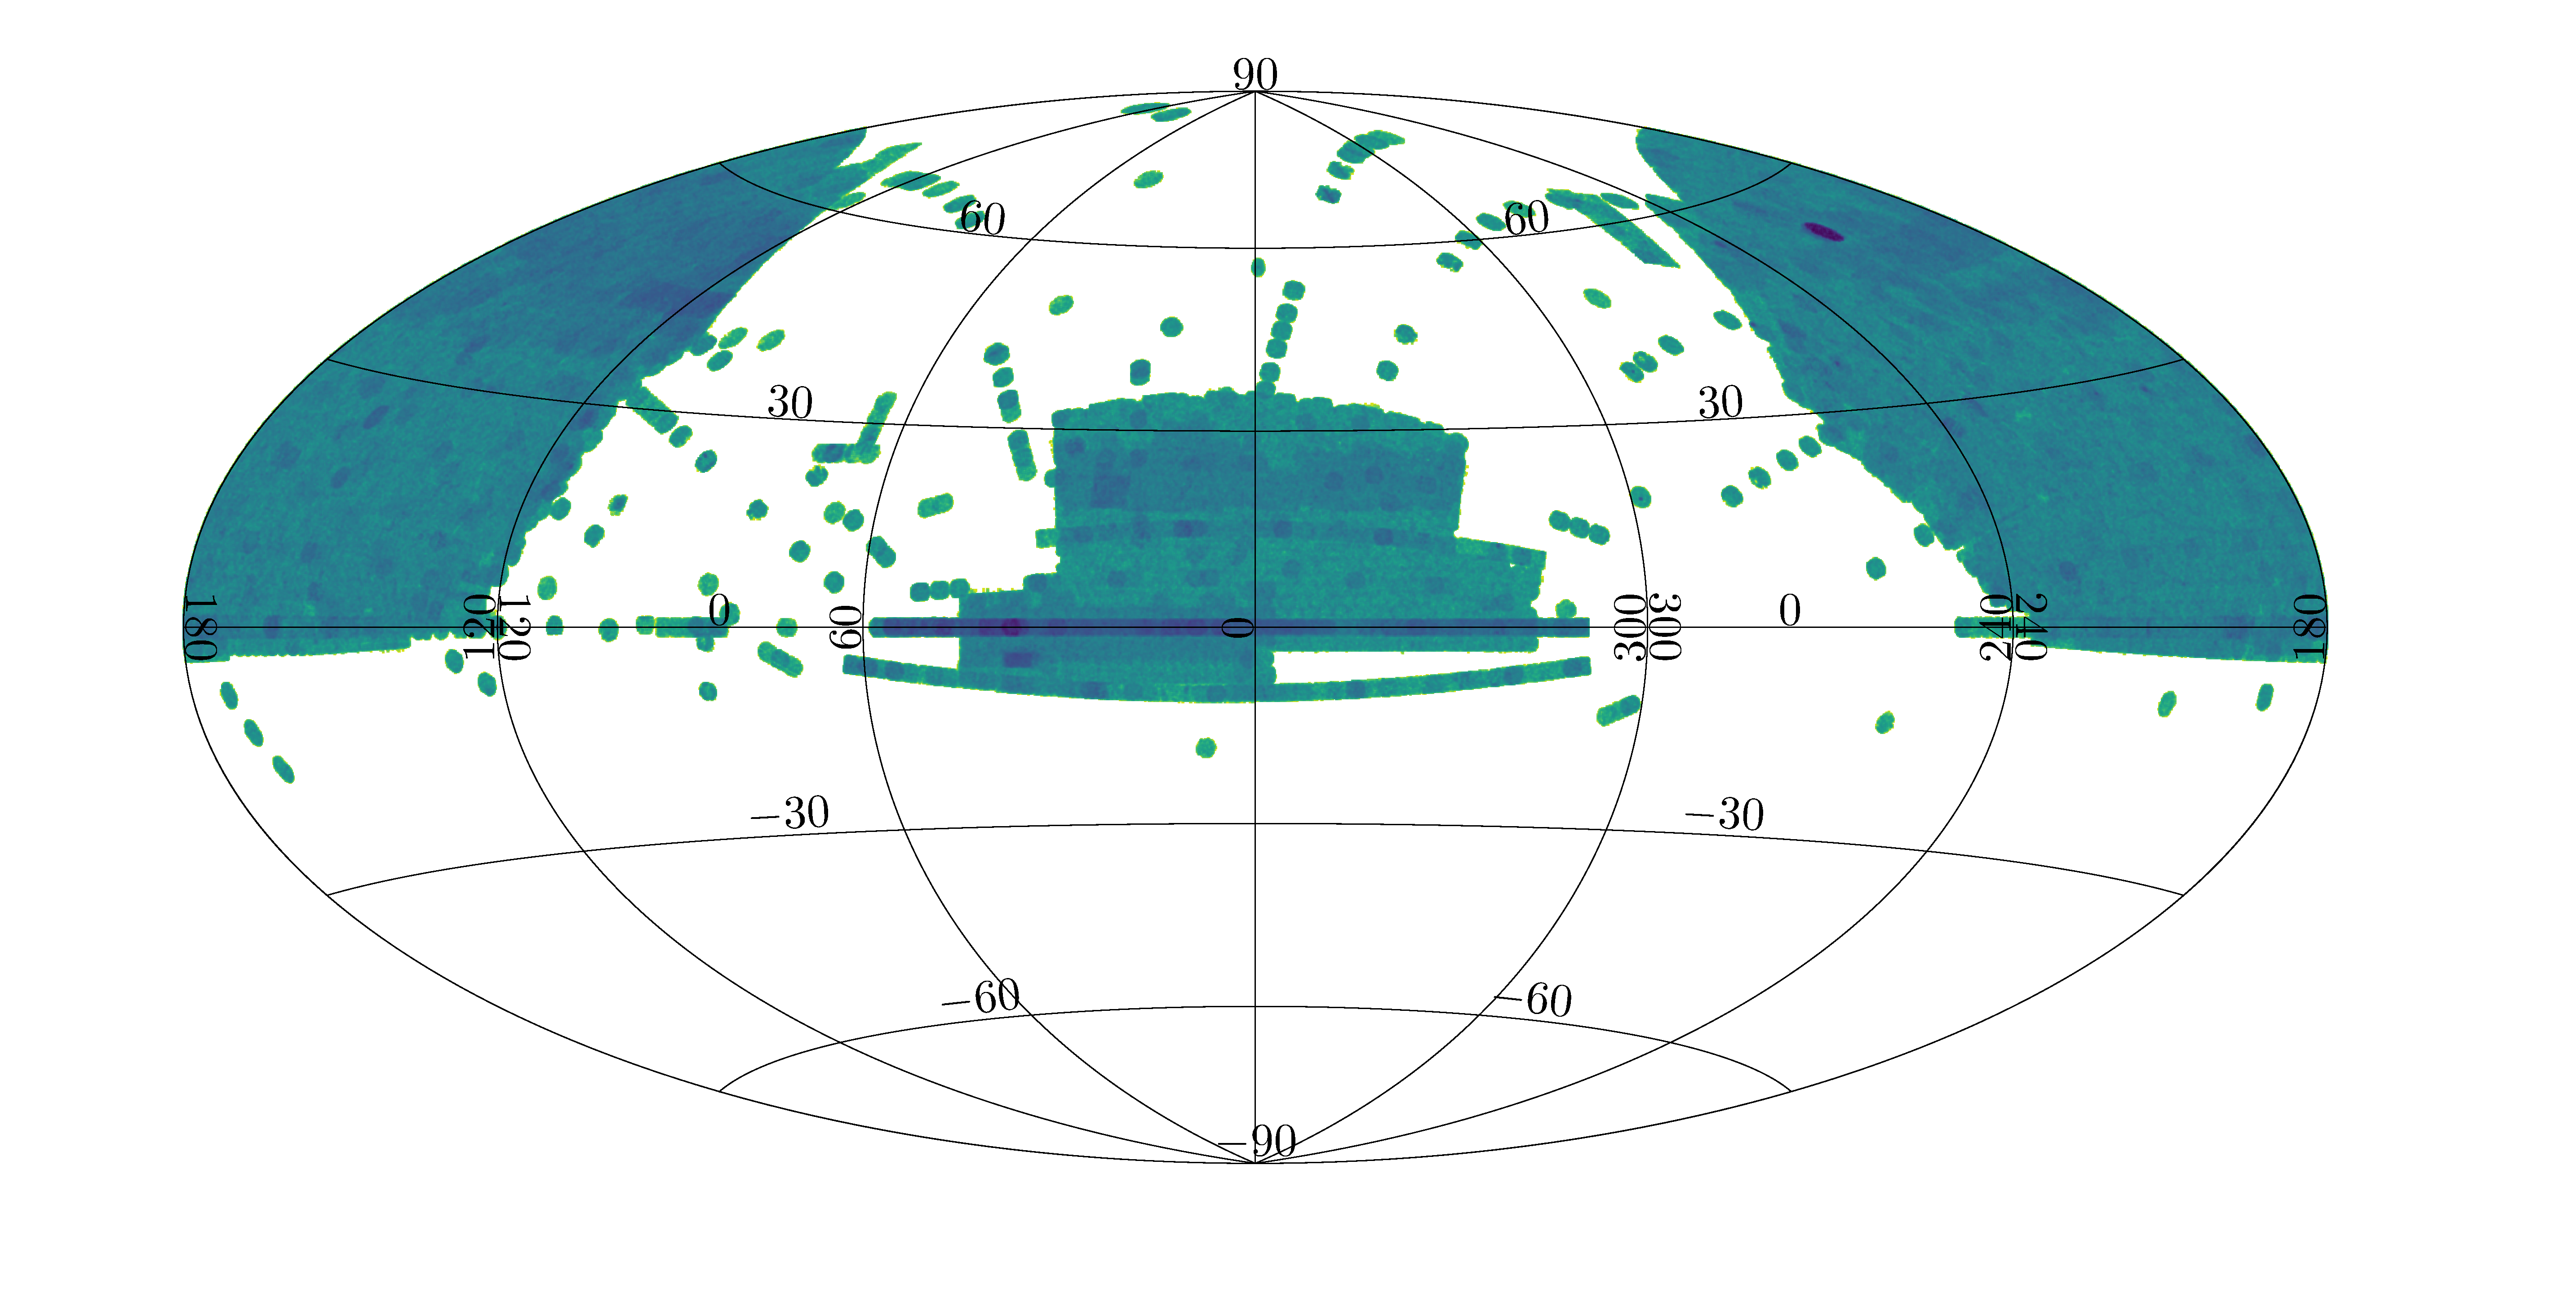
\includegraphics[width=\textwidth]{img/sdss.pdf}
}\\
\subfloat[][]{
	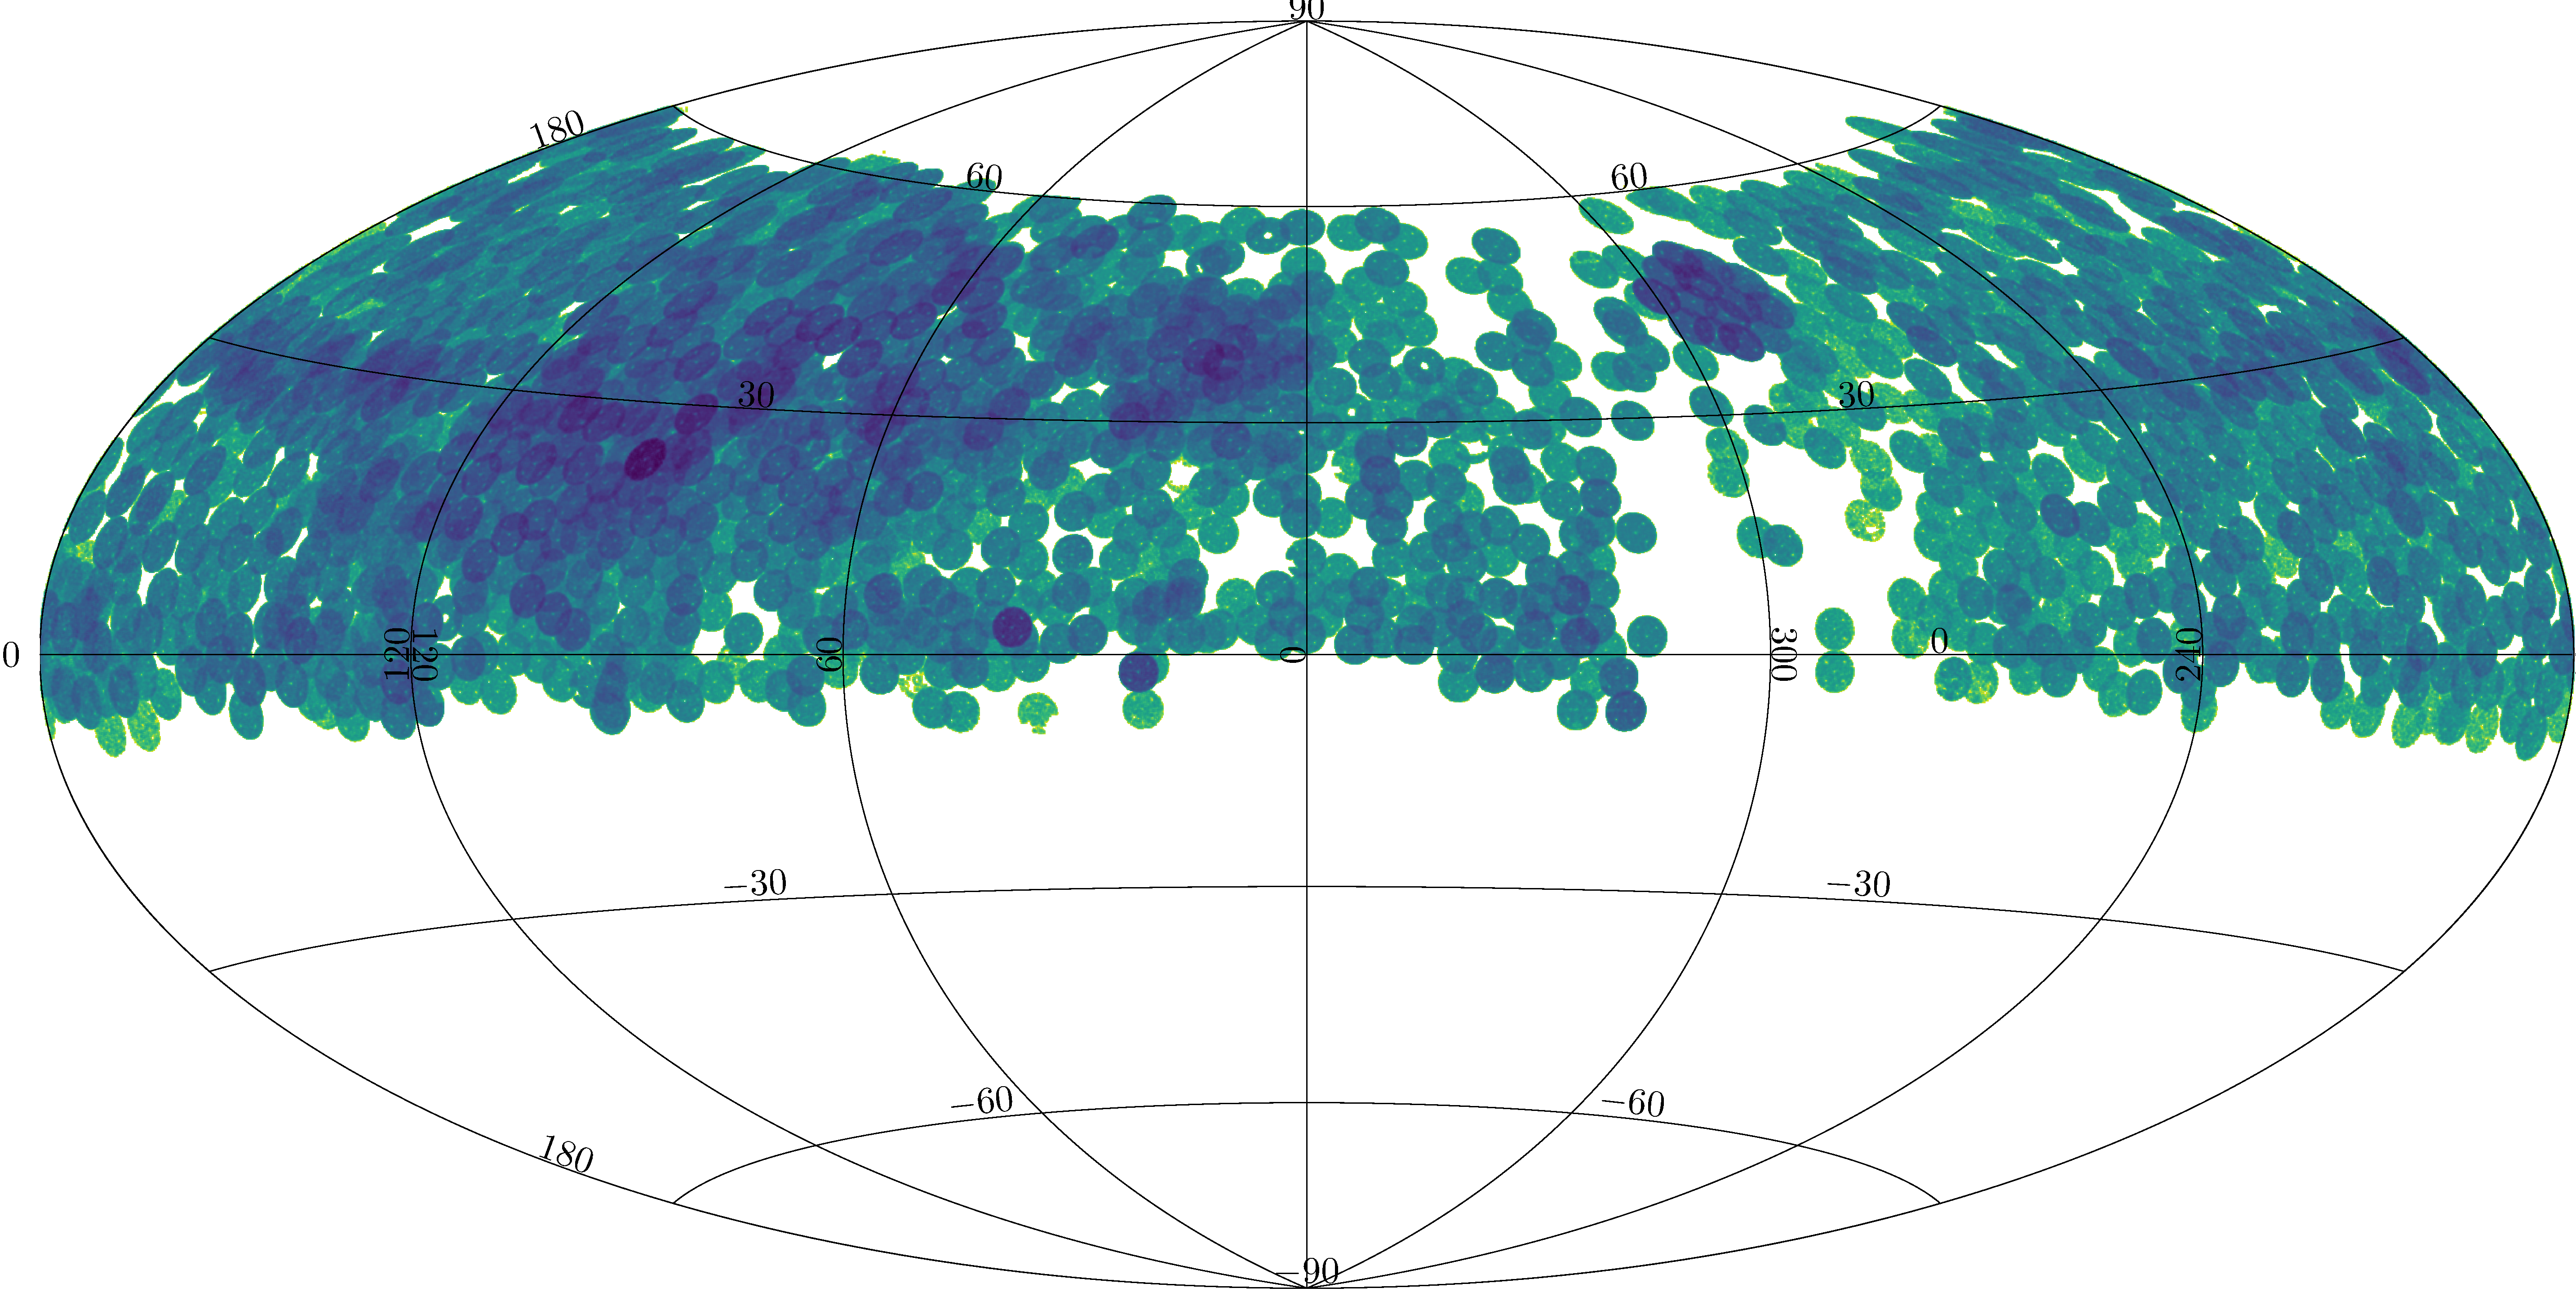
\includegraphics[width=\textwidth]{img/lamost.pdf}
}
\end{center}
\caption[Sky coverage of SDSS and LAMOST]{}
\label{sky_coverage}
\end{figure}

\begin{figure}
\begin{center}
\subfloat[][]{
	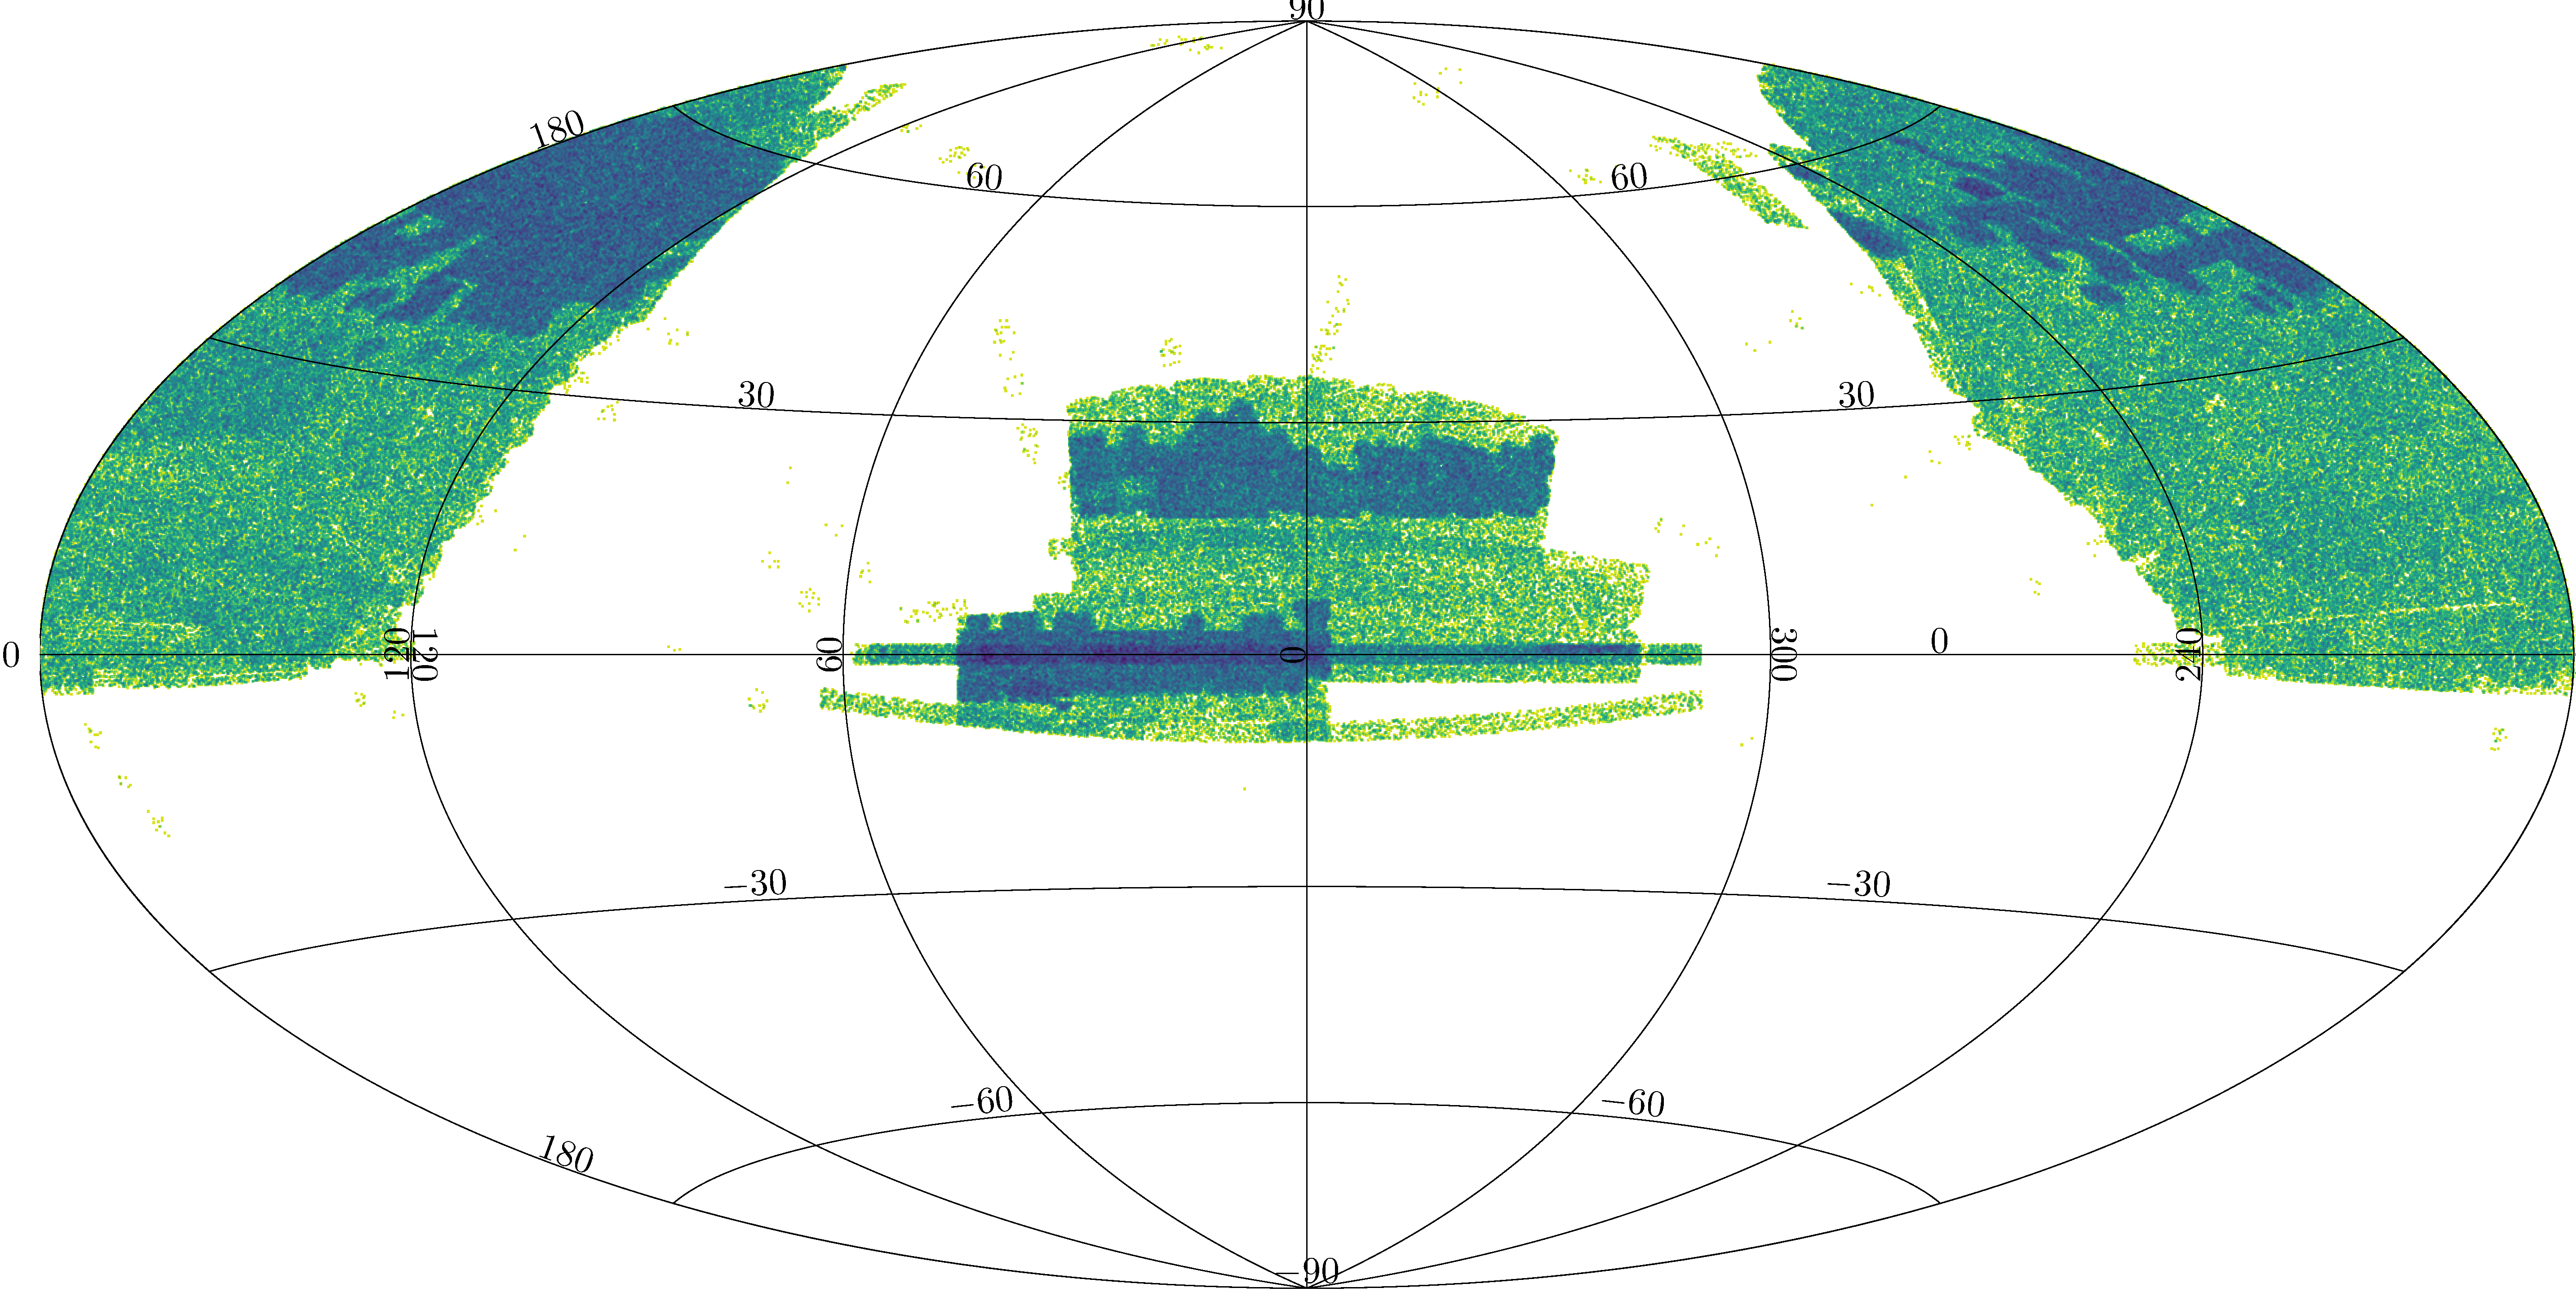
\includegraphics[width=\textwidth]{img/sdss_qsos.pdf}
}\\
\subfloat[][]{
	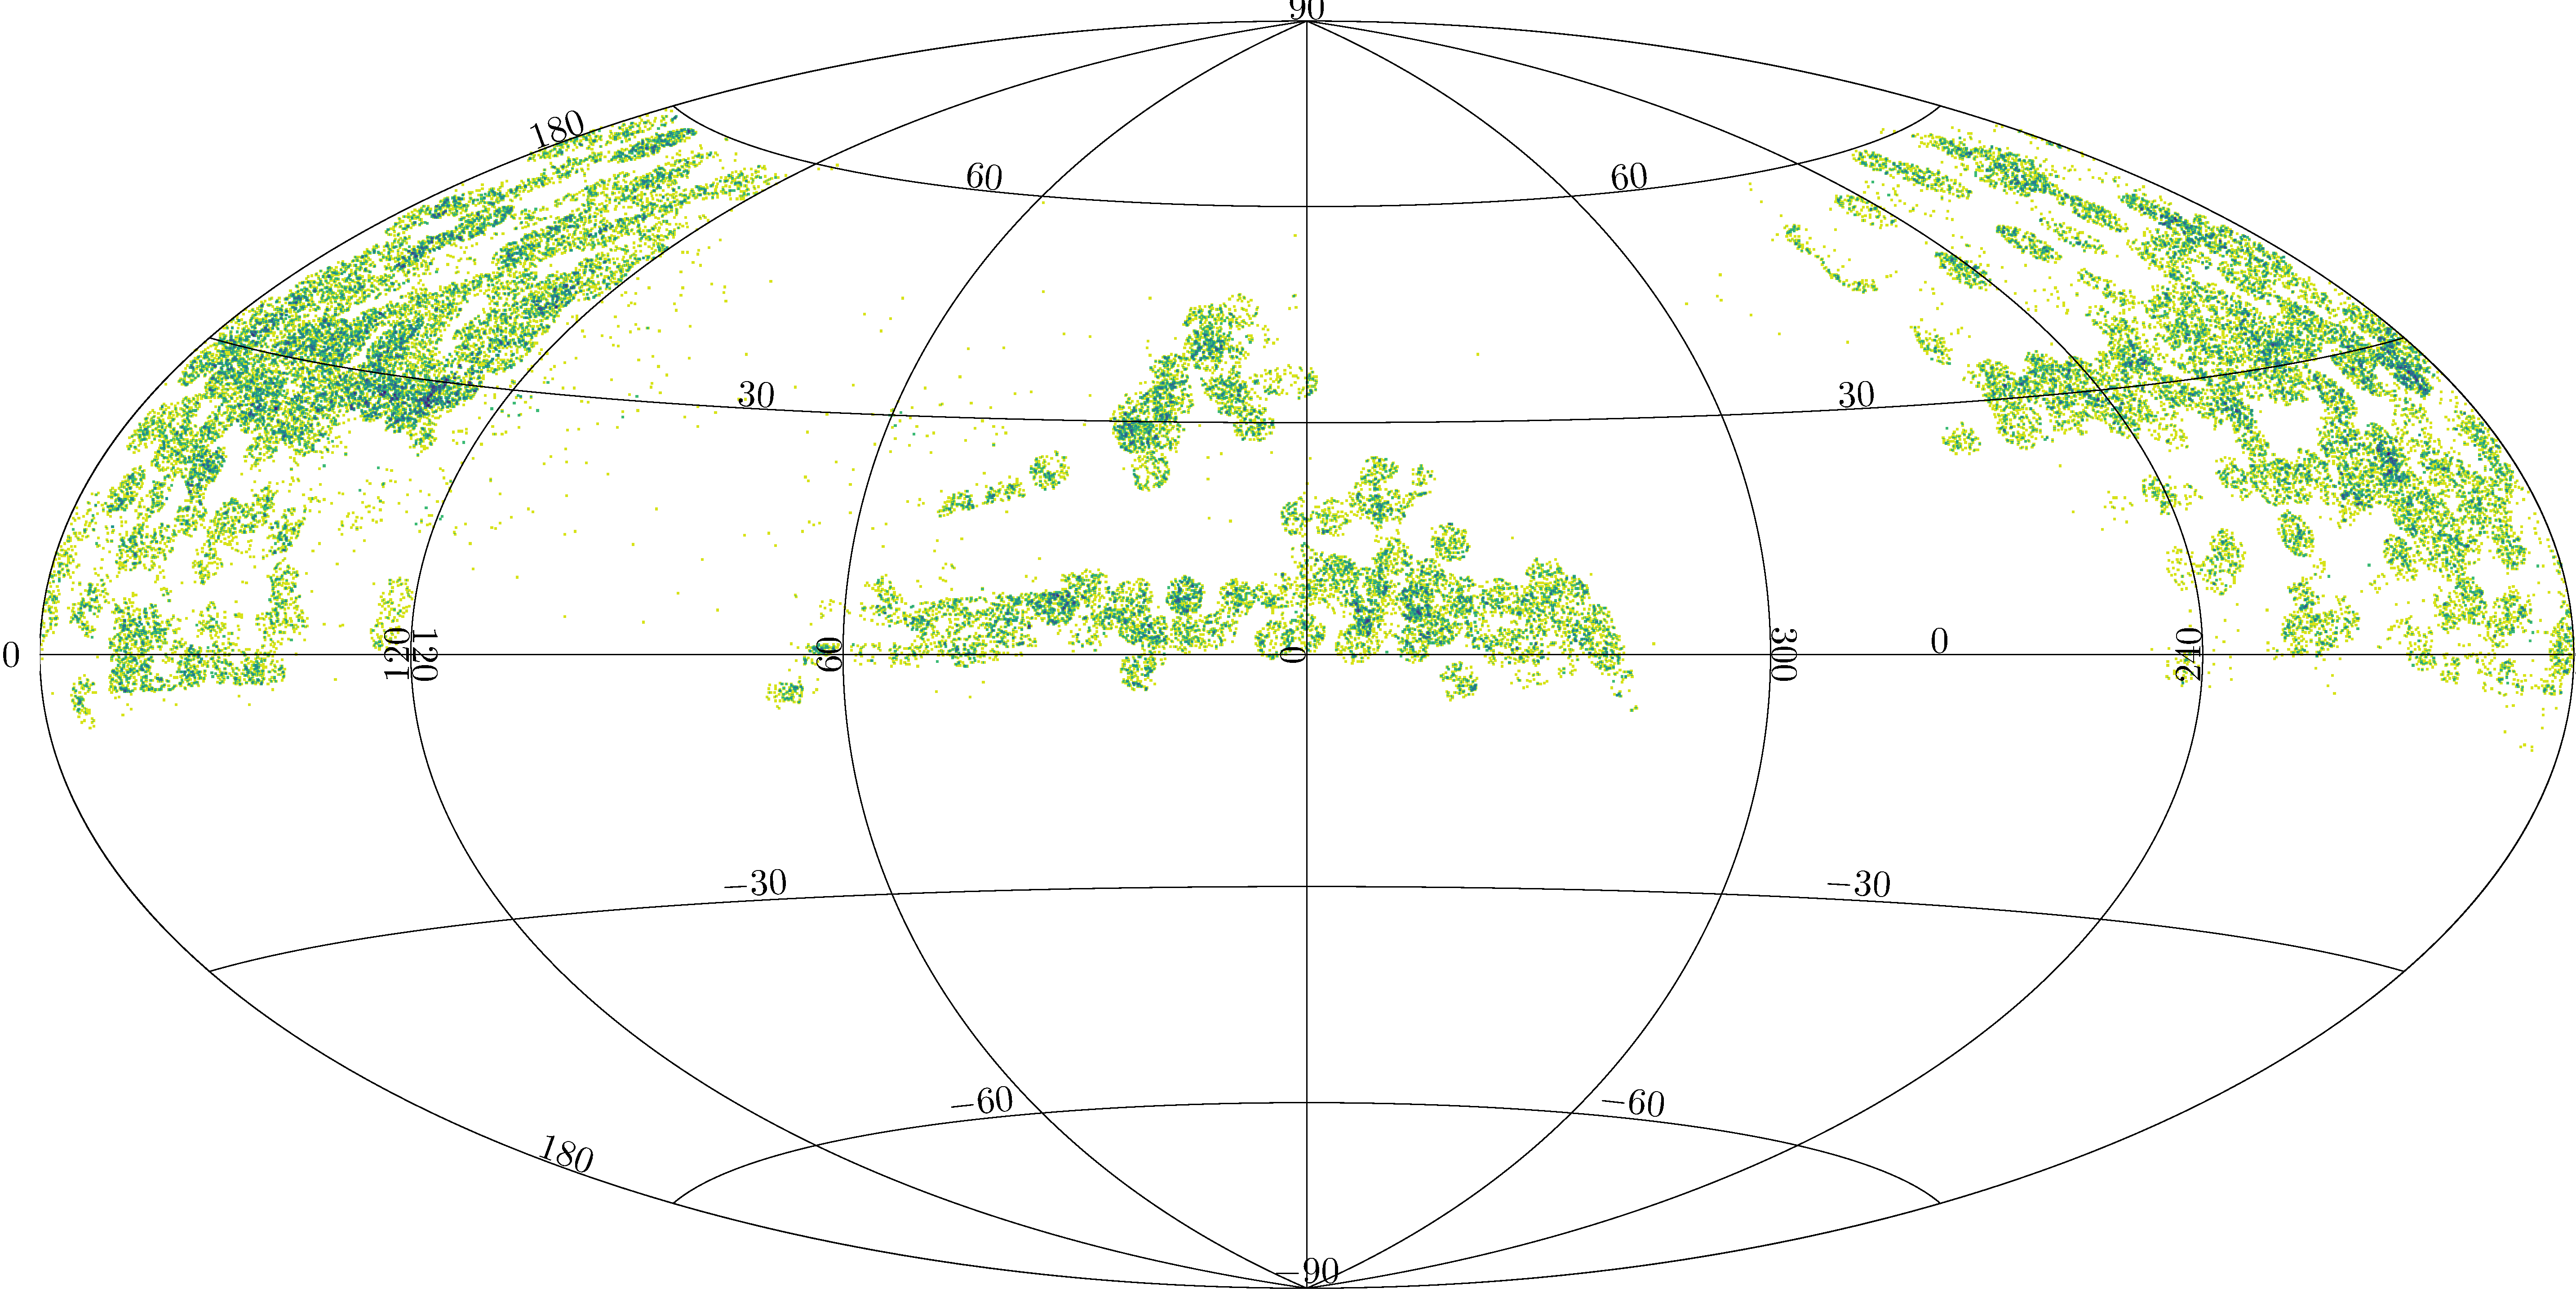
\includegraphics[width=\textwidth]{img/lamost_qsos.pdf}
}
\end{center}
\caption[QSOs coverage of SDSS and LAMOST]{}
\label{qso_coverage}
\end{figure}

We conclude that the two surveys seems to be suitable for domain adatpation
because their instrument create spectra with different resolution
and wavelegth range.
Moreover, observations of SDSS and LAMOST survey has different distribution.

\chapter{Domain Adaptation (DA)}
\label{da_chapter}

Survey the current state of domain adaptation using neural network models in machine learning and with a focus on astronomical applications.

% TODO include examples from astronomical spectroscopy

\section{DA in Context of Machine and Transfer Learning}

Now, we introduce the crucial concept of our work: domain adaptation.
Domain adaptation is a subfield of transfer learning,
which is part of machine learning.
Transfer learning is defined in most papers regarding the survey by Pan and Yang~\cite{pan2010}.
A more recent survey by Weiss, Khoshgoftaar and Wang~\cite{weiss2016} has the benefit
that it contains newer methods than the survey by Pan and Yang~\cite{pan2010},
but its definition of transfer learning and domain adaptation is the same.

Machine learning has a common assumption that training and test data are independent and identically distributed
that means samples are drawn from the same feature space and the same distribution.~\cite{daume2006}
When this assumption does not hold transfer learning and domain adaptation come into play.
Moreover, there is a biological inspiration
because humans seem to have natural ways to transfer knowledge from previous experience to new challenges.~\cite{torrey2010}

% TODO define TL
Pan and Yang~\cite{pan2010} define transfer learning
as the ability of a system to recognise and apply knowledge and skill
learned in previous tasks to novel tasks
and they introduce the notion of a domain and a task.

A domain consists of two components: a feature space and a marginal probability distribution.

\begin{definition}
	A domain \(\mathcal{D} = [X, P(X)]\)
	is a~\(d\)-dimensional feature space \(X \subset \mathbb{R}^d\)
	with a~marginal provavility distribution \(P(X)\).~\cite{pan2010}
\end{definition}

Given a specific domain, a task consists of two components: a label space and an objective predictive function
which is not observed but learned from training data.

\begin{definition}
	A task \(\mathcal{T} = [Y, P(Y | X)]\)
	is a label space \(Y\)
	and a conditional probability distribution \(P(Y | X)\).~\cite{pan2010}
\end{definition}

When we are given a transfer learning problem,
we have to identify a source domain and a source learning task,
a target domain and a target learning task.
Then, transfer learning aims to help improve the learning of the target predictive function in the target domain using knowledge in the source domain and the source task,
where the domains are different or the tasks are different.~\cite{pan2010}

Lastly, Torrey and Shavlik warn that both the source and target domains and tasks need to be sufficiently related
else negative transfer may occur.
Negative transfer is the situation in which the usage of source data degrades the performance.
On the other side, when the performance is improved,
we talk about a positive transfer.~\cite{torrey2010}

TL helps to exploit data or models available in similar domains.~\cite{csurka2017}

\section{Theory and Formalization of DA}

% TODO define DA
Domain adaptation (DA) is a particular case of TL
that leverages labelled data from source domain to learn a classifier for a target domain while the tasks are the same.
It is assumed that source and target domains are not identical but related.
If they were identical it would be a standard machine learning problem.
Therefore there is a distribution discrepancy between the source and target domains (\textit{domain shift}).~\cite{csurka2017}

\begin{definition}
	\textit{Domain adapatiton} is the scenario when the source
	\(\mathcal{D}^s = [X^s, P(X^s)]\)
	and target \(\mathcal{D}^t = [X^t, P(X^t)]\)
	are different (\(\mathcal{D}^s \ne \mathcal{D}^t\))
	but the source \(\mathcal{T}^s\) and target \(\mathcal{T}^t\)
	tasks are the same (\(\mathcal{T}^s = \mathcal{T}^t\)).
	% TODO should be the second condition always true for DA
	The first condition implies \(X^s \ne X^t\),
	\(P(X^s) \ne P(X^t)\) or both are true.~\cite{pan2010}
\end{definition}

% TODO refer to specific section
In our case, the two archive have different target selection strategies
and the instrument are different.

\begin{definition}
	\textit{Homogeneous} DA is setting in which the source \(X^s\)
	and target \(X^t\) feature spaces are the same
	(\(X^s = X^t\))
	while in \textit{heterogeneous} the source and target spaces are different
	(\(X^s \ne X^t\)).~\cite{csurka2017}
\end{definition}

% TODO check feature space
Our case is the \textit{homogeneous} DA where the feature spaces are identical
(\(X^s = X^t\))
still the source and target data are have different distributions
(\(P(X^s) \ne P(X^t)\)).
Therefore, further we focus on homogeneous DA.
because our spectra prepared into a same feature space (\(\mathbb{R}^{3659}\)).

Next we distinguish \textit{supervised}, \textit{semi-supervised}
and \textit{unsupervised} DA
according to availability of labels in the target domain:

\begin{itemize}
	\item superivesed DA: labelled data in the target domain are present;
	\item semi-supervised DA: we have only very limited amount of labelled data in the target domain while most of the data is unlabelled;
	\item unsupervised DA: no labelled data are available in the target domain.
\end{itemize}

We are concern with \textit{unsupervised DA} because we have
% TODO refer to a section
no reliable labelled data in the target domain.~\cite{wang2018}
In corespondence with~\cite{ganin2016},
we consider a classification problem within an input space \(X\)
with \(L\) possible labels from a set \(Y = {0, \dots, L - 1}\).
The source \(\mathcal{D}_s\) and target \(\mathcal{T}_s\) domains
have different distibutions over \(X \times Y\).
From the source and target domains
we have \textit{labelled source sample} \(S\) drawn i.i.d. from \(\mathcal{D}_s\)
and \textit{unlabelled target sample} \(T\) drawn i.i.d. from \(\mathcal{D}^X_t\) 
(the marginal distribution of \(\mathcal{D}_t\) over \(X\)):

\begin{align}
	S &= \{(\mathbf{x}_i, y_i)\}^n_{i = 1} \sim (\mathcal{D}_s)^n, \\
	T &= \{\mathbf{x}_i\}^N_{i = n + 1} \sim (\mathcal{D}^X_t)^{n'},
\end{align}

where \(N = n + n'\) is the total number of examples (data points).

Nowadays, methods of DA are generally distinguished into to categories:
\textit{shallow DA} methods that can be applied on extracted vectors of features
and \textit{deep DA} methods based on neural networks and deep learning
augemented for domain adapation.~\cite{csurka2017}

According to Wang and Deng~\cite{wang2018} shallow DA methods
can be categorised into two classes:
\textit{instance-based DA}
(the discrepancy is reduces by reweighting the source instances)
and \textit{feature-based DA}
(tries to learn a common shared space in which the discrepancy diminishes).
However, shallow DA methods are not interesting for us
because they do not utilize neural network.
Still one possibility is to use a neural network as a feature extractor.~\cite{csurka2017}

The following section introduces the other category of deep DA
which takes the advantage of neural networks.

\section{Previous Applications of DA in Astronomy}

% TODO something like: so far shallow but some deep DA not sufficient

As we have shown, domain adaptation is of great interest to astronomers
because of different instruments, measurements and observation distribution.
Therefore, we survey the current state of domain adaptation in astronomical applications in this section.

If we have a common set of observed stars in both archives,
then we can map them and learn a transfer function.
Ho et al.~\cite{ho2017} did exactly that
% TODO add APOGEE to acronyms
because they found a common set of 9\,952 spectra in both APOGEE and LAMOST archive.
Using that set, they trained the Cannon method~\cite{ness2015},
and they used the model to transfer some physical parameters from APOGEE to LAMOST.

In the case, when there is no common set Gupta et al. experimented with subspace alignment~\cite{fernando2014} and kernel mean matching~\cite{gretton2009} followed by active learning.~\cite{gupta2016}
In the case of subspace alignment, the negative transfer occurred while the kernel mean matching seems very promising in the task of supernova classification.
Then, Vilalta et al.~\cite{vilalta2018} extended the work of Gupta et al.~\cite{gupta2016}.
Vilalta et al. used a maximum a posteriori (MAP) approach to learn a prior on the model parameters from a spectroscopic source domain
and then use this prior distribution to learn a model in a photometric target domain.
Concretely, Vilalta et al. put a prior on the number of layers of a neural network
and then used active learning.
Richards et al.~\cite{richards2011} faced a similar situation, as Gupta et al.
Richards et al. introduce the problem as sample selection bias~\cite{shimodaira2000} or covariate shift~\cite{heckman1979}
when different distributions generate the source and target data.
That is precisely the problem we have defined as domain adaptation.
Richards et al. experimented with random forest in combination with three domain adaptation methods:
importance weighting~\cite{shimodaira2000}, co-training~\cite{blum1998} and active learning~\cite{settles2009}.
The result is not surprising from our point of view.
Active learning works best while importance weighting and co-training achieve negative transfer.

The term transfer learning has been recently used in the context of deep learning.
However, transfer learning in the context of deep learning means something more concrete than what we defined as transfer learning previously.
Transfer learning in the context of deep learning is the specific situation
when a pretrained deep neural network model is taken,
and its last layers are retrained with the target domain data.
Ackermann et al.~\cite{ackermann2018} employed with the transfer learning approach in the context of deep learning to detect galaxy merges.
Ackermann et al. took the Xception convolutional neural network~\cite{chollet2017}
and retrain its last layers with images of galaxy merger labelled in a citizen science Galaxy Zoo project.
This transfer learning approach allowed Ackermann et al. to lower the best error rate so far by 15\%.

\section{Neural Networks in DA}

Donahue et al. showed in the paper on DeCAF~\cite{donahue2014}
that deep neural networks learn more transferable features
but the performance is still affected by the domain shift.

% TODO write about DeCAF

The group of DA methods using neural networks is called \textit{deep DA}
and Wang \& Deng define it in~\cite{wang2018}:

% TODO broad and narrow sense
\begin{definition}
	Deep DA is a method that utilizes a deep network to enhance the performance of DA.
\end{definition}

Approaches to deep DA were originally divided by Csurka in~\cite{csurka2017}
into three categories according to training loss.
Then, Wang and Deng further improve and detail the categorisation in~\cite{wang2018}:

\begin{itemize}
	\item \textit{discrepancy-based} DA fine-tunes the neural network
		with target data to diminish the domain shift;
	\item \textit{adversarial-based} DA encorage domain confusion
		by using discriminators with adversarial objective; and
	\item \textit{reconstruction-based} DA uses data reconstruction auxialiary task to learn domain invariant features.
\end{itemize}

We summarize the deep DA methods categorisation in the mind map of Figure~\ref{mind_map}.

\begin{figure}
	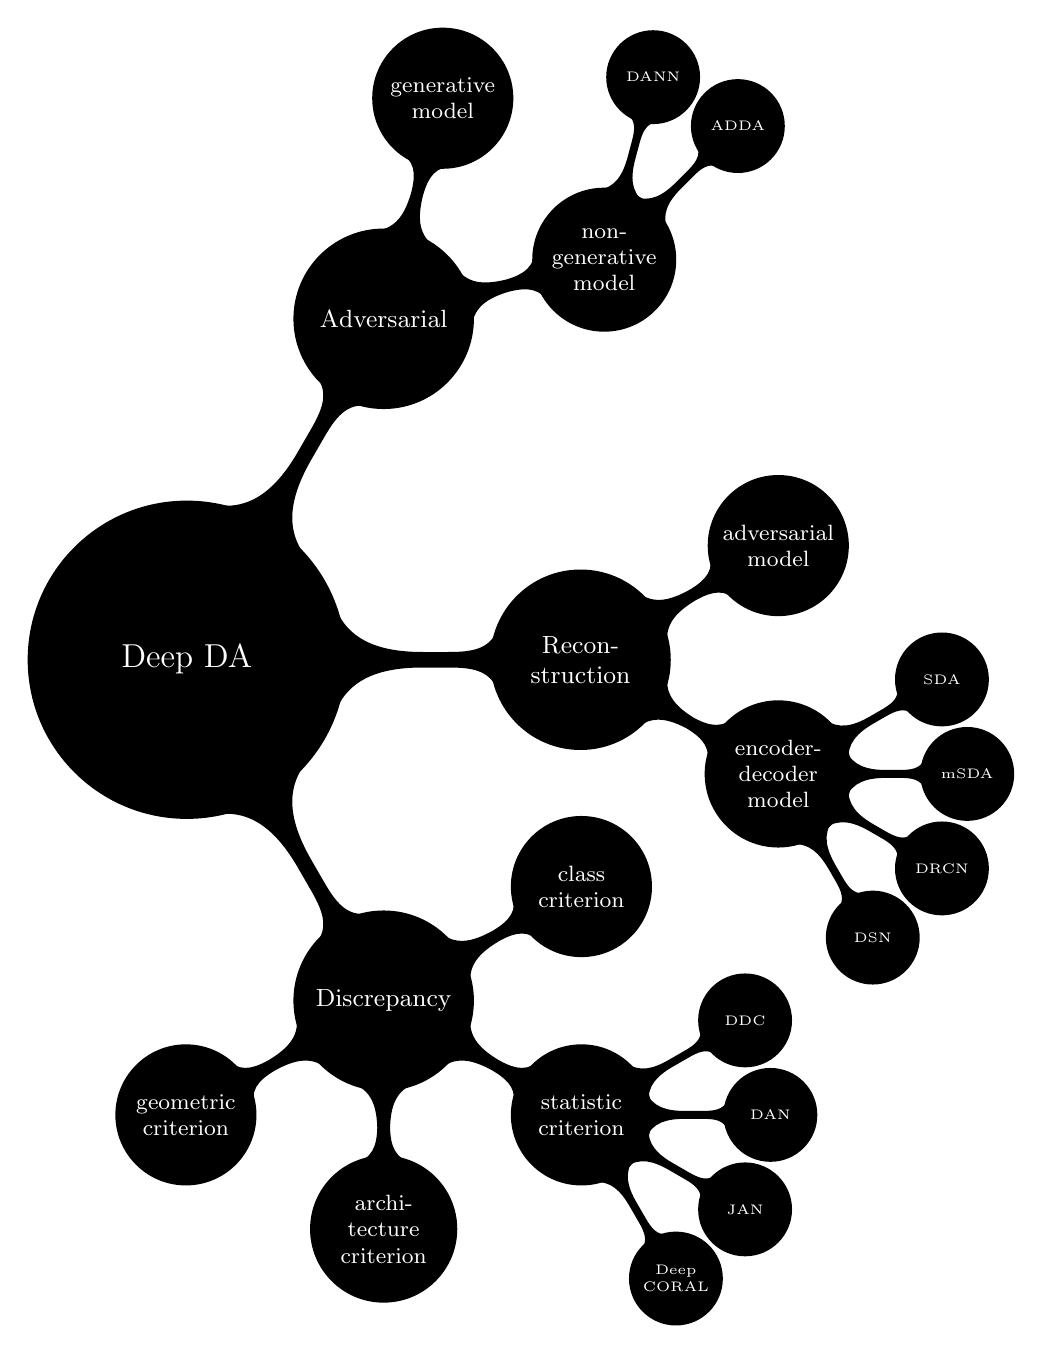
\begin{tikzpicture}
		\path[mindmap, concept color=black, text=white]
		node[concept] {Deep DA}
		[clockwise from=60]
		child[concept] {
			node[concept] {Adversarial}
			[clockwise from=75]
			child {node[concept] {generative model}}
			child {
				node[concept] {non-generative model}
				child {node[concept] {DANN}}
				child {node[concept] {ADDA}}
				}
			}
		child[concept] {
			node[concept] {Recon\-struction}
			[clockwise from=30]
			child {node[concept] {adversarial model}}
			child {
				node[concept] {encoder-decoder model}
				child {node[concept] {SDA}}
				child {node[concept] {mSDA}}
				child {node[concept] {DRCN}}
				child {node[concept] {DSN}}
				}
			}
		child[concept] {
			node[concept] {Discrepancy}
			[clockwise from=30]
			child {node[concept] {class criterion}}
			child {
				node[concept] {statistic criterion}
				child {node[concept] {DDC}}
				child {node[concept] {DAN}}
				child {node[concept] {JAN}}
				child {node[concept] {Deep CORAL}}
				}
			child {node[concept] {archi\-tecture criterion}}
			child {node[concept] {geometric criterion}}
			};
	\end{tikzpicture}
	\caption{Mind map of deep DA}
	\label{mind_map}
\end{figure}

\subsection{Discrepancy-based DA}

Discrepancy-based deep DA uses either labelled or unlabelled target data
to fine-tune a neural network to diminish the dicrepancy
between the source and target domains.

The discrepancy-based method divided based on
\textit{class}, \textit{statistic}, \textit{architecture} and \textit{geometric}
criterion by~\cite{wang2018}.

DDC~\cite{tzeng2014}, DAN~\cite{long2015}, JAN~\cite{long2017}
and Deep CORAL~\cite{sun2016}.

The essence of Deep Domain Confusion (DCC)~\cite{tzeng2014} is finding domain invariant representation
while learning to predict class labels.
The intuition behind DDC is that learning represenation
that minimises the distance between source and target distributions
then a classifier trains on source labelled data
can be directly applied to the target domain achieving minimal loss in accuracy.
DDC optimises loss function that includes both prediciton error and \textit{domain confusion} loss to learn deep representation.
The invariant deep repsentation is achived by incorporating an adaptation layer
into a deep CNN with a domain confusion loss computed via \textit{maximum mean discrepancy} (MMD).
MMS is a standard distirbution distance metric
witch is empirically approximated as follows:

\begin{equation}
	\mathrm{MMD}(S, T) = \left\|
	\frac{1}{n} \sum_{i = 1}^{n} \phi(\mathbf{x}_i) -
	\frac{1}{n'} \sum_{i = n + 1}^{N} \phi(\mathbf{x}_i)
	\right\|,
	\label{maximam_mean_discrepancy}
\end{equation}

where \(\phi(\cdot)\) is a represenation
that operates on both source \(\mathbf{s}_i \in S\) and target \(\mathbf{t}_i \in T\) data points.
Using the adaptation layer with the domain loss function DDC claims
to learn representation that is both domain invariant
but still offers strong semantic separation.
However, DDC also want to learn representation
that enables to learn a strong classifier.
Therefore is minimizes a loss that incorporates both domain confusion loss and classification loss:

\begin{equation}
	\mathcal{L}_{\mathrm{DDC}} = \mathcal{L}_c(S)
	+ \lambda \mathrm{MMD}^2(S, T),
\end{equation}

where \(\mathcal{L}_c\) stands for classification loss on the labelled source data \(S\).
To control the stregnth of domain confusion DDC introduces the hyperparameter~\(\lambda\)
(DCC uses \(\lambda = 0.25\) in its experiments).

% TODO cite AlexNet and explain what is pre-trained (cite ImageNet)
In experiments DDC, uses \textit{pre-trained} AlexNet with a lower dimensional \textit{bottleneck} adaptation layer
which should regularise the training
and prevent overfitting the source distribution.
The domain confusion loss is placed on the bottleneck adaptation layer.

% TODO cite Office benchmark and maybe describe?
DDC was evaluated of the Office benchmark achieving 81.2\% average accuracy on the target domains.

\subsection{Adversarial-based DA}

Adversarial-based deep DA utilizes a domain discriminator
that tries to distinguish whether a sample comes from source and target domains.
If we are able to confuse the discriminator
we will also achieve domain confusion through the adversarial objective.

The methods are divided into \textit{generative} and \textit{non-generative}
models by~\cite{wang2018}

DANN~\cite{ganin2016} and ADDA~\cite{tzeng2017}.

% TODO cite http://sites.skoltech.ru/compvision/projects/grl/files/paper.pdf
Domain-Adversarial Training of Neural Neural Networks (DANN)~\cite{ganin2016}
is a representation learning approach for domain adaptation.
DANN is based on idea that features for domain adaptation
cannot discriminate between source and target domains
while maintaining discriminative properties for a classification task.
DANN proposes a \textit{gradient reversal layer} (GRL)
that can be incorporated in almost any feed-forward neural network.
Therefore, DANN jointly optimises feature extractor
and two discrimivative classifier.
The first is a label predictor that predicts classes
and a domain classifier tath discriminates between source and target domains.
The feature extractor is trained to minimise the loss of the label classifier
and maximise the loss of the domain classifier.
Thus, domain classifier and feature extractor are learning in adversarial fashion and encourage domain invariant features.
DANN combines feature extractor, label predictor and domain classifier is a single architecture
and can be trained with standard backpropagation learning algorithm.

Let \(G_f(\cdot; \theta_f)\) be the \(D\)-dimensional neural network feature extractor, with parameters \(\theta_f\),
\(G_y(\cdot; \theta_y)\) be the label predictor with parameters \(\theta_y\)
that takes features from \(G_f\) as inputs and output class probabilities
and \(G_d(\cdot; \theta_d)\) be the domain classifier with parameters \(\theta_d\).

Training DANN is optimising prediction loss and domain loss:

\begin{align}
	E(\theta_f, \theta_y, \theta_d) &= \frac{1}{n} \sum^{n}_{i = 1} \mathcal{L}_y(G_y(G_f(\mathbf{x}_i; \theta_f), \theta_y), y_i) \nonumber \\
	&\qquad {} - \lambda \left(\frac{1}{n} \sum^{n}_{i = 1} \mathcal{L}_d(G_d(G_f(\mathbf{x}_i; \theta_f), \theta_d), d_i) \right. \nonumber \\
	&\qquad \left. {} + \frac{1}{n'} \sum^{N}_{i = n + 1} \mathcal{L}_d(G_d(G_f(\mathbf{x}_i; \theta_f), \theta_d), d_i)\right)
\end{align}

by finding the saddle point \(\hat{\theta}_f\), \(\hat{\theta}_y\), \(\hat{\theta}_d\) that satisfy:

\begin{align}
	(\hat{\theta}_f, \hat{\theta}_y)
	&= \operatorname*{arg\,min}_{\theta_f, \theta_y} E(\theta_f, \theta_y, \hat{\theta}_d),\\
	\hat{\theta}_d
	&= \operatorname*{arg\,max}_{\theta_d} E(\hat{\theta}_f, \hat{\theta}_y, \theta_d).
\end{align}

where \(\mathcal{L}_y\) is a classification loss,
\(\mathcal{L}_d\) is a domain loss,
\(\lambda\) is a trade-off hyperparameter
and \(d_i\) is a binary variable:

\begin{equation}
	d_i =
	\begin{cases}
		0 & \quad \text{if } i \in \{1, \dots, n\} \\
		1 & \quad \text{if } i \in \{n + 1, \dots, N\}
	\end{cases}
\end{equation}

The saddle points can be found using gradient updates:

\begin{align}
	\theta_f &\gets \theta_f - \mu \left(
	\frac{\partial \mathcal{L}_y^i}{\partial \theta_f}
	- \lambda \frac{\partial \mathcal{L}_d^i}{\partial \theta_f}
	\right),
	\label{feature_parameters_update} \\
	\theta_y &\gets \theta_y - \mu
	\frac{\partial \mathcal{L}_y^i}{\partial \theta_y}, \\
	\theta_d &\gets \theta_d - \mu \lambda
	\frac{\partial \mathcal{L}_d^i}{\partial \theta_d}.
\end{align}

The previous updates are very similar to SGD.
However, the update~\ref{feature_parameters_update} has substraction in it instead of addition.

DANN overcomes the substruction by incorporating a gradient reversal layer \(\mathcal{R}(\mathbf{x})\) between the feature extrator and domain classifier.
Now, DANN seamlesly works with SGD.
The gradient reversal layer has no parameters
and during forward propagation the GRL acts as identity:

\begin{equation}
	\mathcal{R}(\mathbf{x}) = \mathbf{x}.
\end{equation}

However, in backpropagation it negates the gradient:

\begin{equation}
	\frac{d \mathcal{R}}{d \mathbf{x}} = -\mathbf{I},
\end{equation}

where \(\mathbf{I}\) is identity matrix.

The objective to be optimised with gradient descent:

\begin{align}
	E(\theta_f, \theta_y, \theta_d) &= \frac{1}{n} \sum^{n}_{i = 1} \mathcal{L}_y(G_y(G_f(\mathbf{x}_i; \theta_f), \theta_y), y_i) \nonumber \\
	&\qquad {} - \lambda \left(\frac{1}{n} \sum^{n}_{i = 1} \mathcal{L}_d(G_d(\mathcal{R}(G_f(\mathbf{x}_i; \theta_f)), \theta_d), d_i) \right. \nonumber \\
	&\qquad \left. {} + \frac{1}{n'} \sum^{N}_{i = n + 1} \mathcal{L}_d(G_d(\mathcal{R}(G_f(\mathbf{x}_i; \theta_f)), \theta_d), d_i)\right)
\end{align}

The gradint reversal layer changes the update~\ref{feature_parameters_update}
to version fully compatible with SGD:

\begin{equation}
	\theta_f \gets \theta_f - \mu \left(
	\frac{\partial \mathcal{L}_y^i}{\partial \theta_f}
	+ \lambda \frac{\partial \mathcal{L}_d^i}{\partial \theta_f}
	\right).
\end{equation}

\subsection{Reconstruction-based DA}

The last group of methods is based on data reconstruction auxialiary task.
The reconstructor forces to find a shared representation
of a source and target domains.

According to~\cite{wang2018} subgroups are \textit{encoder-decoder} and
\textit{adversarial} reconstruction.

SDA~\cite{vincent2008, glorot2011}, mSDA~\cite{chen2012}, DRCN~\cite{ghifary2016} and DSN~\cite{bousmalis2016}.

% TODO check and verify
SDA and mSDA were developed for Amazon reviews benchmark textual data
while DRCN and DSN for visual data.
Therefore we focus on DRCN as it is simpler to train than DSN.

Deep Reconstruction-Classification Network (DRCN)~\cite{ghifary2016} is a CNN that learn both
supervised souce labelled classification
and unsupervised target data reconstruction.
Encoder is shared between both task but decoding parameters are separete.
The data reconstruction task is a auxiliary task
supposed to learn good feature representation beneficial for both source and target domain.

\chapter{Experiments with Deep Domain Adaptation}
\label{exp_chapter}

In previous chapters, we have selected suitable astronomical data, surveyed and chosen suitable deep domain adaptation methods. Now, we carry out experiments with the DDC, Deep CORAL, DANN and DRCN on astronomical spectra from the SDSS and LAMOST spectroscopic sky surveys.

Firstly, we create the source and target datasets for experiments. Then, we use PCA, t-SNE and UMAP to reduce the data to two-dimensions, so we can visualise the data and investigate distributions of both the source and target data. Thirdly, we introduce a CNN baseline model which serves as a benchmark for comparison of the performance of the deep domain adaptation methods. Finally, we employ four deep domain adaptation methods and evaluate the adapted results to see if astronomical spectroscopy can benefit from deep domain adaptation.

\section{Data Preparation}
\label{data_preparation}

Our data of source domain consists of 4\,851\,200 optical spectra from the SDSS DR14 catalogue
and the corresponding SDSS DR14Q catalogue of 649\,791 spectra of 526\,356 QSO objects
(we have to distinguish an object and a spectrum
because each astronomical object could be observed multiple times having multiple spectra).
Both catalogues are introduced in~Subsection~\ref{sdss}.
However, 20\,279 spectra of QSOs cannot be identified
% TODO describe the bug in SDSS DR14Q catalogue
because there is a bug in the SDSS DR14Q catalogue.
Therefore, we can identify only 629\,512 spectra of all QSOs.
Next, we need to cross-match the SDSS DR14 and DR14Q catalogues
to merge the data stored in individual FITS files with QSO labels.
The cross-matching is based on a triplet of a \textit{plate number}, a \textit{Modified Julian Date of observation} and a \textit{fibre number}
that is unique to each spectrum.
Additionally to the 20\,279 spectra of QSOs lost due to the bug in the DR14Q catalogue,
we were unable to cross-match 55 QSOs with the SDSS DR14 catalogue.
Therefore, we have 629\,457 spectra of QSOs
for which we have actual data in FITS files and not only metadata in catalogues.

The complement to the source domain in domain adaptation is the target domain.
We selected data from LAMOST DR5 to be target domain data
for reasons described in Subsection~\ref{lamost}.
The LAMOST DR5 general catalogue contains 9\,026\,365 spectra,
and the complete catalogue of QSOs has 42\,552 spectra.
Again, we cross-matched the LAMOST DR5 catalogue and the catalogue of QSOs
according to a quartet of a \textit{plan identifier}, a \textit{local Modified Julian Date} (one less the Modified Julian Date), a \textit{spectrograph identifier} and an \textit{identifier of fibre}.
We were able to cross-match 31\,755 spectra of QSOs with the general catalogue
effectively losing 10\,797 spectra of QSOs.
We believe that LAMOST has sound reasons for not including those spectra in the LAMOST DR5 catalogue.

However, the labels of QSOs from LAMOST are incompatible with labels from SDSS
because the criteria of what is a QSO are different in SDSS and LAMOST
(see Section~\ref{large_spec_surveys}).
For us, the ground truths are labels of SDSS DR14Q catalogue
while the labels of LAMOST serves only for evaluation purposes,
not for training.
% TODO discuss performace metrics
Therefore, there might be spectra truly QSOs in LAMOST
not yet identified by LAMOST biasing our performance metrics.

Having assigned labels of QSOs to individual spectra,
we need to extract the spectra from individual FITS files
because learning of neural networks requires datasets to be in the form of design matrices.
A design matrix contains a different example (a spectrum) in each row.
In contrast, each column of the design matrix corresponds to a different feature
(a measurement of flux in a specific wavelength).~\cite{goodfellow2016}

Fortunately, SDSS and LAMOST spectra have a common wavelength grid in logarithmic wavelengths evenly space by 0.0001.
Although all spectra have a common wavelength grid,
the minimal and maximal wavelengths are different for each spectrum.
Figure~\ref{wavemin_wavemax_hist} displays histograms of minimal and maximal wavelengths of all LAMOST spectra.
In this work, we aim to find QSOs in the LAMOST DR5.
Therefore, we would like to keep as many spectra as possible from the LAMOST~DR5.
To keep all spectra from the LAMOST~DR5,
we have to select wavelength range starting at 3\,839.7244~\AA{} (3.5843 in logarithmic wavelength)
which is the maximum from minimal wavelengths
and ending at 8\,914.597~\AA{} (3.9501 in logarithmic wavelength)
which is the minimum from maximal wavelengths.
The selection gives us a wavelength grid of 3659 logarithmically-spaced wavelengths
(each spectrum is a real vector of~\(\mathbb{R}^{3659}\)).

\begin{figure}
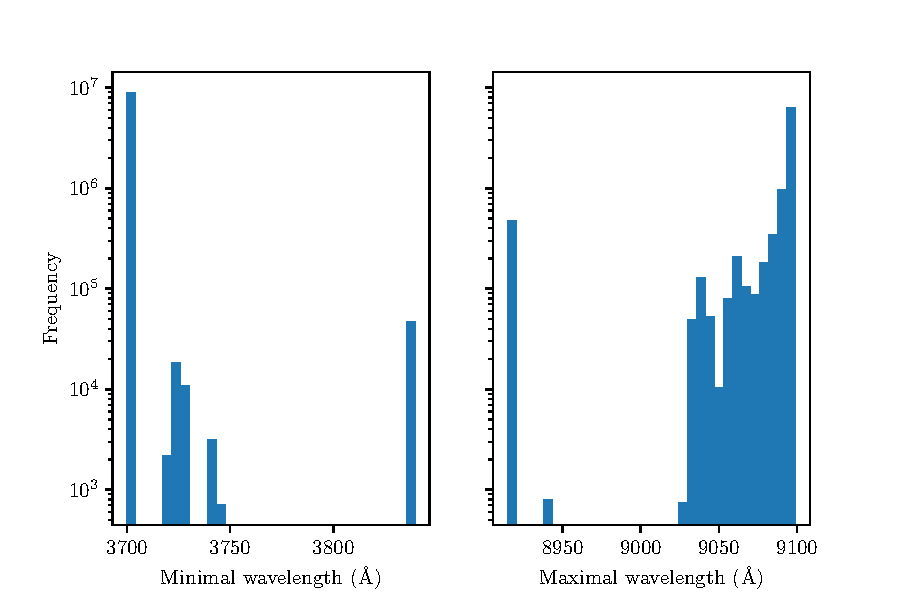
\includegraphics[width=\textwidth]{img/wavemin_wavemax_hist.pdf}
\caption[Minimal and maximal wavelength of LAMOST DR5]{
	Two plots showing histograms of minimal and maximal wavelengths
	of all LAMOST spectra.
	The maximal wavelength from all the minimal wavelengths
	is 3\,839.7244~\AA{}.
	Cutting in lower wavelength
	would mean a lost of almost 100\,000 spectra.
	The situation is very similar for maximal wavelengths
	where the minimum is 8\,914.597~\AA{}.
	Therefore, the most suitable range of wavelength is to choose
	these two wavelengths as starting and ending points.
	}
\label{wavemin_wavemax_hist}
\end{figure}

Given the selected grid of wavelengths,
we will lose some SDSS spectra because not all of them have all measurements in the range.
Figure~\ref{waves_cumulative_hist} shows the cumulative histogram of how many spectra we will keep for cuts in different wavelengths.
We see that significant drops are behind the selected minimal and maximal wavelengths
that mean we will keep most of the spectra.
Precisely, the cut will drop 34\,487 spectra from our source dataset
including 1\,949 spectra of QSO.
Therefore, the source dataset has 4\,816\,713 spectra with 627\,508 spectra of QSOs that can enter learning of a neural network.

\begin{figure}
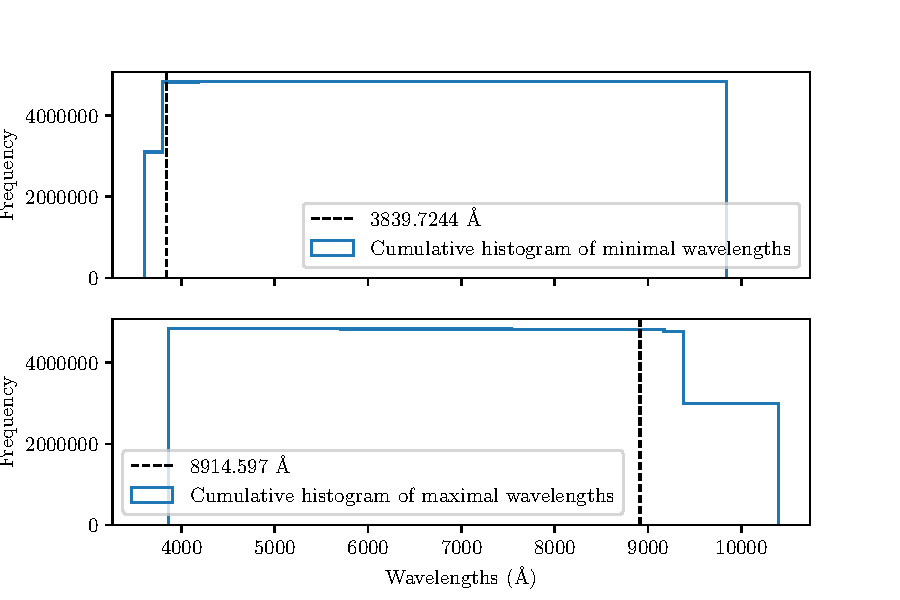
\includegraphics[width=\textwidth]{img/waves_cumulative_hist.pdf}
\caption[Losts in SDSS DR14 spectra due to wavelength range]{
	The selected wavelength range will inevitably
	cause a lost of some SDSS DR14 spectra.
	This figure show cumulative histograms of number of spectra
	and its dependence of minimal and maximal wavelengths.
	We see that both cuts are prior to big drop is count of spectra.
	}
\label{waves_cumulative_hist}
\end{figure}

The original sizes of data are unnecessary for experimenting with deep domain adaptation on astronomical spectra.
We store each spectrum as a vector of 3\,659 single-precision floating-point number (4 bytes).
The storage setting gives that the SDSS source dataset has about 70.5~GB
and the LAMOST target dataset 132.1~GB.
Data of such size usually cannot fit into memory,
and access to a disk significantly slows learning on a GPU.

Therefore, we have subsampled the data to the size of ImageNet~\cite{russakovsky2015}.
We believe that the size of ImageNet is more than reasonable
because ImageNet is the dataset that enables the superiority of deep neural network in computer vision.
ImageNet has 1 million training examples, 50 thousand validation examples
and 100 thousand testing examples.
Accordingly, we randomly subsampled of source and target datasets
obtaining training sets of size 1 million
and validation sets of size 50 thousand.
At the same time, the rest of the data would serve as testing sets.
We summarise sizes of datasets with the corresponding number of QSOs in Table~\ref{datasets_sizes}.
Table~\ref{datasets_sizes} shows a significant class imbalance in the LAMOST DR5,
where QSOs are very rare (less than 0.4\%).

\begin{table}
\begin{center}
\begin{tabular}{|l|r|r|}
	\hline
	Name & Number of QSO spectra & Total spectra \\ \hline \hline
	SDSS DR14 & 629\,457 (12.98\%) & 4\,851\,200 \\ \hline
	usable SDSS DR14 & 627\,508 (13.03\%) & 4\,816\,713 \\ \hline
	SDSS training set & 130\,904 (13.09\%) & 1\,000\,000 \\ \hline
	SDSS validation set & 6\,552 (13.10\%) & 50\,000 \\ \hline
	LAMOST DR5 v3 & 31\,755 (0.35\%) & 9\,026\,365 \\ \hline
	LAMOST training set & 3\,517 (0.35\%) & 1\,000\,000 \\ \hline
	LAMOST validation set & 190 (0.38\%) & 50\,000 \\ \hline
\end{tabular}
\end{center}
\caption[Sizes of source and target datasets]{
	Summary table of sizes of source and target dataset
	together with train and validation splits.
	The validation splits serve for models comparison
	and hyperparameter optimisation.
	The second row "usable SDSS DR14" show the number of spectra
	after the cut into a unified range of wavelengths.
	The table shows the imbalance of the LAMOST target data
	that contains only tiny amount of identified QSOs.
	}
\label{datasets_sizes}
\end{table}

The last step of data preparation is min-max scaling of each spectrum into the \([-1; 1]\) range:

\begin{equation}
	\mathbf{x}_i = 2 \frac{\mathbf{x}_i - \min(\mathbf{x}_i)}{
		\max(\mathbf{x}_i) - \min(\mathbf{x}_i)} - 1,
\end{equation}

where \(\mathbf{x}_i \in \mathbb{R}^{3659}\) is a spectrum as defined in Chapter~\ref{da_chapter}
and functions \(\min(\cdot)\) and \(\max(\cdot)\) returns the smallest and the largest element of a given vector, respectively.

There are two benefits of the min-max scaling.
Firstly, the data will be in a suitable range for the learning of neural networks
which will stabilise learning.
Secondly, the scaling will remove intensity properties of spectra,
leaving us only with the spectrum shape
which we want to use for identification of QSOs.

\section{Dimensionality Reduction}

In this section, we investigate the structure of joint data space of source and target datasets with three dimensionality reduction methods:
\textit{principal component analysis},
\textit{t-Distributed Stochastic Neighbor Embedding}
and \textit{Uniform Manifold Approximation and Projection} (UMAP).
We would like to get an idea of how well are the source and target data mixed,
if there are some separate clusters or the data are rather continuos.

To avoid visualisation overwhelmed with data points,
we sampled 2\,500 spectra from the source training set
and 2\,500 spectra from the target training set.
The spectra are min-max scaled, not standardised
because the relation between features is meaningful,
and we do not want to suppress the relationship.

\textit{Principal component analysis} (PCA) is a simple linear machine learning algorithm
that is used either for visualisation or feature extraction by dimensionality reduction.
PCA learns a representation whose features are uncorrelation with each other
and selects features with the largest variation.~\cite{goodfellow2016}
We show the visualisation obtained with PCA in Figure~\ref{pca}.
The plot shows that source data tent to concentrate in the middle
while the target data are on the edges.
However, no regions are containing only the source or target data.
Moreover, in the middle extending to the right, there is a kind of line component.

\begin{figure}
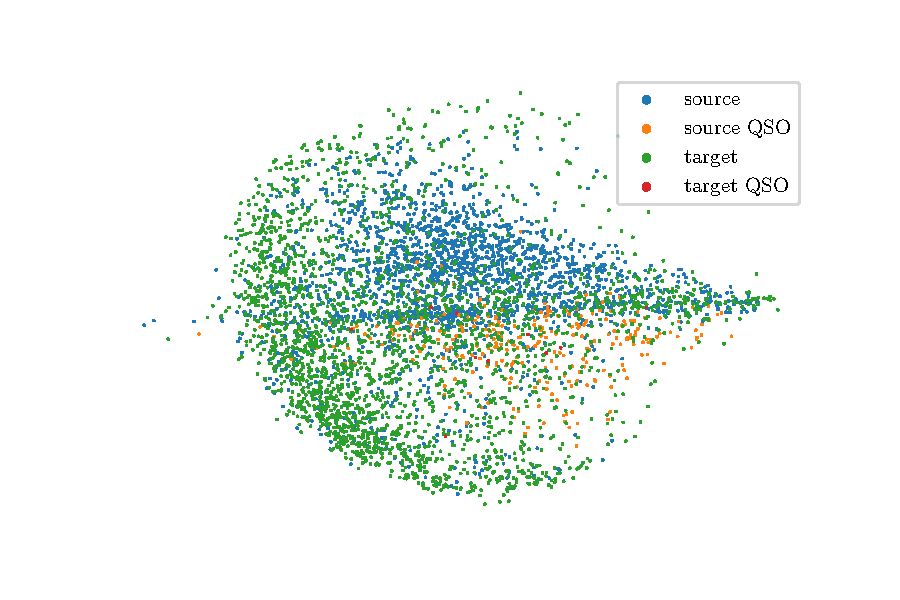
\includegraphics[width=\textwidth]{img/pca.pdf}
\caption[PCA visualisation of source and target data distributions]{
	The first two principal component of 2\,500 source
	and 2\,500 target data points.
	The projection shows that source data concentrate more in the middle
	whlie the target data seem to cluster on the edges.
	}
\label{pca}
\end{figure}

\textit{t-Distributed Stochastic Neighbor Embedding} (t-SNE)~\cite{maaten2008, wattenberg2016} is a popular method for visualisation of high-dimensional data.
The t-SNE method is non-linear, iterative
and performs different transformations of different regions.
A tunable hyperparameter of t-SNE is \textit{perplexity}
which is a guess about the number of neighbours of a data point.
Typically, the optimal value is between 5 and 50.

We reduce dimensionality with t-SNE for perplexities from \(\{5, 10, 30, 50, 100\}\).
The best result was for the value 30,
and the result is shown in Figure~\ref{tsne}.
The t-SNE embedding has a similar structure to Figure~\ref{pca} of PCA.
There are mostly source data in the centre and target data around it.
However, the separation between the centre and edges seems to be larger.
Still, there is the line component extending to the right.

t-SNE is often used in the papers presenting a deep domain adaptation methods
to show how feature extracted from a higher layer in an adapted network
are better mix when a domain adaptation method is employed.
On the other hand, when a network is not adapted the source and target data
can be easily visually separated in a t-SNE visualisation.

\begin{figure}
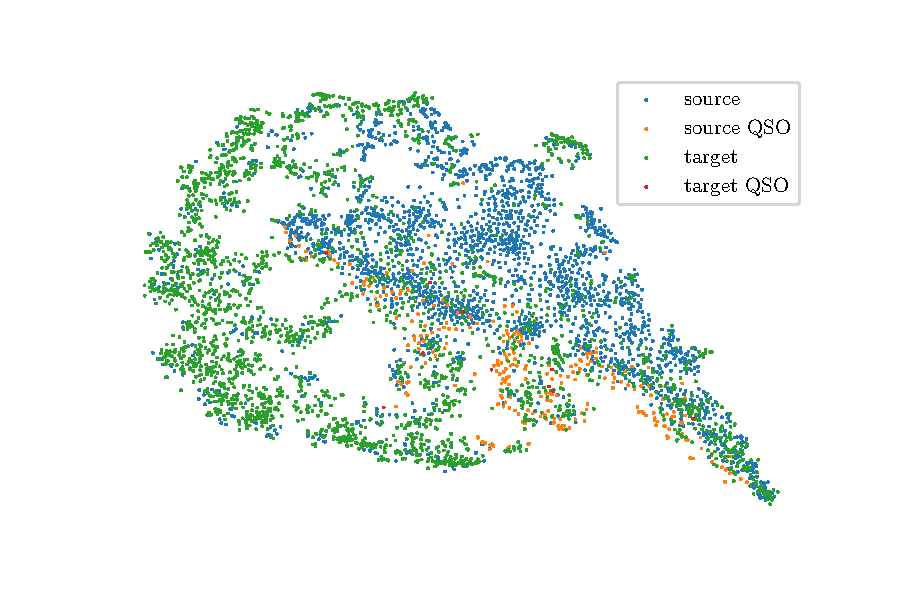
\includegraphics[width=\textwidth]{img/tsne.pdf}
\caption[t-SNE visualisation of source and target data distributions]{
	Embedding of t-SNE of the same data
	as in the reduction with PCA shows very similar result as PCA.
	However, there is more notable central sort of line component
	extending to the rigth.
	}
\label{tsne}
\end{figure}

\textit{Uniform Manifold Approximation and Projection} (UMAP)~\cite{mcinnes2018}
is a non-linear dimensionality reduction algorithm based on manifold learning and ideas from topological data analysis.
It achieves visualisations similar to t-SNE, but it is significantly faster.
Visualisation with UMAP is displayed in Figure~\ref{umap}
and has a very similar structure to t-SNE embedding in Figure~\ref{tsne}.

\begin{figure}
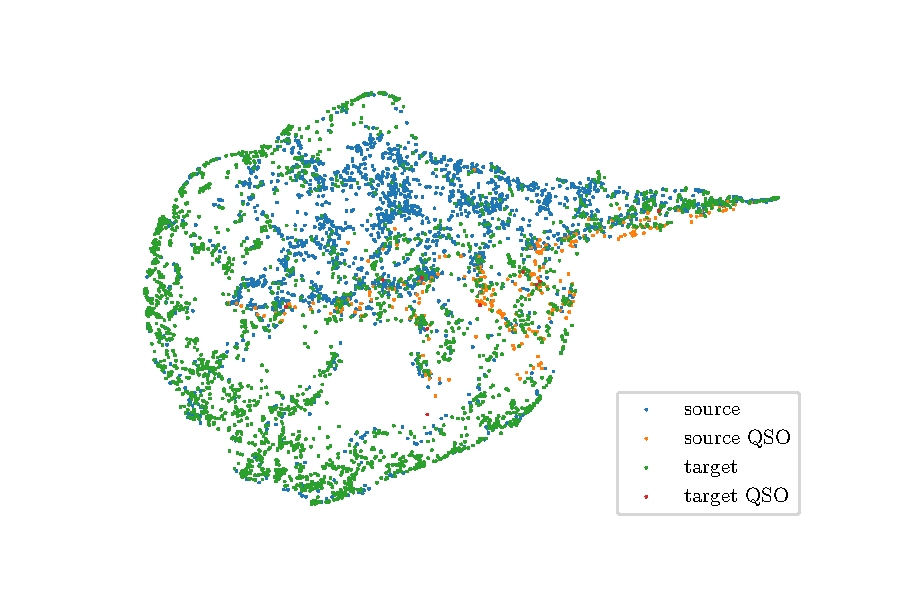
\includegraphics[width=\textwidth]{img/umap.pdf}
\caption[UMAP visualisation of source and target data distributions]{
	UMAP projection to two-dimensions confirm the previous visualisation
	with PCA and t-SNE.
	The source data tend to concentrate in the midlle
	while the target data are mostly out of center
	and there is the line component extending away from the center.
	}
\label{umap}
\end{figure}

\section{Baseline: Results without Deep Domain Adaptation}
\label{baseline}

Now, we are ready for training of neural networks
but before we will dive into deep domain adaptation
we will train a classical convulutional network
which will serve as baseline to
which we can compare results of networks augumented with deep domain adaptation.

As the baseline, we choose LeNet-5~\cite{lecun1998} convolutional neural network
which was originaly used to recognize hand written digits
of the MNIST dataset~\cite{lecun1998}.
We have choosen the architecture of LeNet-5
because it is the simplest model used in the DANN paper~\cite{ganin2016}.
However, the network is design for processing of two-dimensional images
while spectrum is a one-dimensional image.
Therefore, we have to substitude the two-dimensional convolutions with one-dimensional convolutions.
Moreover, we increased the kernel size and stride of pooling layer from 2 to 16
so that the output of the convolutional layer is reasonably big.
If we left the original pooling layer
the input to the first fully connected layer would be of size 43\,872.
in comparison the original input size 768 for the MNIST dataset.
The kernel size and stride of 16 will reduce the input size of our network to 672.
Figure~\ref{lenet_5} displays the final architecture
which we implemented in PyTorch~\cite{paszke2019}.

\tikzstyle{layer} = [align=center,draw=black,font=\tiny,rectangle,text centered]
\begin{figure}
\begin{center}
\subfloat[][LeNet-5]{
\begin{tikzpicture}[node distance=1.5cm]
	\node (conv1) [layer] {conv1\\5-32\\ReLU};
	\node (pool1) [layer,right of=conv1] {pool1\\16-16};
	\node (conv2) [layer,right of=pool1] {conv2\\5-48\\ReLU};
	\node (pool2) [layer,right of=conv2] {pool2\\16-16};
	\node (fc1) [layer,right of=pool2] {fc1\\100\\ReLU};
	\node (fc2) [layer,right of=fc1] {fc2\\100\\ReLU};
	\node (fc3) [layer,right of=fc2] {fc3\\1\\sigmoid};
	\draw [->] (conv1) -- (pool1);
	\draw [->] (pool1) -- (conv2);
	\draw [->] (conv2) -- (pool2);
	\draw [->] (pool2) -- (fc1);
	\draw [->] (fc1) -- (fc2);
	\draw [->] (fc2) -- (fc3);
\end{tikzpicture}
\label{lenet_5}
}\\
\subfloat[][DDC]{
\begin{tikzpicture}[node distance=1.5cm]
	\node (conv1) [layer] {conv1\\5-32\\ReLU};
	\node (pool1) [layer,right of=conv1] {pool1\\16-16};
	\node (conv2) [layer,right of=pool1] {conv2\\5-48\\ReLU};
	\node (pool2) [layer,right of=conv2] {pool2\\16-16};
	\node (fc1) [layer,right of=pool2] {fc1\\100\\ReLU};
	\node (bottleneck) [layer,right of=fc1,fill=red!50] {bottleneck\\64\\ReLU};
	\node (fc2) [layer,right of=bottleneck] {fc2\\100\\ReLU};
	\node (fc3) [layer,right of=fc2] {fc3\\1\\sigmoid};
	\draw [->] (conv1) -- (pool1);
	\draw [->] (pool1) -- (conv2);
	\draw [->] (conv2) -- (pool2);
	\draw [->] (pool2) -- (fc1);
	\draw [->] (fc1) -- (bottleneck);
	\draw [->] (bottleneck) -- (fc2);
	\draw [->] (fc2) -- (fc3);
\end{tikzpicture}
\label{ddc_architecture}
}\\
\subfloat[][DANN]{
\begin{tikzpicture}[node distance=1.5cm]
	\node (conv1) [layer] {conv1\\5-32\\ReLU};
	\node (pool1) [layer,right of=conv1] {pool1\\16-16};
	\node (conv2) [layer,right of=pool1] {conv2\\5-48\\ReLU};
	\node (pool2) [layer,right of=conv2] {pool2\\16-16};
	\node (fc1) [layer,right of=pool2,fill=blue!50] {fc1\\100\\ReLU};
	\node (fc2) [layer,right of=fc1,fill=blue!50] {fc2\\100\\ReLU};
	\node (fc3) [layer,right of=fc2,fill=blue!50] {fc3\\1\\sigmoid};
	\node (grl) [layer,below of=pool2,fill=green!50] {gradient\\reversar\\layer};
	\node (fc4) [layer,right of=grl,fill=green!50] {fc4\\100\\ReLU};
	\node (fc5) [layer,right of=fc4,fill=green!50] {fc5\\1\\sigmoid};
	\draw [->] (conv1) -- (pool1);
	\draw [->] (pool1) -- (conv2);
	\draw [->] (conv2) -- (pool2);
	\draw [->] (pool2) -- (fc1);
	\draw [->] (fc1) -- (fc2);
	\draw [->] (fc2) -- (fc3);
	\draw [->] (pool2) -- (grl);
	\draw [->] (grl) -- (fc4);
	\draw [->] (fc4) -- (fc5);
\end{tikzpicture}
\label{dann_architecture}
}\\
\subfloat[][DRCN]{
\begin{tikzpicture}[node distance=1.5cm]
	% encoder
	\node (conv1) [layer] {conv1\\5-32\\ReLU};
	\node (pool1) [layer,right of=conv1] {pool1\\16-16};
	\node (conv2) [layer,right of=pool1] {conv2\\5-48\\ReLU};
	% feature labelling
	\node (pool2) [layer,right of=conv2,fill=blue!50] {pool2\\16-16};
	\node (fc1) [layer,right of=pool2,fill=blue!50] {fc1\\100\\ReLU};
	\node (fc2) [layer,right of=fc1,fill=blue!50] {fc2\\100\\ReLU};
	\node (fc3) [layer,right of=fc2,fill=blue!50] {fc3\\1\\sigmoid};
	% decoder
	\node (conv3) [layer,below of=conv2,fill=green!50] {conv3\\5-48\\ReLU};
	\node (upsample1) [layer,left of=conv3,fill=green!50] {upsample1\\3659};
	\node (conv4) [layer,left of=upsample1,fill=green!50] {conv4\\5-32\\None};
	% connections
	\draw [->] (conv1) -- (pool1);
	\draw [->] (pool1) -- (conv2);
	\draw [->] (conv2) -- (pool2);
	\draw [->] (pool2) -- (fc1);
	\draw [->] (fc1) -- (fc2);
	\draw [->] (fc2) -- (fc3);
	\draw [->] (conv2) -- (conv3);
	\draw [->] (conv3) -- (upsample1);
	\draw [->] (upsample1) -- (conv4);
\end{tikzpicture}
\label{drcn_architecture}
}
\end{center}
\caption[Architectures of deep domain adaptation model from experiments]{
	Diagrams of all architectures used in our experiments.
	Note that the architectures are designed in such way
	that the classificator is the same for all models
	(minor exception is the adaptation layer in DDC).
	}
\end{figure}

Furthermore, Donahue et al. showed in the DeCAF (\textit{Deep Convolutional Activation Feature}) paper~\cite{donahue2014}
that features extracted from deep CNN can be repurposed to novel tasks
if the network were trained on a large fixed set in fully supervised fashion.
Meaning that it can be used for domain adaptation on its own.
Therefore, we can expected that our CNN trained on the large SDSS
will be able to find features beneficial for domain adaptation.
Still the DeCAF paper showed that
deep CNN cannnot remove domain bias completelly.
Therefore, there is a space for improvement with deep domain adaptation
and DDC, Deep CORAL and DANN build in experiment on result of DeCAF
because they use AlexNet~\cite{krizhevsky2012} pre-trained on ImageNet dataset.

We trained our adapted LeNet-5 on batches of size 64 for 20 epochs
with the Adam optimiser~\cite{kingma2014} in its default setting
and used the \textit{binary cross entropy loss} defined as:

\begin{equation}
	\mathit{BCE}(\theta) = -\frac{1}{M} \sum_i^M [y_i \log \hat{y}_i + (1 - y_i) \log(1 - \hat{y}_i)],
\end{equation}

where \(\theta\) are all parameters of a model,
\(M\) is the batch size,
\(y_i \in \{0, 1\}\) is the true label
and \(\hat{y}_i \in [0, 1]\) are the model predictions of the \(i\)-th example in the batch.
Furthermore, we intialised the weights and biases in accordance with Xavier initialisation~\cite{glorot2010}.
That is weights of our neural network are sampled from uniform distribution \(\mathcal{U}\):

\begin{equation}
	\mathcal{U}\left(
	-\frac{\sqrt{6}}{\sqrt{\mathit{in} + \mathit{out}}},
	\frac{\sqrt{6}}{\sqrt{\mathit{in} + \mathit{out}}}
	\right),
\end{equation}

where \(\mathit{in}\) is the number of input units of a layer
and \(\mathit{out}\) is the number of output units
and biases are set to zero.

% TODO describe training progress

\begin{figure}
\subfloat[][Losses]{
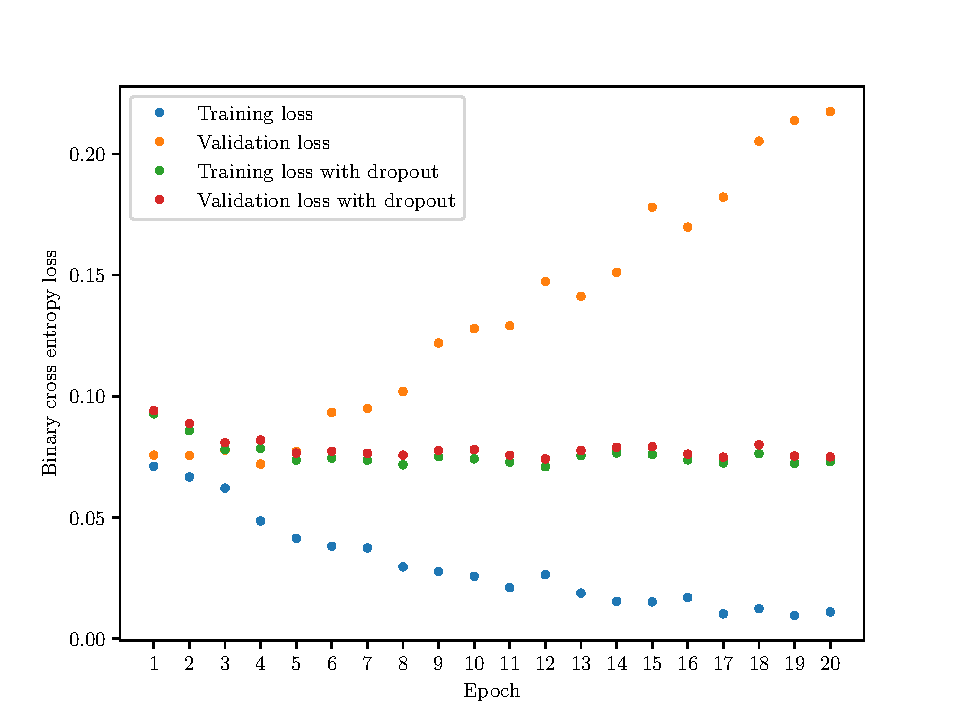
\includegraphics[width=.5\textwidth]{img/lenet_losses.pdf}
}
\subfloat[][\(F_1\) score]{
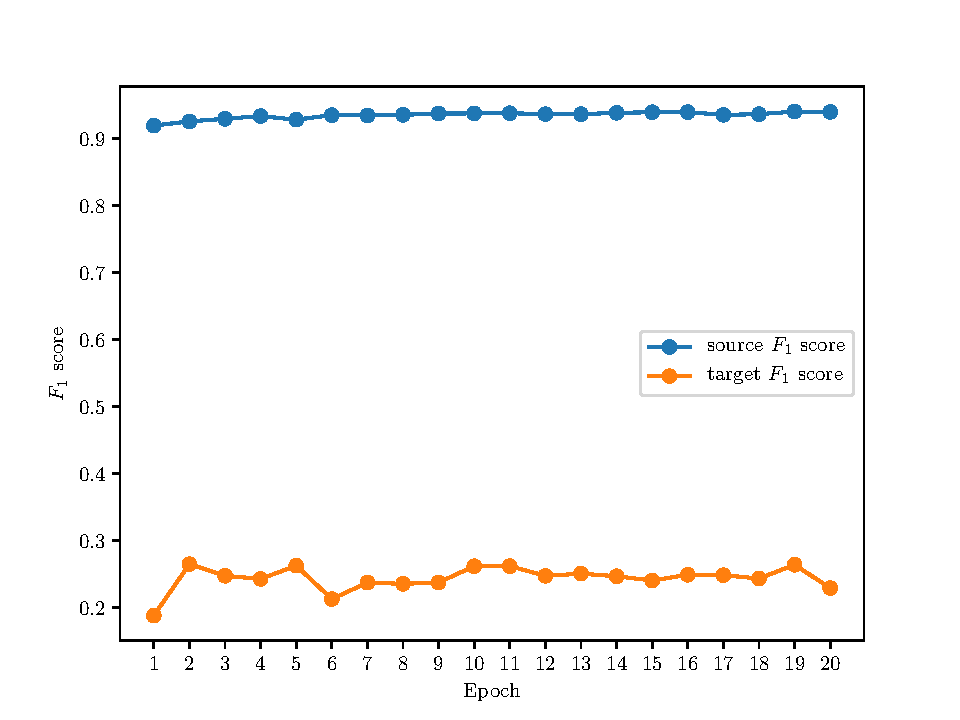
\includegraphics[width=.5\textwidth]{img/lenet_f1.pdf}
}
\caption{Training of LeNet-5}
\label{lenet_losses}
\end{figure}

\textit{Recall} \(r\), \textit{precision} \(p\)
and \textit{\(F_1\) score} is the harmonic mean between \textit{precision} and \textit{recall}:

\begin{align}
	r &= \frac{\mathit{TP}}{(\mathit{TP} + \mathit{FN})}, \\
	p &= \frac{\mathit{TP}}{(\mathit{TP} + \mathit{FP})}, \\
	F_1 &= \frac{2}{r^{-1} + p^{-1}} = 2 \frac{r p}{r + p},
\end{align}

where \(r\) is recall, \(p\) is precision,
\(\mathit{TP}\) is the number of correctly classified QSOs,
\(\mathit{FN}\) is the number of QSOs incorrectly classified as non-QSOs
and \(\mathit{FP}\) is the number of non-QSOs classified as QSOs.
When precision and recall are perfect
\(F_1\) score reaches its best value one and at worst can be zero.

The result of our baseline are quite good on the source domain.
Note that all metrics were computed on either the source or target validation sets in all our experiments.
The source \(F_1\) score is 0.9397.
The source recall is 95,82\% and the source precision is 92,19\%.
That are quite high number on the source domain.
However, the target \(F_1\) score is 0.2294 (target precision is is 13.48\% and target recall 76.84\%).
That is a very poor result for the target data.
We see that there probably is a huge domain discrepancy.
Therefore, a pontentialy huge space for domain adaptation methods.

\begin{table}
\begin{center}
\subfloat[][Source confusion matrix]{
\begin{tabular}{|l|r|r|}
	\hline
	Predicted class & \multicolumn{2}{c|}{Actual class} \\ \hline \hline
	& QSO & non-QSO \\ \hline
	QSO & 6\,278 & 532 \\ \hline
	non-QSO & 274 & 42\,916 \\ \hline
\end{tabular}
}
\subfloat[][Target confusion matrix]{
\begin{tabular}{|l|r|r|}
	\hline
	Predicted class & \multicolumn{2}{c|}{Actual class} \\ \hline \hline
	& QSO & non-QSO \\ \hline
	QSO & 146 & 937 \\ \hline
	non-QSO & 44 & 48\,873 \\ \hline
\end{tabular}
}
\end{center}
\end{table}

\section{Experiments with Deep Domain Adaptation}

We set the baseline result with classical CNN.
Now, we apply four deep domain adaptation method to the same data
to show if astronomical spectroscopy can benefit from domain adaptation
based on neural networks.

We start with two discrepancy-based approach which are DDC and Deep.
Then, we continue will DANN
which is an adversarial-based domain adaptation method
and we with reconstruction based DRCN.
We conclude with evaluation and comparison of results.

\subsection{DDC: Deep Domain Confusion}

Firts deep domain adaptation method is \textit{Deep Domain Confusion} (DDC).
DDC reduces the domain discrepancy (maximises domain confusion)
by extending classification loss of a neural network with the MMD loss
(see Equation~\ref{ddc_loss}).
The MMD loss is enforced on \textit{adaptation layer}
that serves information bottleneck for domain confusion.
More details on DDC are in Subsection~\ref{discrepancy_da}.

To select the size and placement of the adaptation layer,
we followed the same procedure as in the DDC paper~\cite{tzeng2014}.
Firstly, we took the LeNet-5 trained in previous Section~\ref{baseline}
and extracted features from the first and second fully-connected layer
(the last fully-connected layer has a trivial width)
for all validation examples.
Then, we computed MMD between the source and target data at each layer with the extracted features.
The intuition is to place the adaptation layer after a layer with smallest MMD
because low MMD means more domain invariant features.
We measured that the MMD at the first fully-connected layer is 50.70
while MMD at the second fully-connected layer is 53.33.
Therefore, we will place the adaptation layer after the first fully-connected layer.
Secondly, we have to optimise the width of the adaptataion layer.
Therefore, we trained the LeNet with the adaptation layer of sizes
from \(\{4, 8, 16, 32, 64\}\) excluding the low width of 2
and not exceeding the output size of previous layer.
The stepping is power of two as in the original paper.
Figure~\ref{adaptation_layer} plots the resulting MMD values for different setting
and shows that the width 64 is the best.

The final architecture of our DDC network is in Figure~\ref{ddc_architecture}.
It is the baseline CNN with the adaptation layer of width 64
after the first fully-connected layer.

\begin{figure}
	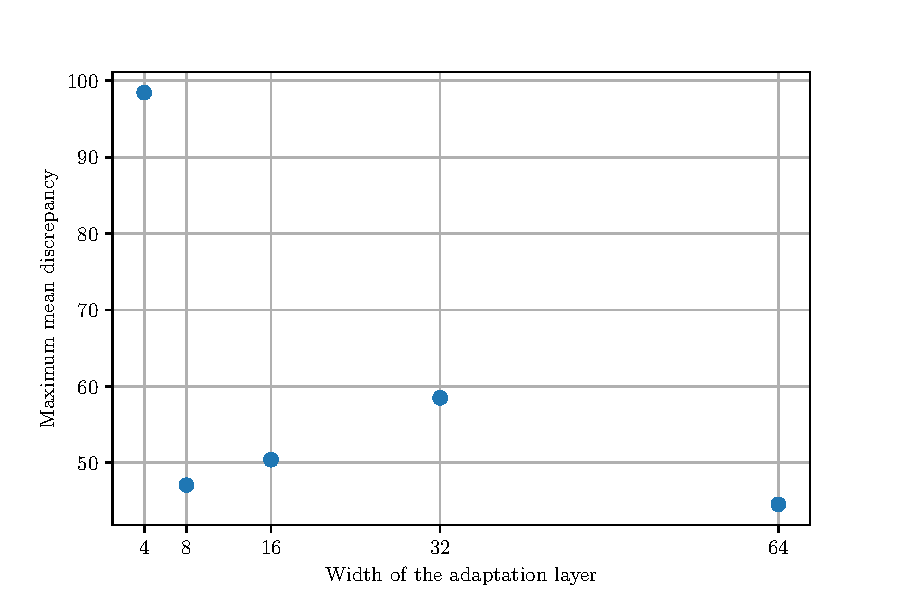
\includegraphics[width=\textwidth]{img/adaptation_layer_width.pdf}
	\caption{Width of the adatpation layer}
	\label{adaptation_layer}
\end{figure}

Furthermore, we set the trade-off parameter \(\lambda\)
between the binary cross entropy loss
and the MMD loss to 0.25 as in the DDC experiments
and trained the network in the same way as described in previous section~\ref{baseline}
(Xavier initialisation, Adam optimizer, batch size 64 and 20 epochs).

Figure~\ref{ddc_training} displays training progress of DDC
which is correctly learning to classify.
Moreover, we see that MMD is also minimalised in the bottom plot of Figure~\ref{ddc_mmds}
while if we train the network without enforcing MMD loss (\(\lambda = 0\))
then the MMD is growing as in the top plot of Figure~\ref{ddc_mmds}.

\begin{figure}
\subfloat[][Losses]{
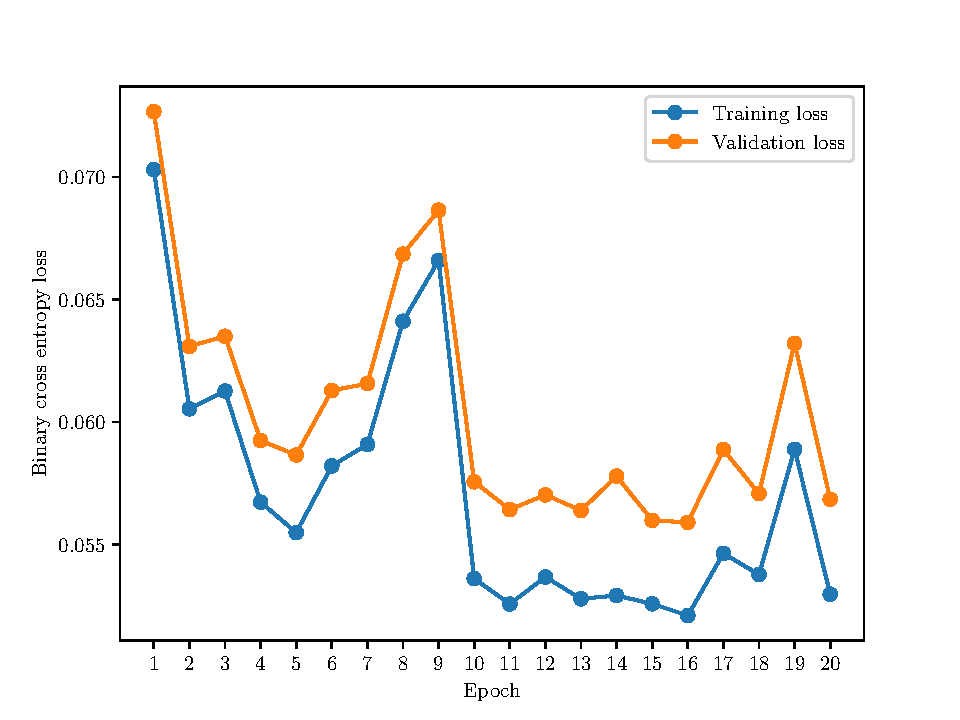
\includegraphics[width=.5\textwidth]{img/ddc_losses.pdf}
}
\subfloat[][Maximum mean discrepancy]{
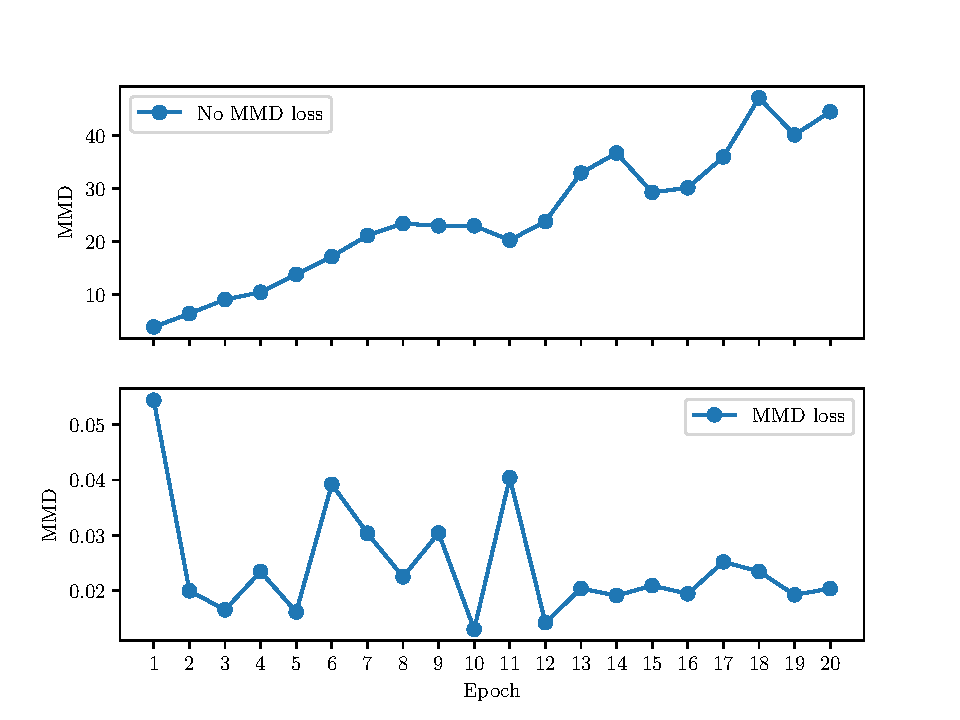
\includegraphics[width=.5\textwidth]{img/ddc_mmds.pdf}
\label{ddc_mmds}
}
\caption{Training of DDC}
\label{ddc_training}
\end{figure}

Although, training run as expected
DDC achived poor result in comparison to baseline.
The \(F_1\) score on source data is 0.9354 and on target 0.2005
that is lower than the baseline in both cases.
Precision on target is 11.51\% and
the only imporovement is recall of value 77.89\%
but that is probably caused by the decrease in precision.
Table~\ref{ddc_confusion} shows a confusion matrix of the result.

\begin{table}
\begin{center}
\begin{tabular}{|l|r|r|}
	\hline
	Predicted class & \multicolumn{2}{c|}{Actual class} \\
	\hline \hline
	& QSO & non-QSO \\ \hline
	QSO & 148 & 1\,138 \\ \hline
	non-QSO & 42 & 48\,672 \\ \hline
\end{tabular}
\end{center}
\caption{Target confusion matrix}
\label{ddc_confusion}
\end{table}

\subsection{Deep CORAL: Deep Correlation Alignment}

\textit{Deep Correlation Alignment} (Deep CORAL) is very similar to DDC.
While DDC aligns means of source and target distributions with MMD loss
Deep CORAL aligns correlations with CORAL loss
(see Equations~\ref{coral_loss} and \ref{deep_coral_loss}).
Moreover, Deep CORAL applies the CORAL loss straight to a layer in a network
not creating an adaptation layer.
We implemented Deep CORAL with inspiration from original
code\footnote{Available from: \url{https://github.com/visionlearninggroup/CORAL}}
and follow all the step described in corresponding paper~\cite{sun2016}.

Originally, the architecture underlying Deep CORAL is AlexNet~\cite{krizhevsky2012}.
There the CORAL loss was put on the last layer that has ten output units.
However, our neural network has to have one output unit
so applying CORAL loss does not make sense.
Therefore, we applied the CORAL loss to the second fully-connected layer
of our LeNet-5 architecture in Figure~\ref{lenet_5}.
Then, we optimised the trade-off between classification and CORAL loss
\(\lambda\) from \(\{0.5, 0.1, 0.05, 0.01, 0.005, 0.001, 0.0005, 0.0001\}\).
The best is \(\lambda = 0.0005\) which makes the calssification loss
and the CORAL loss of similar magnitude as suggested by the paper
(see Figure~\ref{deep_coral_losses}).
Furthermore, we used the same batch size of value 128
as in original experiments of Deep CORAL.
The architecture is intialised in the same way as baseline
and optimised with Adam for 20 epochs.

Firstly, we trained our Deep CORAL with \(\lambda = 0\) to see
how the correlation alignment grows.
Figure~\ref{deep_coral_coral} shows the same behavior of correlation alignment
without enforcing the minimisation of correlation loss as in the original paper.
Then, we carried out experiment with the best \(\lambda = 0.0005\)
and obtained the training progress in Figure~\ref{deep_coral_losses}.
However, the result are unsatisfactory as in the case of DDC.

\begin{figure}
\subfloat[][Training of Deep CORAL]{
	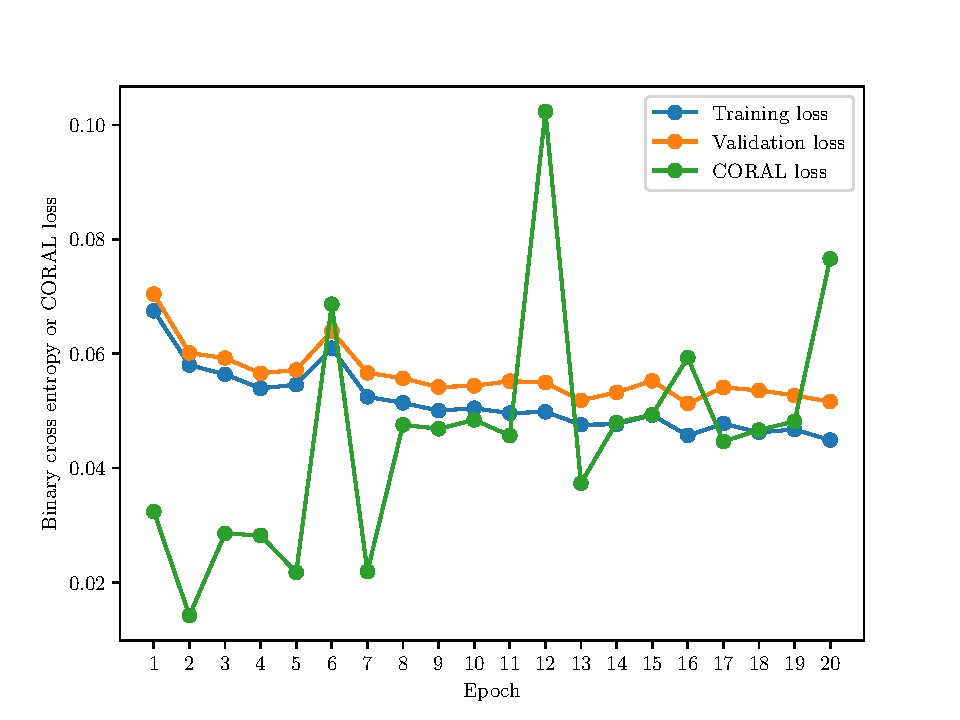
\includegraphics[width=.5\textwidth]{img/deep-coral_losses.pdf}
	\label{deep_coral_losses}
}
\subfloat[][CORAL with using CORAL loss]{
	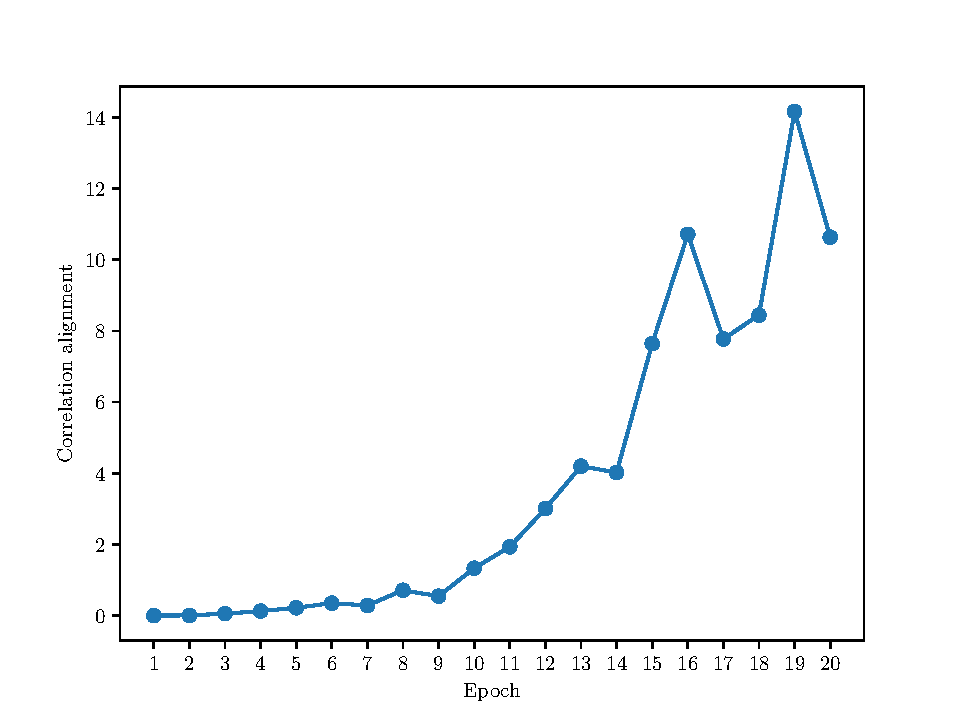
\includegraphics[width=.5\textwidth]{img/deep-coral_coral.pdf}
	\label{deep_coral_coral}
}
\caption{Losses of Deep CORAL}
\label{deep_coral_training}
\end{figure}

Source data \(F_1\) score is of value 0.9396
that is almost the same as baseline
and there is also a small but insignificant imporovement in the target \(F_1\) score
which is of value 0.2509.
Target precision is 14.97\% and target recall is 77.37\%.
These values are gains but their are too small
and the model with such small precision is useless for identification of QSOs.

\begin{table}
\begin{center}
\begin{tabular}{|l|r|r|}
	\hline
	Predicted class & \multicolumn{2}{c|}{Actual class} \\
	\hline \hline
	& QSO & non-QSO \\ \hline
	QSO & 147 & 835 \\ \hline
	non-QSO & 43 & 48\,975 \\ \hline
\end{tabular}
\end{center}
\caption{Target confusion matrix of Deep CORAL}
\end{table}

\subsection{DANN: Domain-Adversarial Neural Network}

\textit{Domain-Adversarial Neural Network} (DANN) is an adversarial-based domain adaptation method.
Our DANN architecture is depicted in Figure~\ref{dann_architecture}.
It consist of a feature extractor, a predictor and a domain classifier
that acts adversarially agains the feature extractor
enforcing domain invariant representation.
Further details are in Subsection~\ref{adversarial_da}.

We code and schedule hyperparameters of DANN accoring to original
implementation\footnote{Available from: \url{http://sites.skoltech.ru/compvision/projects/grl/}}
and two papers where DANN was published~\cite{ganin2015, ganin2016}.
The learning rate schedule for SGD with momentum:

\begin{equation}
	\mu_p = \frac{\mu_0}{(1 + \alpha p)^\beta},
\end{equation}

where \(p\) is the training progress linearly changign from 0 to 1 in every iteration,
initial learning rate \(\mu_0 = 0.01\), \(\alpha = 10\) and \(\beta = 0.75\).

The domain adaptation parameter \(\lambda\) from Equation~\ref{dann_loss}
start at 0 and grows to 1 with schedule:

\begin{equation}
	\lambda_p = \frac{2}{1 + e^{-\gamma p}} - 1,
\end{equation}

where \(p\) is again the training progress
and \(\gamma\) that was set to 10 in the original paper.

\begin{figure}
	\subfloat[][Training losses of DANN]{
		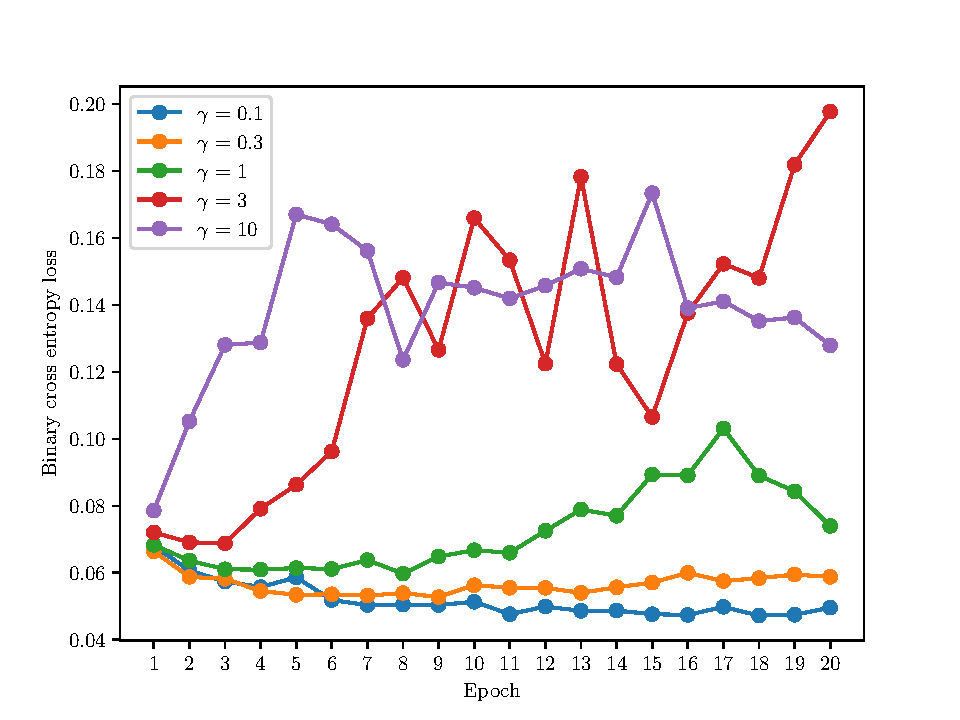
\includegraphics[width=.5\textwidth]{img/dann_losses.pdf}
	}
	\subfloat[][\(F_1\) score for different \(\gamma\)]{
		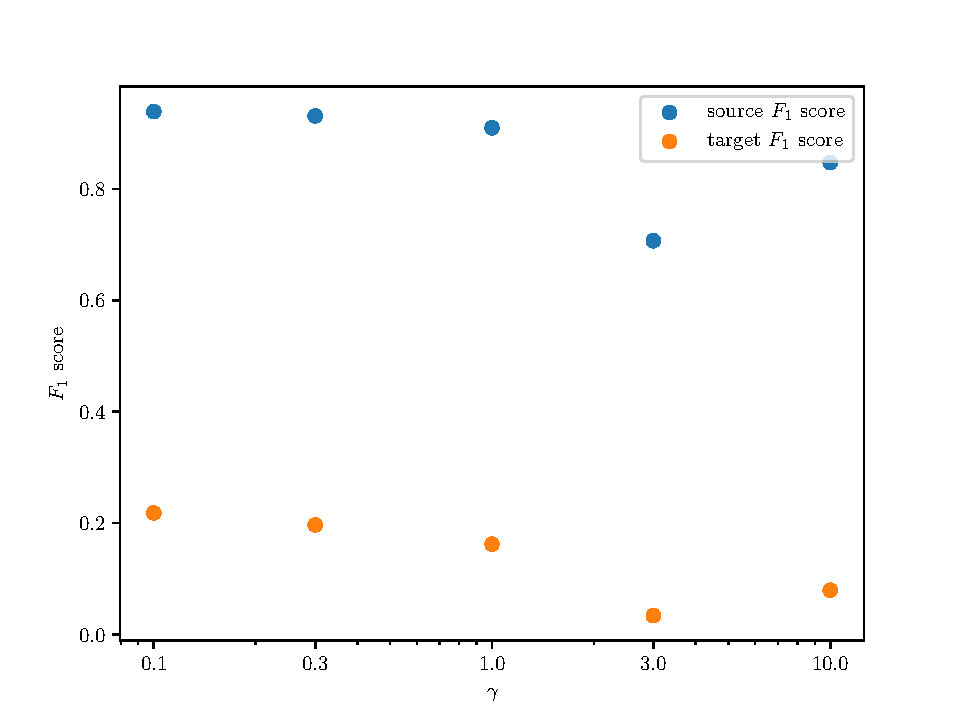
\includegraphics[width=.5\textwidth]{img/dann_f1.pdf}
	}
	\caption{Training of DANN}
	\label{dann_training}
\end{figure}

Note that binary cross entropy loss is used for both the classification and domain loss.
The optimiser is SGD with the learning rate schedule and momentum 0.9,
the network is initialised as our baseline model
and the batch size is 128 where first half are source domain data
and the second half are the target domain data.

Although following the original impelementation as closely as possible
and doing hyperparameter optimisation of \(\gamma \in \{0.1, 0.3, 1, 3, 10\}\)
we were not able to get reasonable results with DANN.
We infer from Figure~\ref{dann_training} that
if gamma is high the training will diverge.
On the other hand, if gamma is low \(F_1\) score regress.

\subsection{DRCN: Deep Reconstruction-Classification Network}

The last deep domain adaptation model is
\textit{Deep Reconstruction-Classification Network} (DRCN)
which uses reconstruction of target data as auxiliary task.
Intuition is that the auxiliary task
will enfore the network to capture also the structure of target data space.
More detail are provided in~Subsection~\ref{reconstruction_da}.

We followed the original implementation\footnote{Available from: \url{https://github.com/ghif/drcn}} of DRCN~\cite{ghifary2016}.
There is one big difference between the original paper and the official paper
that is the order of training loops.
The paper states that the network in an epoch
should firstly be trained for classification task
and then for reconstruction task.
The implementation work the other way around.

We followed the working implementation and train for reconstruction first.
Accordingly, we used Adam optimiser with batch size 128 for 20 epochs
and Xavier initialisation.
The trade-off parameter \(\lambda\) was set to 0.5.
Figure~\ref{drcn_training} shows the training progress
and Figure~\ref{reconstruction} show that the network is able to learn
good representation that can supress noise
while maitaining important spectral lines.

\begin{figure}
\subfloat[][Validation reconstruction loss of DRCN]{
	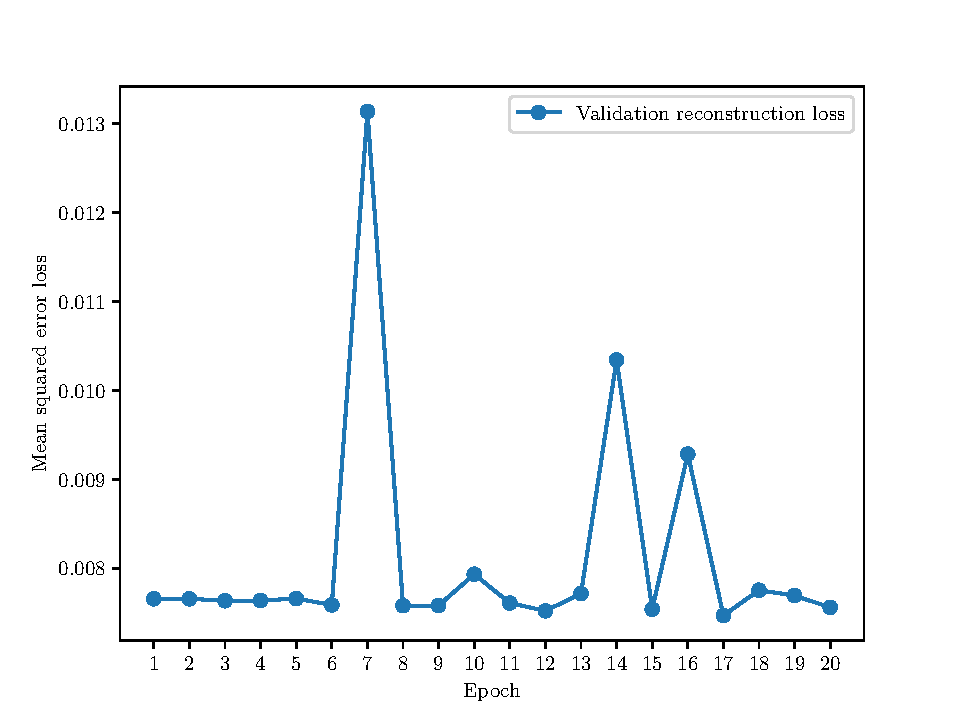
\includegraphics[width=.5\textwidth]{img/drcn_rec-loss.pdf}
}
\subfloat[][\(F_1\) score of DRCN and our LeNet-5]{
	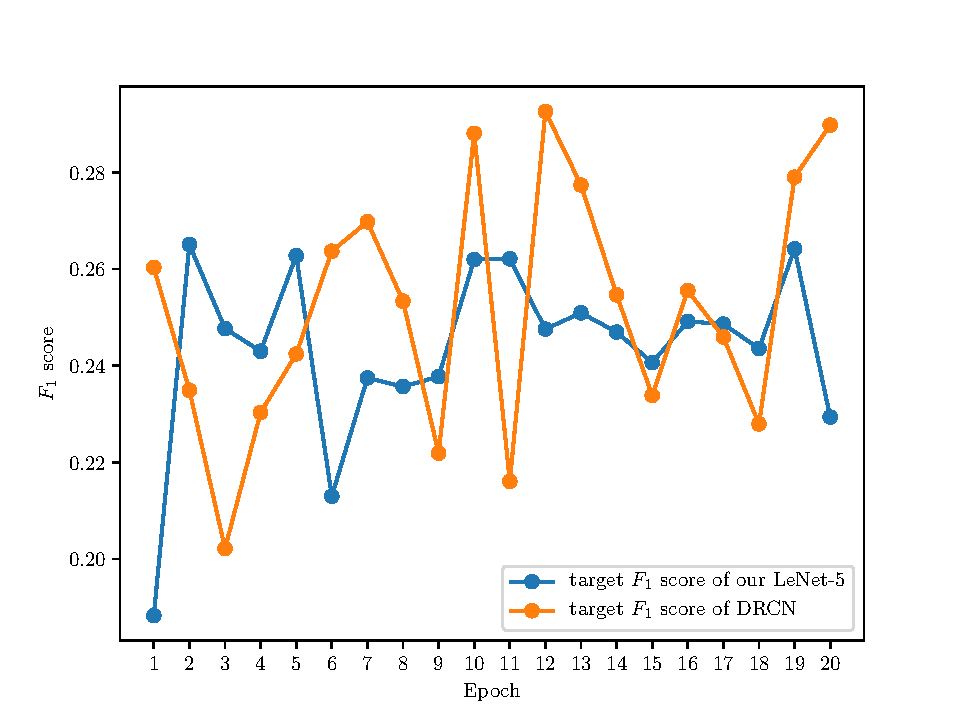
\includegraphics[width=.5\textwidth]{img/drcn_f1.pdf}
	\label{drcn_f1}
}
\caption{Training of DRCN}
\label{drcn_training}
\end{figure}

\begin{figure}
	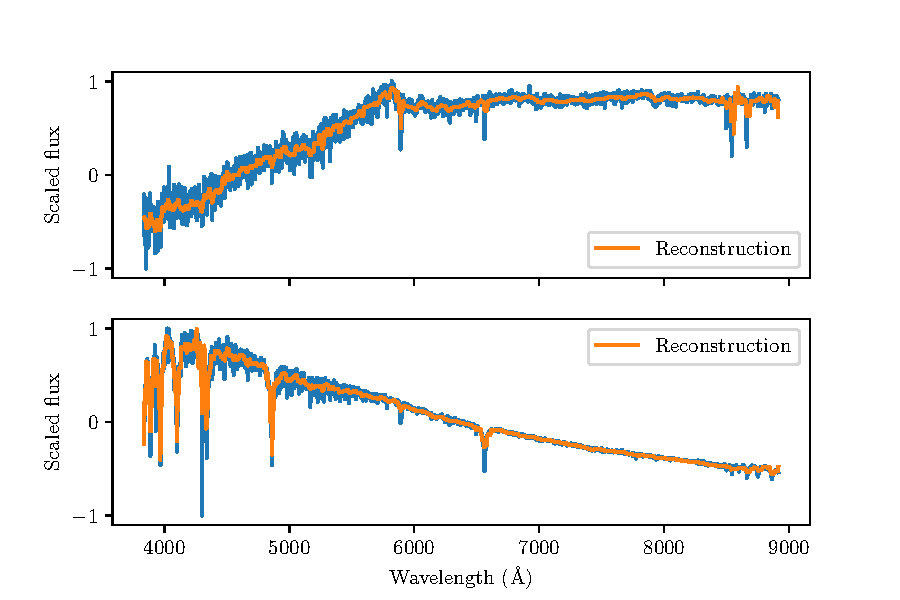
\includegraphics[width=\textwidth]{img/reconstructed_spectra.pdf}
	\caption{Spectra reconstructed with DRCN}
	\label{reconstruction}
\end{figure}

However, achiving poor results with previous methods
we did not suppose to get good result now.
Source \(F_1\) score is 0.9393 and target \(F_1\) score 0.2898
which is better than baseline
but the development of the \(F_1\) score in Figure~\ref{drcn_f1} suggest no significance.
Target precision is 17.97\% whcich si the best so far
but target recall 74.74\% is the worst.

\begin{table}
\begin{center}
\begin{tabular}{|l|r|r|}
	\hline
	Predicted class & \multicolumn{2}{c|}{Actual class} \\
	\hline \hline
	& QSO & non-QSO \\ \hline
	QSO & 142 & 648 \\ \hline
	non-QSO & 48 & 49\,162 \\ \hline
\end{tabular}
\end{center}
\caption{Target confusion matrix of DRCN}
\end{table}

\section{Discussion of Experiments}

We summarise the results of baseline and deep domain adaptation methods in Table~\ref{summary}.
We do not include the performance of DANN
because we were not able to train it correctly even though we did hyperparameter optimisation.
Table~\ref{summary} clearly shows that domain adaptation based on neural networks do cannot significantly improve performance in comparison to baseline
when applied to astronomical data.
We would expect an increase in a metric of at least 5\% as in the original paper of the deep domain methods on standard academical datasets.

\begin{table}
\begin{center}
\begin{tabular}{|l|r|r|r|r|}
	\hline
	Method & Source \(F_1\) & Target \(F_1\) & Precision (\%) & Recall (\%) \\
	\hline \hline
	Baseline & 0.9397 & 0.2294 & 13.48 & 76.84 \\ \hline
	DDC & 0.9354 & 0.2005 & 11.51 & 77.89 \\ \hline
	Deep CORAL & 0.9396 & 0.2509 & 14.97 & 77.37 \\ \hline
	DRCN & 0.9393 & 0.2898 & 17.97 & 74.74 \\ \hline
\end{tabular}
\end{center}
\caption{Summary table}
\label{summary}
\end{table}

Domain adaptation did not succeed,
although the distributions of the source and target domain are different.
We prove the difference in Subsection~\ref{comparison},
where we compare the two surveys.
Furthermore, we confirmed the discrepancy with dimensionality reduction techniques.
All three PCA, t-SNE and UMAP shows that the data does not occupy a single cluster,
but the SDSS spectra concentrate in the centre and LAMOST spectra on the edges
(see Figures~\ref{pca}, \ref{tsne} and \ref{umap}).

Also, the deep domain adaptation method behaved correctly.
DDC kept the MMD between the source and target distributions low,
as shown in~Figure~\ref{ddc_mmds}.
Deep CORAL achieved the same with the CORAL metric for distribution difference
(see Figure~\ref{deep_coral_training}),
and DRCN learnt the auxiliary reconstruction task
that is supposed to support domain adaptation
(see Figure~\ref{reconstruction}).
Moreover, even, hyperparameter optimisation cannot improve the performance of the deep domain adaptation methods.

All in all, we hypothesise the problem is in the data.
Therefore, we visualise the incorrect classification of the baseline
(the errors were almost the same for all the methods).
In Figure~\ref{src_fp} and Figure~\ref{src_fn}, we display source false positives and source false negatives, respectively.
At the same time, we display target false positives and target false negatives in Figure~\ref{trg_fp} and Figure~\ref{trg_fn}, respectively.
% TODO other examples are in the Appendix

We believe the misclassifications are evidence for our conclusion
that the problem is in our imperfect datasets.
The incorrectly classified examples are QSOs not yet identified by a catalogue of the surveys.
There are also spectra incorrectly classified as a QSO by the official catalogues.
Moreover, there are spectra with artefacts
(for example, missing measurements at paricular wavelengths, wrong extraction from CCD chip). 
However, the original deep domain adaptation methods are trained on well-prepared and clean data.
For example, all data in the MNIST~\cite{lecun1998} or USPS~\cite{hull1994} are well-defined digits,
and the same applies to the Office dataset~\cite{saenko2010} commonly used as a domain adaptation benchmark.
Such well-formed datasets provide a comfortable environment for basic research.
On the other side, they do not resemble the real world or scientific situation.
That is a big issue for the application of such method to scientific data.
As we have shown, astronomy provides such a volume of data that is impossible to make clean.
Therefore, we need either robust machine learning algorithms
or automatic procedures that clean data possibly also based on machine learning.
However, by cleaning the data, we might lose some interesting objects with strange physical properties.
Maybe, the imperfect data problem is the reason
why previous applications of domain adaptation in astronomy used active learning (a human expert)
after domain adaptation (see Section~\ref{da_astronomy}).

\begin{figure}
\subfloat[][\texttt{spec-0813-52354-0020}]{
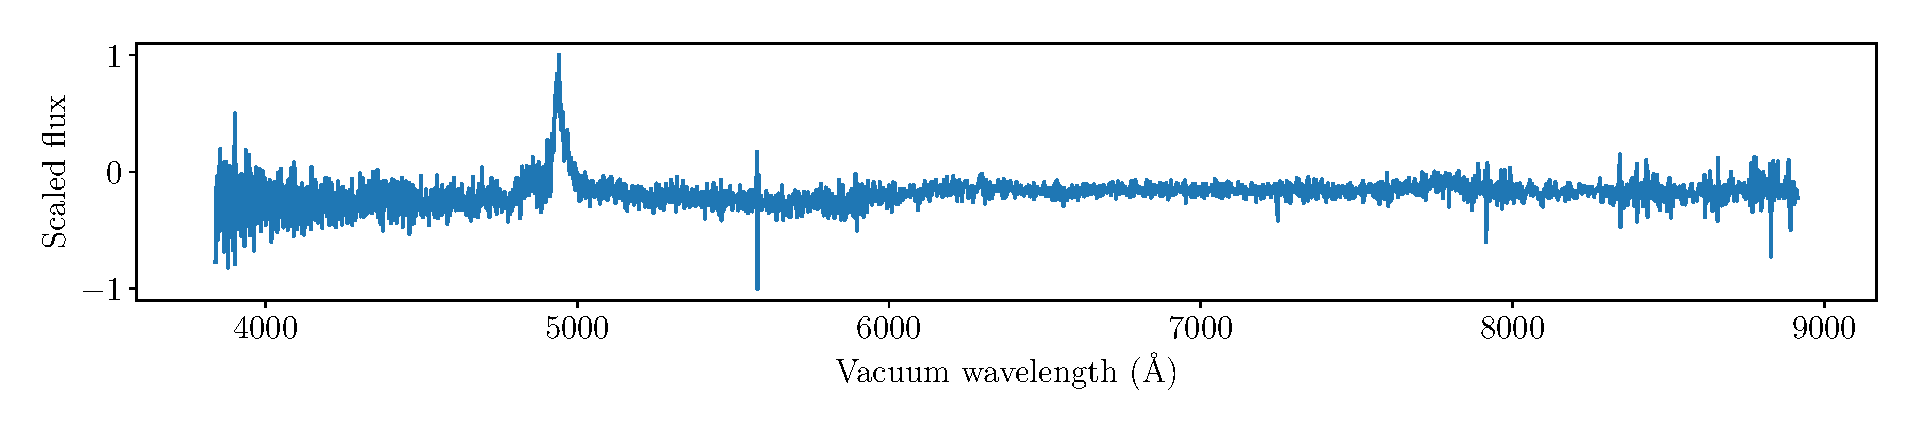
\includegraphics[width=\textwidth]{img/src_fn/spec-0813-52354-0020.pdf}
}\\
\subfloat[][\texttt{spec-0967-52636-0214}]{
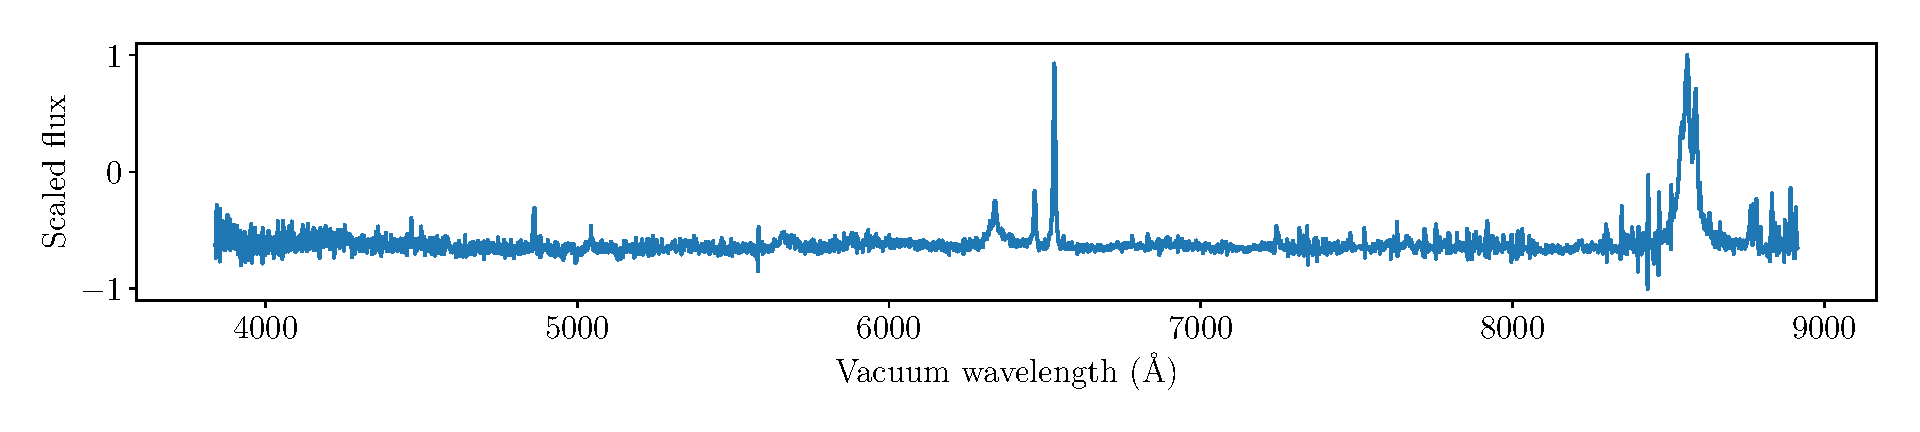
\includegraphics[width=\textwidth]{img/src_fn/spec-0967-52636-0214.pdf}
}\\
\subfloat[][\texttt{spec-1199-52703-0317}]{
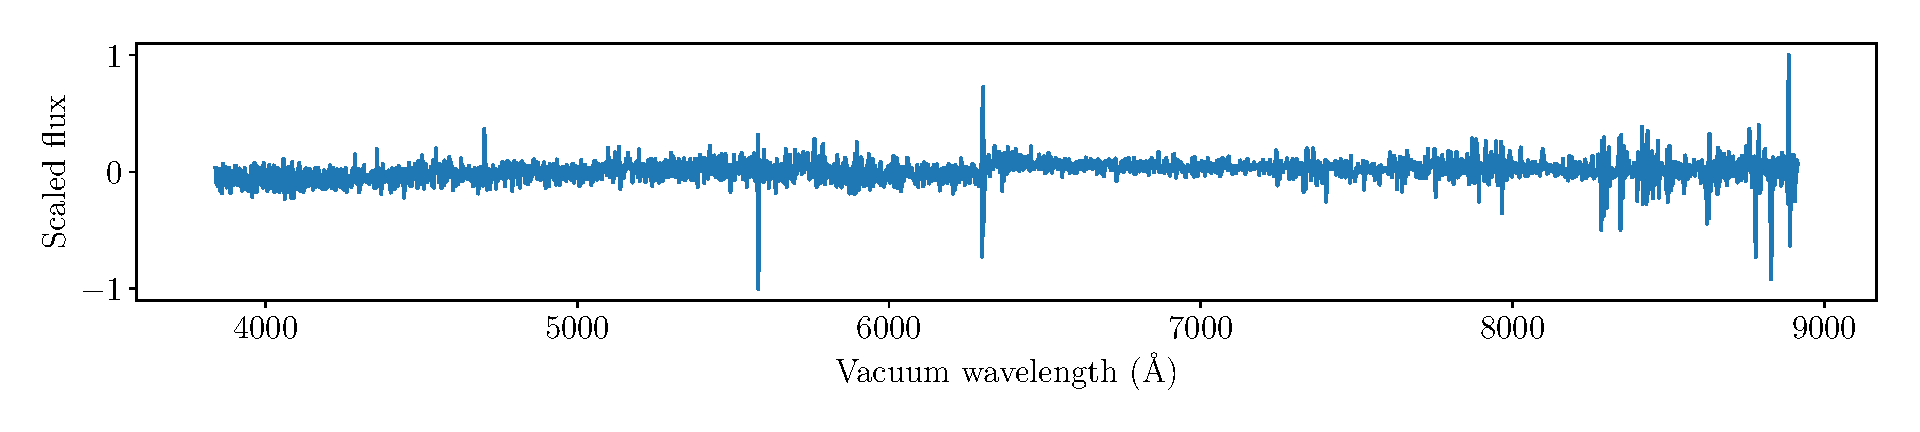
\includegraphics[width=\textwidth]{img/src_fn/spec-1199-52703-0317.pdf}
}\\
\subfloat[][\texttt{spec-1992-53466-0317}]{
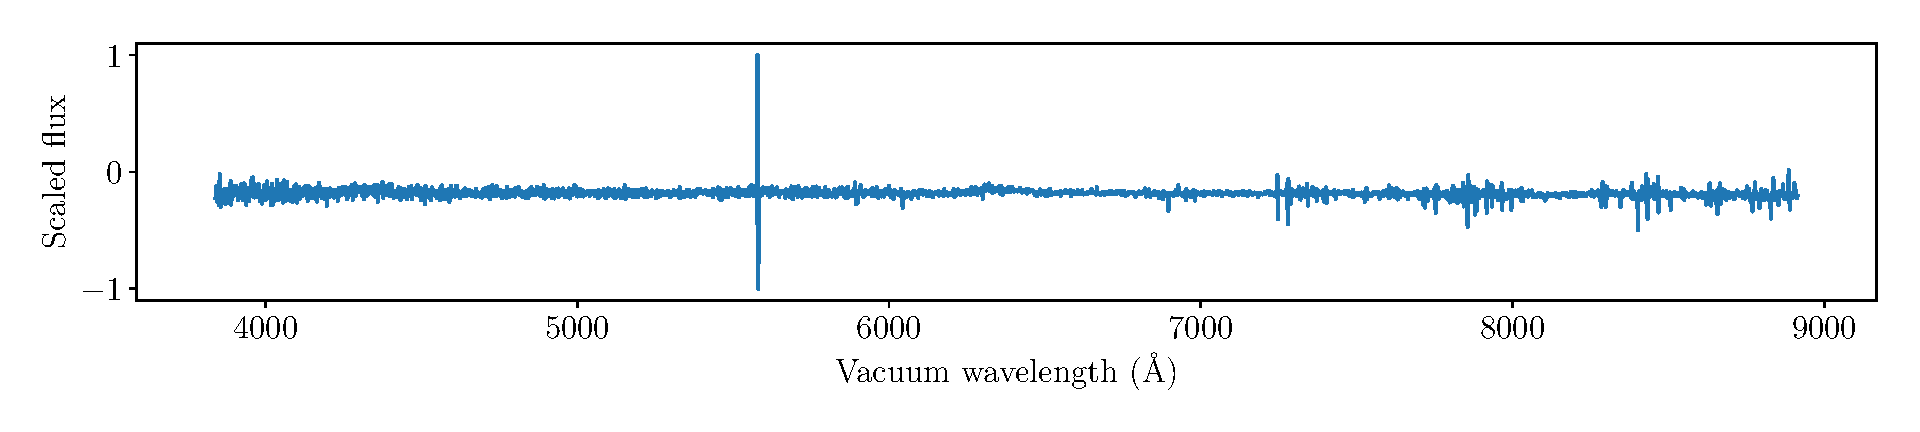
\includegraphics[width=\textwidth]{img/src_fn/spec-1992-53466-0317.pdf}
}\\
\subfloat[][\texttt{spec-2656-54484-0409}]{
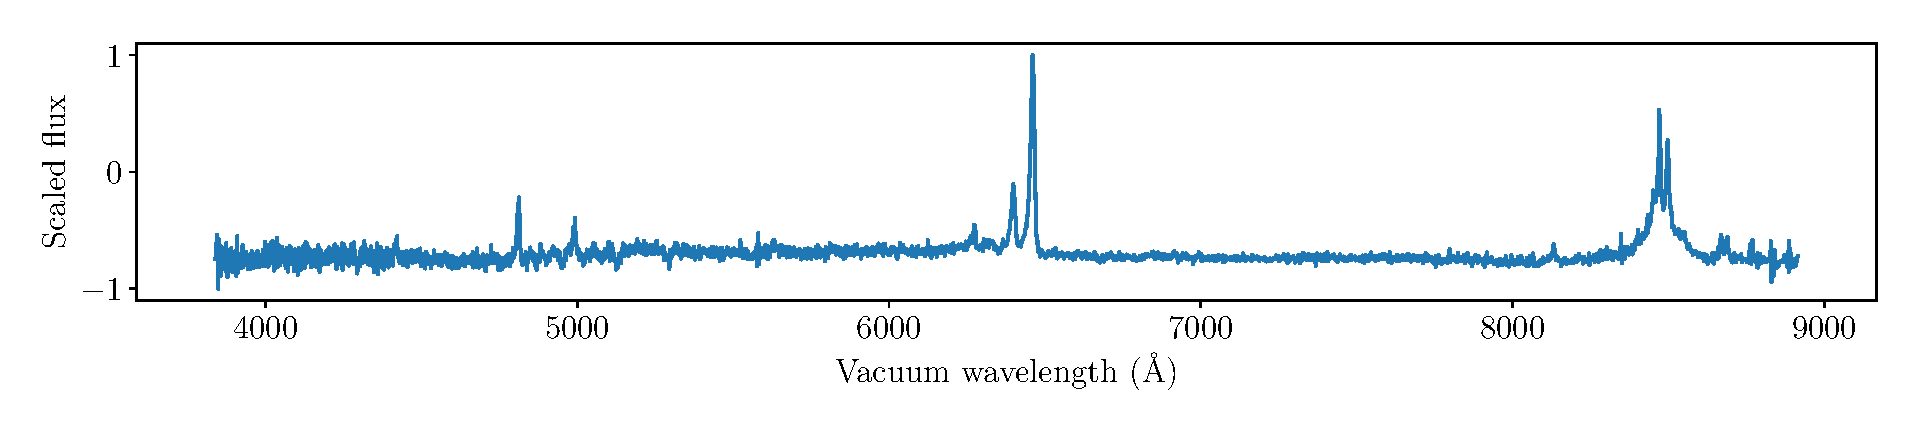
\includegraphics[width=\textwidth]{img/src_fn/spec-2656-54484-0409.pdf}
}
\caption{First sample of source false negatives}
\label{src_fn}
\end{figure}

\begin{figure}
\subfloat[][\texttt{spec-0406-51900-0598}]{
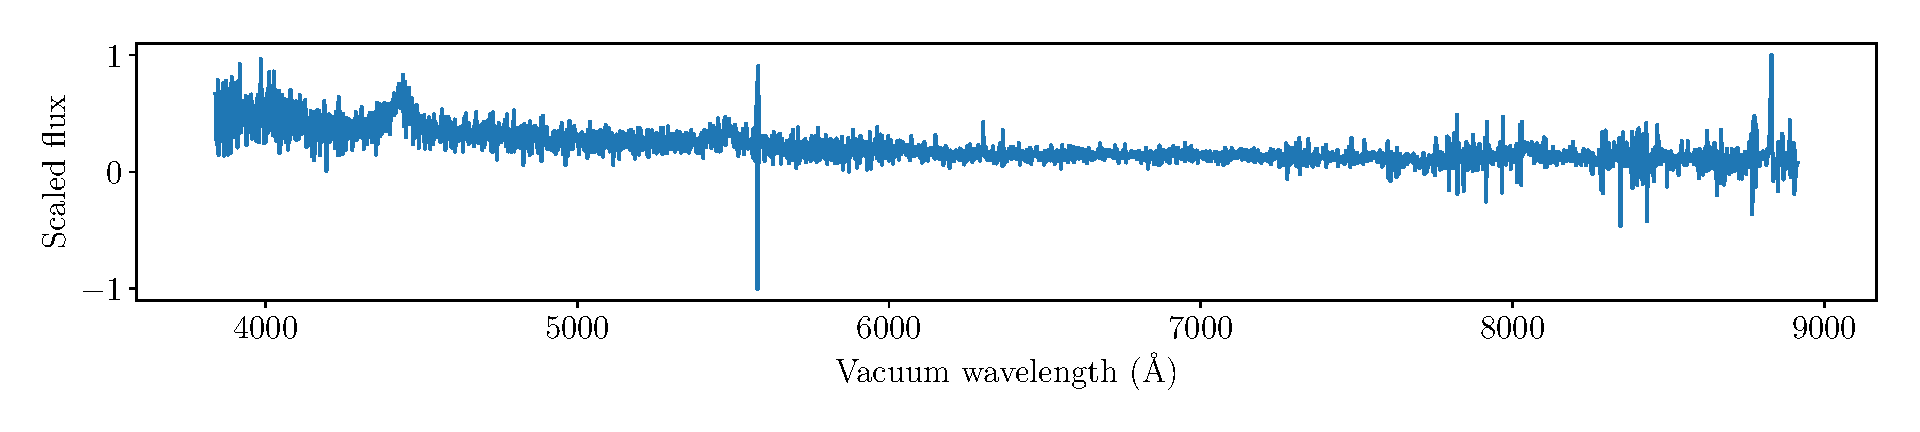
\includegraphics[width=\textwidth]{img/src_fp/spec-0406-51900-0598.pdf}
}\\
\subfloat[][\texttt{spec-0560-52296-0199}]{
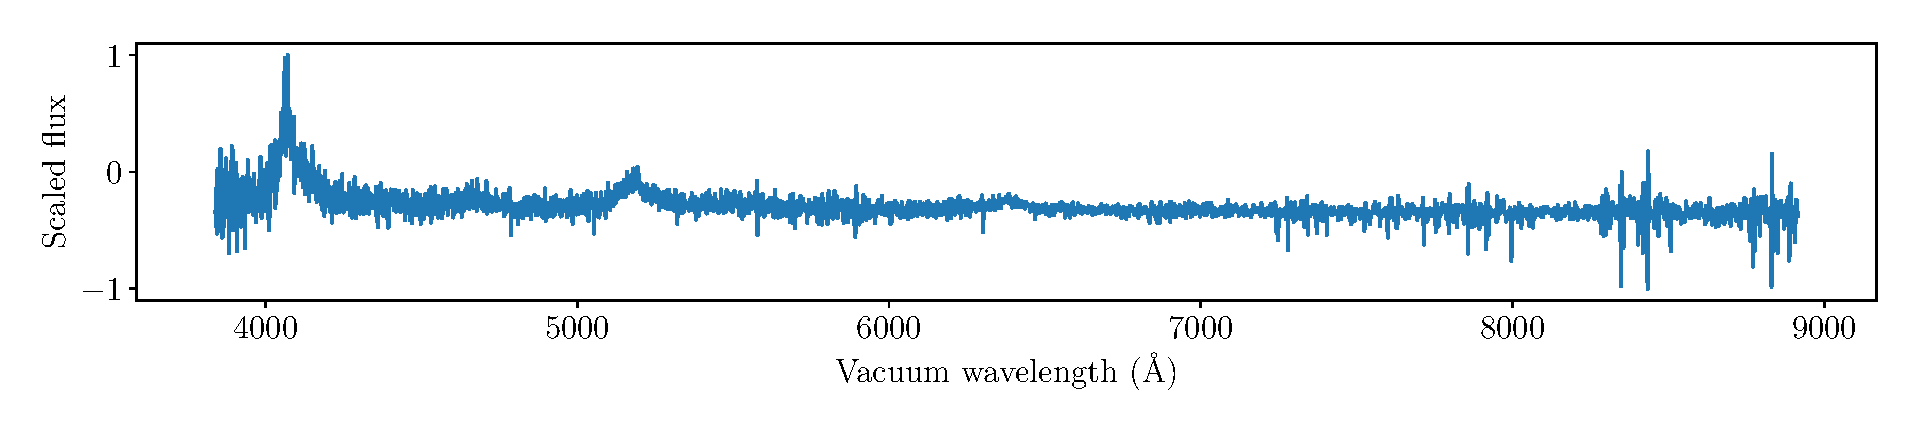
\includegraphics[width=\textwidth]{img/src_fp/spec-0560-52296-0199.pdf}
}\\
\subfloat[][\texttt{spec-0620-52081-0223}]{
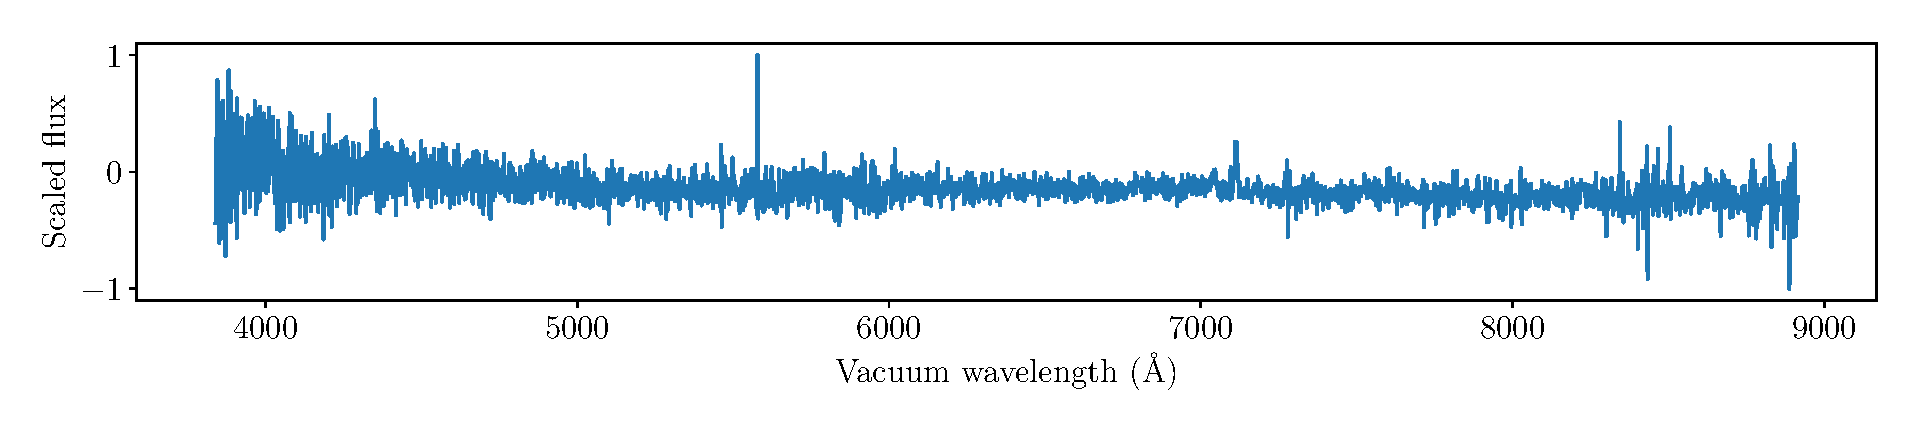
\includegraphics[width=\textwidth]{img/src_fp/spec-0620-52081-0223.pdf}
}\\
\subfloat[][\texttt{spec-0713-52178-0031}]{
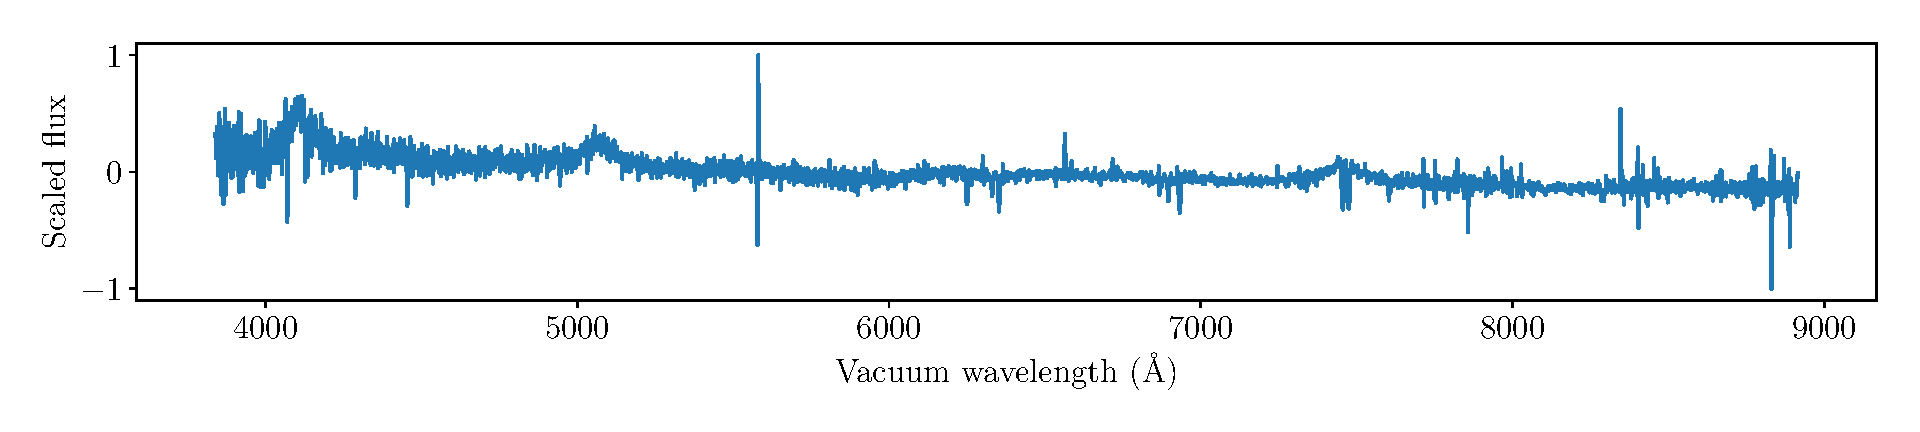
\includegraphics[width=\textwidth]{img/src_fp/spec-0713-52178-0031.pdf}
}\\
\subfloat[][\texttt{spec-0769-54530-0502}]{
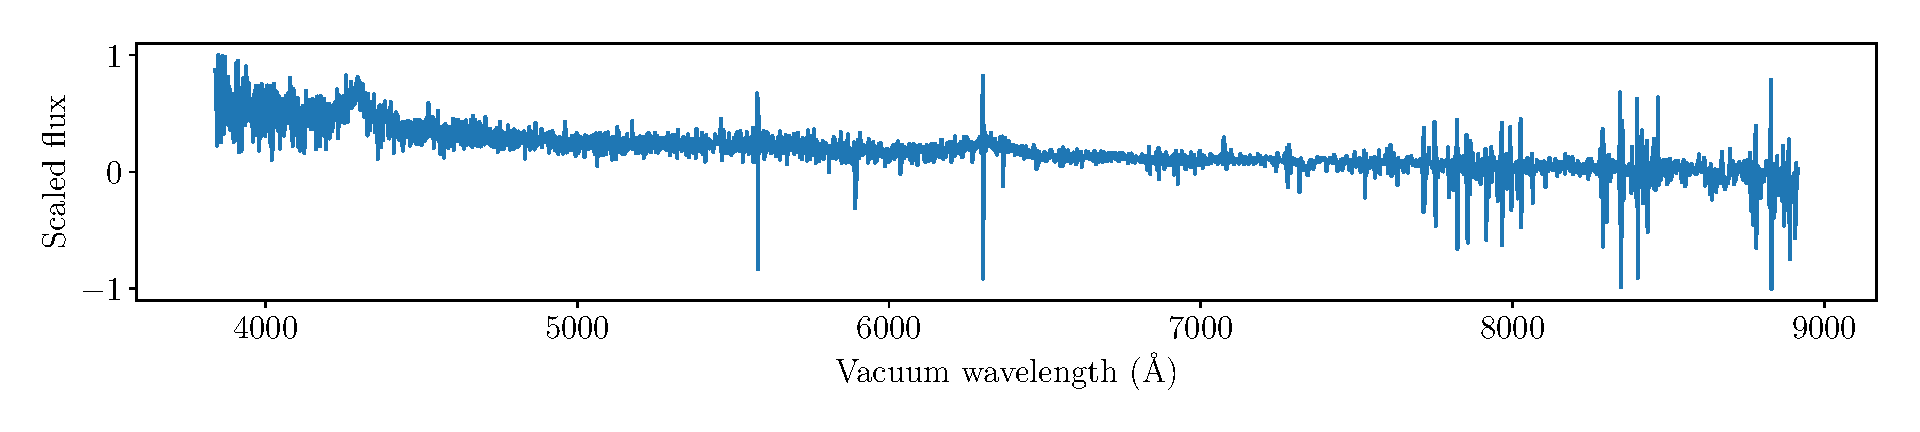
\includegraphics[width=\textwidth]{img/src_fp/spec-0769-54530-0502.pdf}
}
\caption{First sample of source false positives}
\label{src_fp}
\end{figure}

\begin{figure}
\subfloat[][\texttt{spec-56627-HD095359N274143M01\_sp09-194}]{
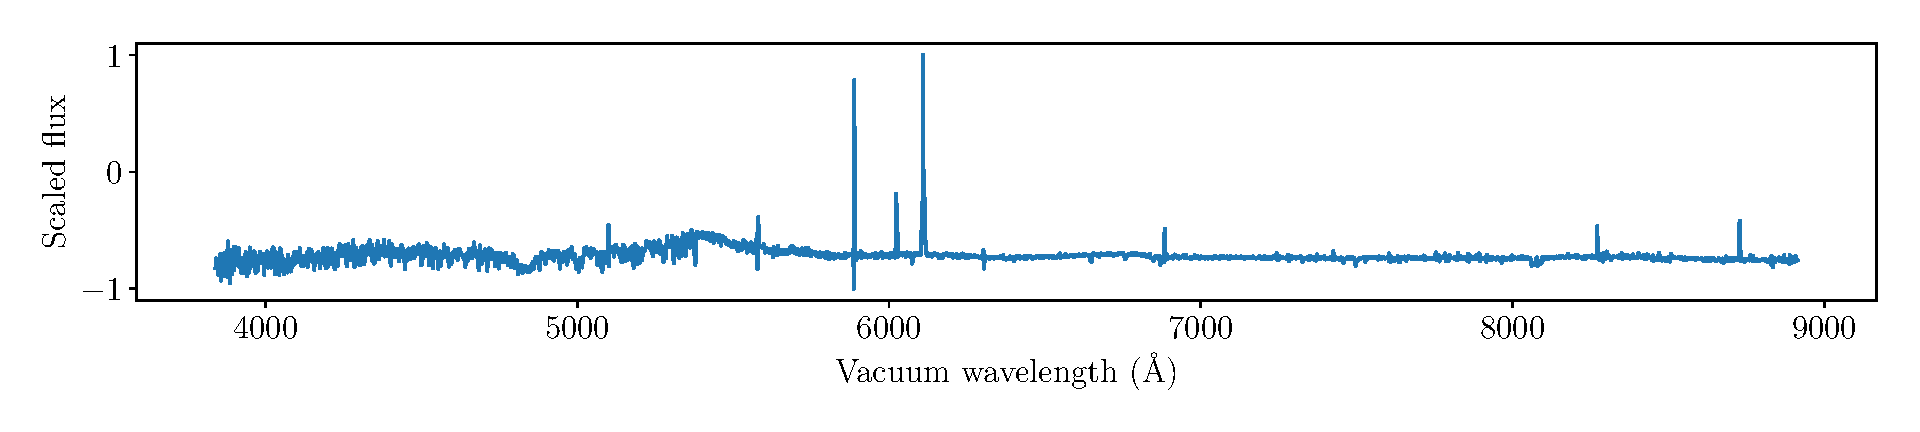
\includegraphics[width=\textwidth]{img/trg_fn/spec-56627-HD095359N274143M01_sp09-194.pdf}
}\\
\subfloat[][\texttt{spec-57163-HD163226N274234M01\_sp13-166}]{
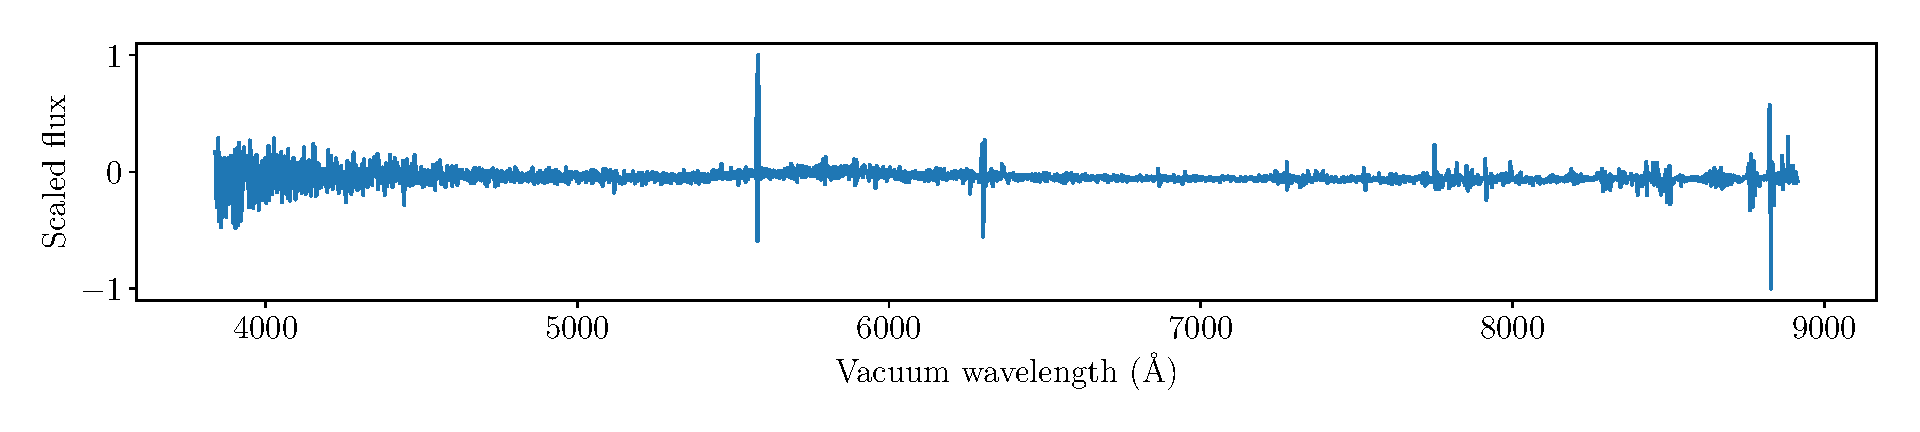
\includegraphics[width=\textwidth]{img/trg_fn/spec-57163-HD163226N274234M01_sp13-166.pdf}
}\\
\subfloat[][\texttt{spec-57284-EG234322N101953M01\_sp04-154}]{
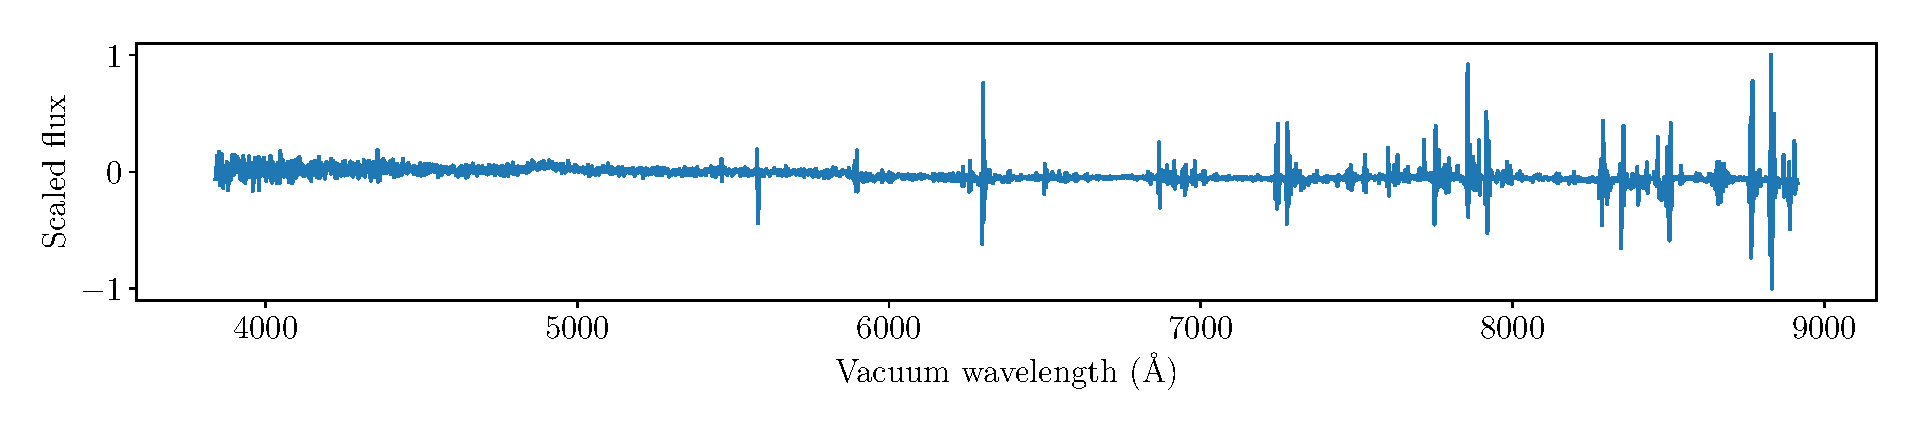
\includegraphics[width=\textwidth]{img/trg_fn/spec-57284-EG234322N101953M01_sp04-154.pdf}
}\\
\subfloat[][\texttt{spec-57367-GAC100N13M1\_sp14-011}]{
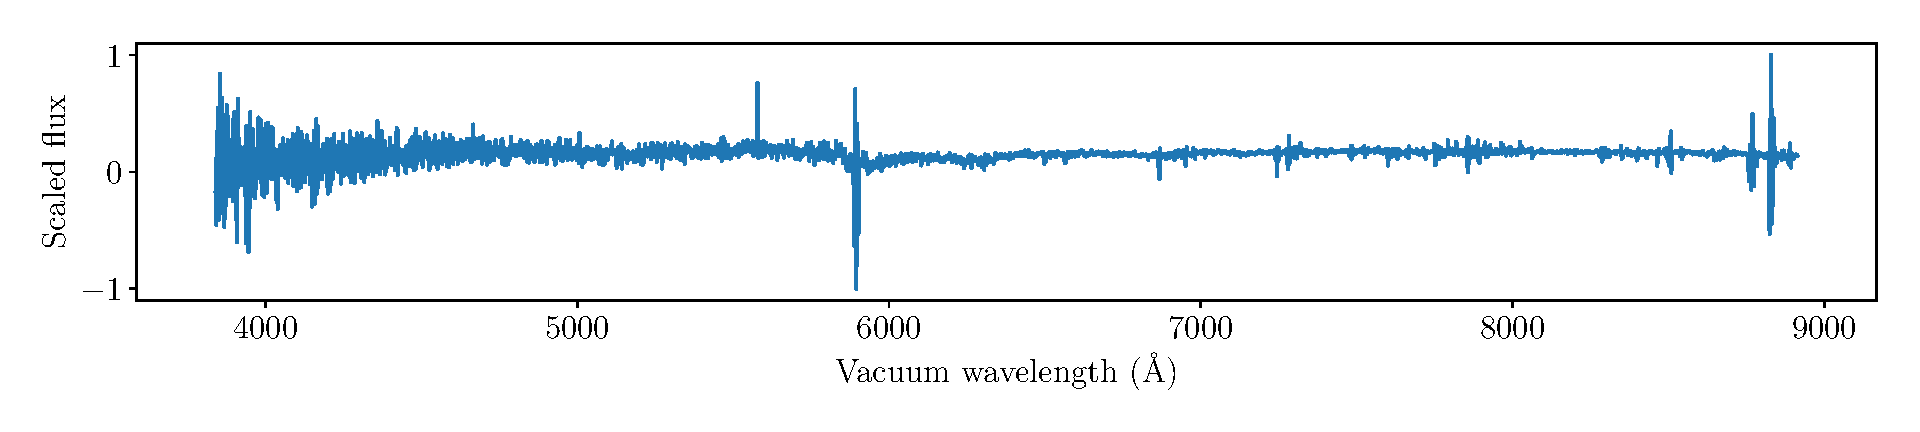
\includegraphics[width=\textwidth]{img/trg_fn/spec-57367-GAC100N13M1_sp14-011.pdf}
}\\
\subfloat[][\texttt{spec-57388-EG015238N022953M01\_sp11-103}]{
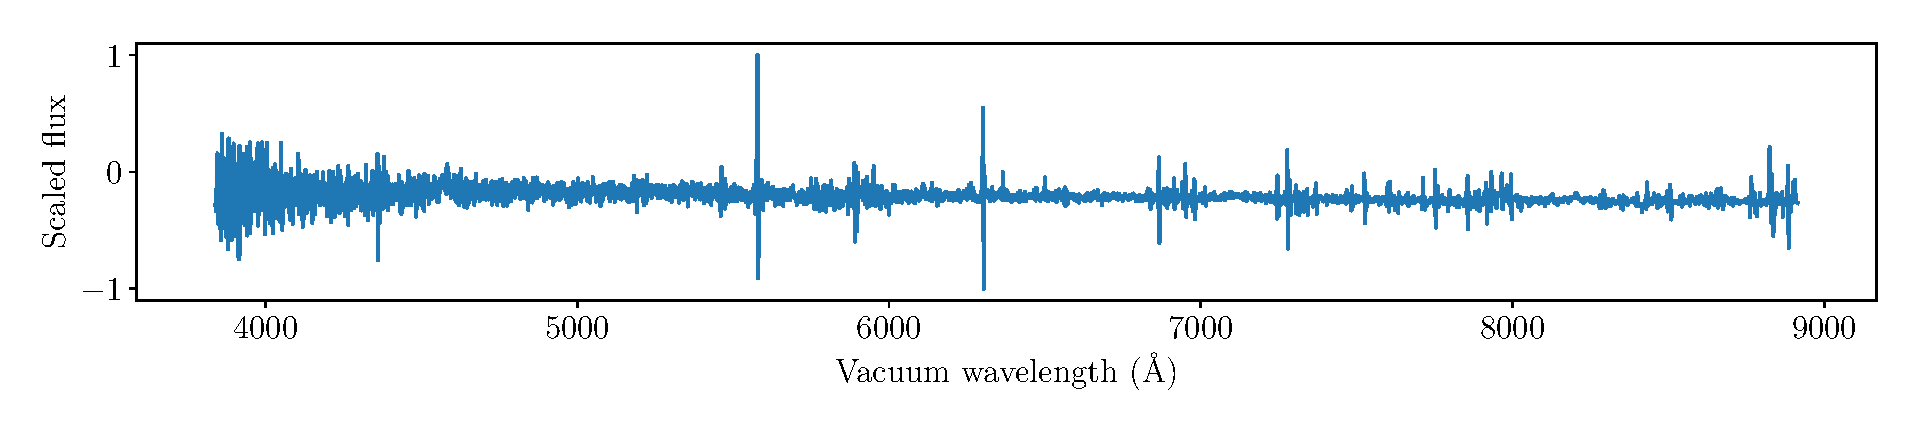
\includegraphics[width=\textwidth]{img/trg_fn/spec-57388-EG015238N022953M01_sp11-103.pdf}
}
\caption{First sample of target false negatives}
\label{trg_fn}
\end{figure}

\begin{figure}
\subfloat[][\texttt{spec-56201-EG214025S065830V02\_sp16-165}]{
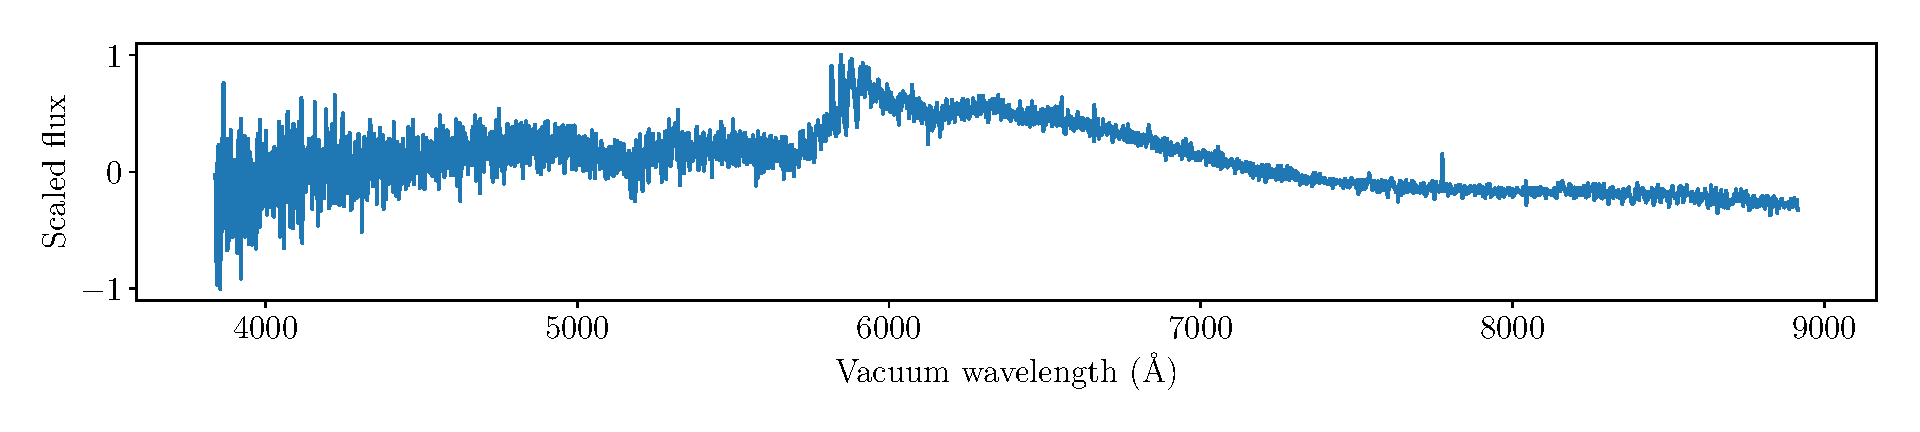
\includegraphics[width=\textwidth]{img/trg_fp/spec-56201-EG214025S065830V02_sp16-165.pdf}
}\\
\subfloat[][\texttt{spec-56225-GAC051N24B1\_sp10-104}]{
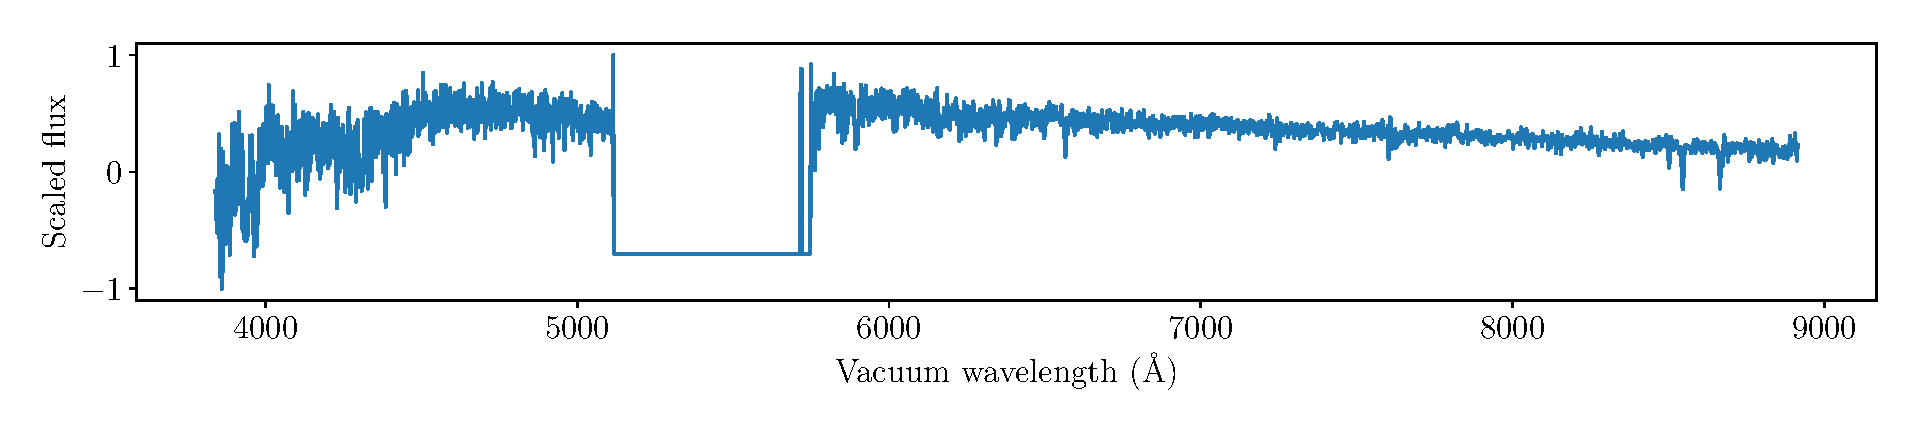
\includegraphics[width=\textwidth]{img/trg_fp/spec-56225-GAC051N24B1_sp10-104.pdf}
}\\
\subfloat[][\texttt{spec-56299-GAC096N32B1\_sp08-170}]{
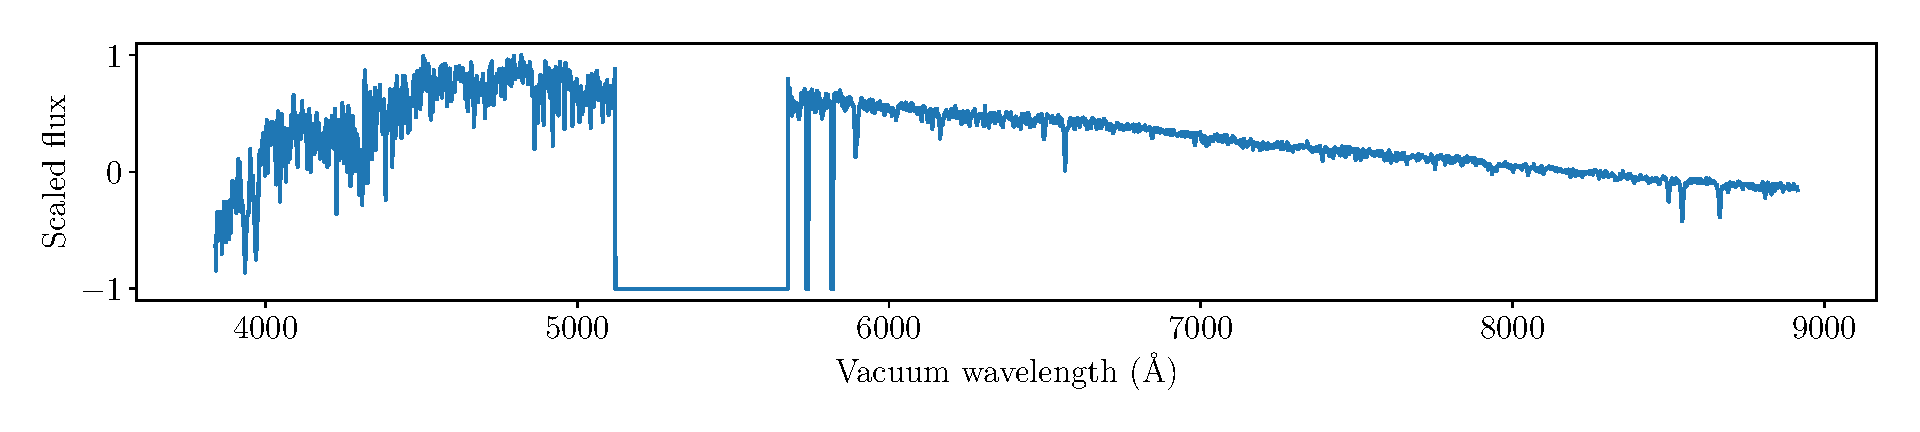
\includegraphics[width=\textwidth]{img/trg_fp/spec-56299-GAC096N32B1_sp08-170.pdf}
}\\
\subfloat[][\texttt{spec-56304-GAC094N27M1\_sp10-105}]{
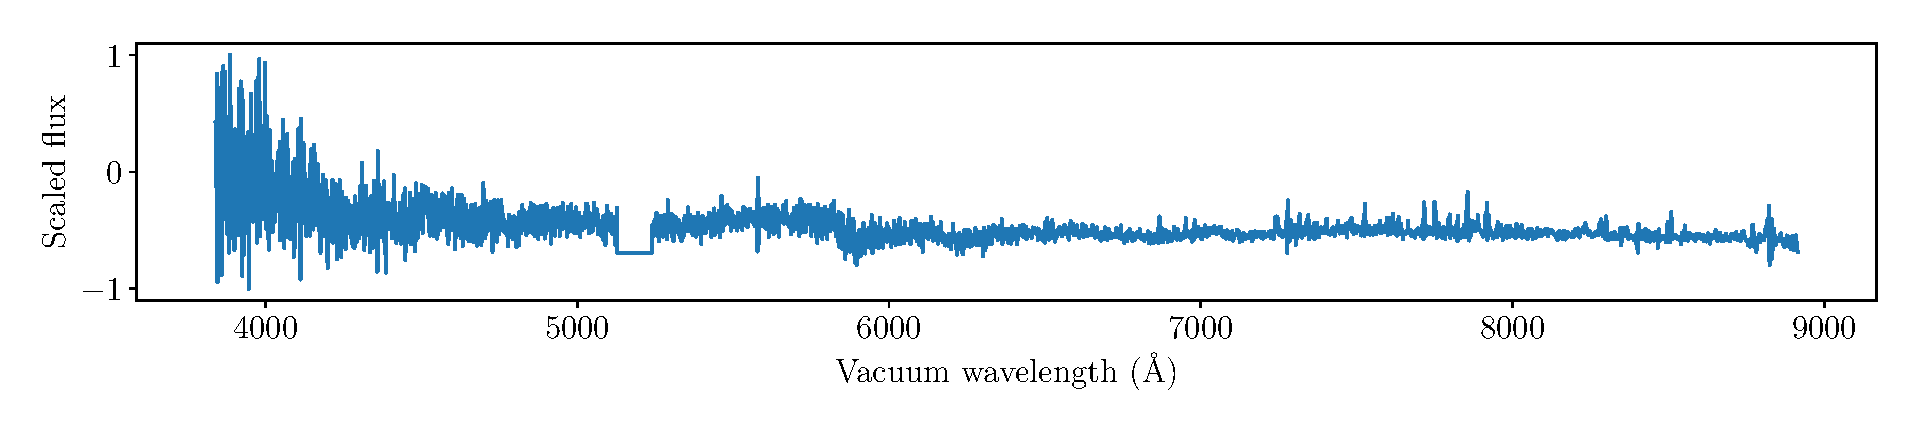
\includegraphics[width=\textwidth]{img/trg_fp/spec-56304-GAC094N27M1_sp10-105.pdf}
}\\
\subfloat[][\texttt{spec-56344-GAC088N41V3\_sp08-176}]{
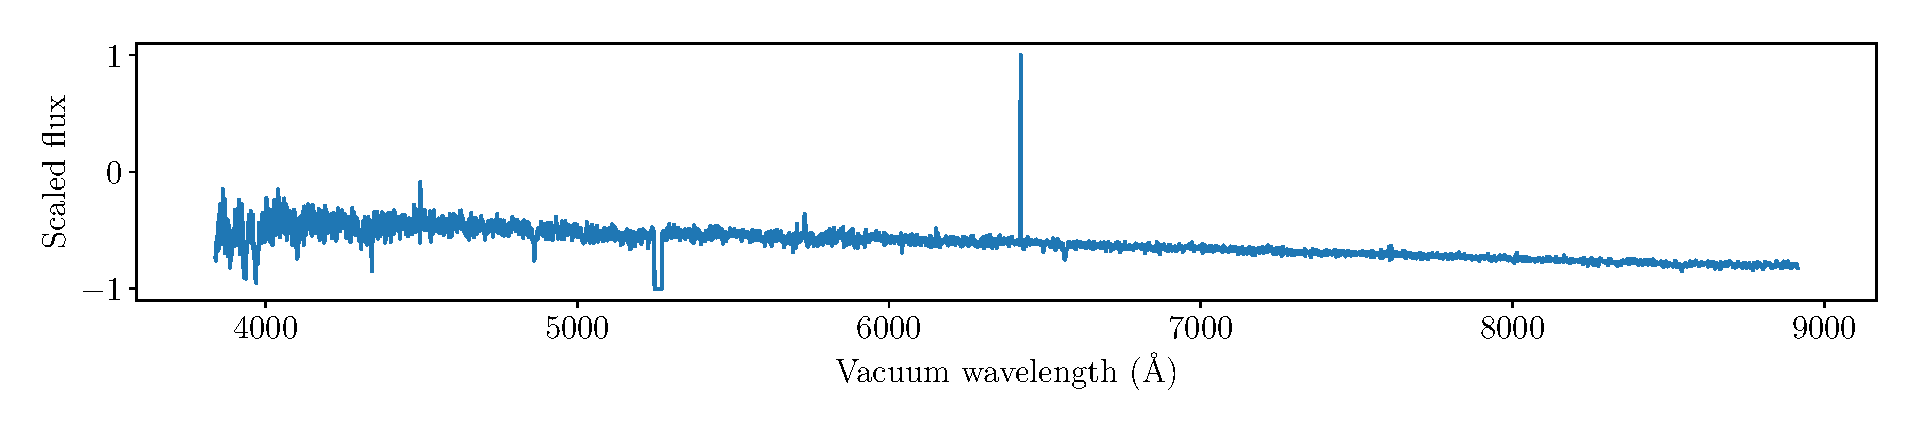
\includegraphics[width=\textwidth]{img/trg_fp/spec-56344-GAC088N41V3_sp08-176.pdf}
}
\caption{First sample of target false positives}
\label{trg_fp}
\end{figure}


\chapter{Conclusion}

\section{Discussion of Performance}

Discuss the precision performance and scalability of various solutions.

\section{Future Plans}

Suggest future improvements.

\bibliographystyle{iso690}
\bibliography{references}

\appendix

\chapter{Acronyms}

\begin{description}
	\item[AGN] Active galactic nucleus
	\item[CDD] Charge-coupled device
	\item[CORAL] Correlation Alignment
	\item[CNN] Convolutional neural network
	\item[DANN] Domain-Adversarial Neural Networks
	\item[DDC] Deep Domain Confusion
	\item[DeCAF] Deep Convolutional Activation Feature
	\item[DRCN] Deep Reconstruction-Classification Network
	\item[GPU] Graphics processing unit
	\item[LAMOST] Large Sky Area Multi-Object Fiber Spectroscopis Telescope
	\item[QSO] Quasar, Quasi-stellar object
	\item[SDSS] Sloan Digital Sky Survey
	\item[t-SNE] t-Distributed Stochastic Neighbor Embedding
	\item[UMAP] Uniform Manifold Approximation and Projection
\end{description}

\chapter{Contents of Enclosed CD}

\begin{figure}
\dirtree{%
    .1 README.md\DTcomment{the file with CD contents description}.
    .1 src\DTcomment{the directory of source codes}.
    .2 latex\DTcomment{the directory of \LaTeX{} source codes of the thesis}.
    .1 thesis.pdf\DTcomment{the thesis text in PDF format}.
}
\end{figure}

\end{document}
